% ====================================================================
% graphite_ica_ch1_Opus_v5.tex — Chapter 1 (v5 by Opus: v4 §1.1~§1.17 의 수식-구동 재표현)
%   흑연 음극 dQ/dV(ICA) 이론 — 반응속도론(Eyring) 척추 구성.
%   v5 = v4 의 산문(글귀)을 최소화하고 논리 전개의 절대 다수를 수식 사슬이 운반하도록
%        재표현한 버전("수식만 따라가도 이해"). 모든 식·figure 는 v4 verbatim,
%        식 사이 산문은 연결 한 줄로, 산문-only 유도단계는 명시 중간식으로 승격.
%   범위 = §1.1~§1.17 (v4 의 §1.18 [확장] 적층 준안정은 제외).
%   build: xelatex 2-pass (kotex — 한글 포함 verbatim 은 XeLaTeX 전제)
% ====================================================================
\documentclass[11pt,a4paper]{article}
\usepackage[margin=22mm]{geometry}
\usepackage{kotex}
\setmonofont{D2Coding}[Scale=MatchLowercase]
\usepackage{amsmath,amssymb,mathtools,bm}
\usepackage{booktabs,longtable,array}
\usepackage{enumitem}
\usepackage{amsthm}
\usepackage{hyperref}
\usepackage{fancyhdr}
\usepackage{lastpage}
\usepackage{setspace}
\usepackage{tikz}
\usetikzlibrary{positioning}
\setstretch{1.12}
\setlength{\parskip}{0.45em}\setlength{\parindent}{0pt}\setlength{\headheight}{14pt}
\setlength{\emergencystretch}{2em}% 긴 인라인식이 줄끝에 걸린 정당 줄을 마지막 패스에서 흡수(overfull 0; 내용 불변)
\hypersetup{colorlinks=true, linkcolor=blue, urlcolor=blue, citecolor=blue,
  pdftitle={흑연 음극 dQ/dV 이론: 수식-구동 — Chapter 1 (v5)}}
\pagestyle{fancy}\fancyhf{}
\lhead{흑연 음극 $dQ/dV$ 이론 — Ch.1 (v5, 수식-구동)}\rhead{\thepage/\pageref{LastPage}}
\renewcommand{\headrulewidth}{0.4pt}

\newtheorem*{keybox}{핵심}
\newtheorem*{stagebox}{흑연 staging 배경}
\newtheorem*{boundbox}{유효 범위}
\newtheorem*{verifybox}{검산}

\newcommand{\dd}{\mathrm{d}}
\newcommand{\eff}{\mathrm{eff}}
\newcommand{\eq}{\mathrm{eq}}
\newcommand{\app}{\mathrm{app}}
\newcommand{\drive}{\mathrm{drive}}
\newcommand{\cell}{\mathrm{cell}}
\newcommand{\bg}{\mathrm{bg}}
\newcommand{\ext}{\mathrm{ext}}
\newcommand{\OCV}{\mathrm{OCV}}
\newcommand{\sstat}{\mathrm{ss}}
\newcommand{\peak}{\mathrm{peak}}
\newcommand{\dis}{\mathrm{dis}}
\newcommand{\chg}{\mathrm{chg}}
\newcommand{\hys}{\mathrm{hys}}
\newcommand{\pol}{\mathrm{pol}}
\newcommand{\obs}{\mathrm{obs}}

\renewcommand{\theequation}{1.\arabic{equation}}
\renewcommand{\thesection}{1.\arabic{section}}
\title{\textbf{\LARGE Chapter 1}\\[0.35em]\Large 흑연 음극 $dQ/dV$ 이론: 하나의 속도식에서 피팅까지 — 수식-구동판}
\author{}
\date{}

% TOC: widen number boxes (two-digit section numbers overflow article's 1.5em default)
\makeatletter
\renewcommand*\l@section[2]{%
  \ifnum \c@tocdepth >\z@
    \addpenalty\@secpenalty
    \addvspace{1.0em \@plus\p@}%
    \setlength\@tempdima{2.3em}%
    \begingroup
      \parindent \z@ \rightskip \@pnumwidth
      \parfillskip -\@pnumwidth
      \leavevmode \bfseries
      \advance\leftskip\@tempdima
      \hskip -\leftskip
      #1\nobreak\hfil
      \nobreak\hb@xt@\@pnumwidth{\hss #2\kern-\p@\kern\p@}\par
    \endgroup
  \fi}
\renewcommand*\l@subsection{\@dottedtocline{2}{2.3em}{3.2em}}
\makeatother

\begin{document}
\maketitle

% ====================================================================
\section*{서론}
\addcontentsline{toc}{section}{서론}
% ====================================================================
리튬이온전지 흑연 음극의 \textbf{incremental capacity analysis}(ICA)는 충방전 곡선 $Q(V)$ 의 미분
$\dd Q/\dd V$ 를 본다 \cite{bloom2005,dubarry2012}. 흑연은 staging 상전이(stage
$4\!\to\!3\!\to\!2\mathrm L\!\to\!2\!\to\!1$; $2\mathrm L$ 은 stage-2 의 면내 질서가 풀린 단계)를 거치며
\cite{dahn1991,ohzuku1993,funabiki1999}, 각 전이 전위에서 두 상이 공존하면 전위가 거의 평탄($\dd V_n/\dd q\to0$)이라
좁은 $\dd V$ 에 큰 $\dd Q$ 가 몰려 $\dd Q/\dd V$ 가 치솟는다 — ``전위 평탄 구간 $=$ ICA peak''가 본 문건의 대상이다.

\textbf{관측.}
\begin{quote}\itshape
$\dd Q/\dd V$ 상전이 peak 의 \textbf{위치$\cdot$너비$\cdot$높이}는 \textbf{(a) 온도, (b) 극판 전위, (c) C-rate(전류)}
세 가지에 따라 변한다. 저온$\cdot$고율일수록 peak 의 꼬리가 길어져 다음 peak 와 겹치고, 같은 전이가 충전과 방전에서 서로 다른
전위에 peak 를 남기며(충방전 히스테리시스), 이 갈림에는 전류를 $0$ 으로 줄여도 사라지지 않는 성분이 있다.
\end{quote}

\textbf{하나의 속도식.} 세 인자는 활성화 장벽을 넘는 반응의 속도식
\begin{equation*}
k\;\simeq\;k_0\,\exp\!\Big[-\frac{\Delta G_a}{RT}\Big]
\end{equation*}
의 세 갈래다(\S\ref{sec:rate} 식~\eqref{eq:eyring} 로 정식화). 온도는 지수의 분모, 전위는 장벽 $\Delta G_a$ 자체,
C-rate 는 $k$ 와 요구 전환 속도의 경쟁으로 들어오고, 평형조차 정$\cdot$역 속도가 같아지는 정지점으로 이 식에서 회수된다
(\S\ref{sec:fwdrev}). 주 전개는 방전(탈리튬화) $\dd Q/\dd V$ 이며(\S\ref{sec:rate}--\S\ref{sec:overlap}), 충방전 히스테리시스는
그 위의 확장(\S\ref{sec:hys} 이하)이다. 도착점은 한 줄 피팅식과 알고리즘(\S\ref{sec:master}$\cdot$\S\ref{sec:code})과
반증 조건(\S\ref{sec:falsify})이다.

흑연 staging 의 갤러리 채움(리튬화 방향 $4\to3\to2\mathrm L\to2\to1$, 방전은 역순 $\theta_j:1\to0$)을 그림~\ref{fig:staging}
에 둔다 — 각 stage 전이가 $\dd Q/\dd V$ 에 peak 하나를 남기고, 중심 간격이 전이폭 이하인 인접 전이는 융합해 관측 유효 전이 수가
$N_p\approx3$--$4$ 가 된다.

\begin{figure}[t]
\centering
\begin{tikzpicture}[x=0.95cm,y=0.95cm]
\fill[black!70] (0.0,0.315) rectangle (1.6,0.525);
\fill[black!70] (0.0,1.435) rectangle (1.6,1.645);
\fill[black!70] (0.0,2.555) rectangle (1.6,2.765);
\draw[semithick] (0.0,0.00) -- (1.6,0.00);
\draw[semithick] (0.0,0.28) -- (1.6,0.28);
\draw[semithick] (0.0,0.56) -- (1.6,0.56);
\draw[semithick] (0.0,0.84) -- (1.6,0.84);
\draw[semithick] (0.0,1.12) -- (1.6,1.12);
\draw[semithick] (0.0,1.40) -- (1.6,1.40);
\draw[semithick] (0.0,1.68) -- (1.6,1.68);
\draw[semithick] (0.0,1.96) -- (1.6,1.96);
\draw[semithick] (0.0,2.24) -- (1.6,2.24);
\draw[semithick] (0.0,2.52) -- (1.6,2.52);
\draw[semithick] (0.0,2.80) -- (1.6,2.80);
\draw[semithick] (0.0,3.08) -- (1.6,3.08);
\draw[semithick] (0.0,3.36) -- (1.6,3.36);
\node[below,align=center] at (0.8,-0.08) {\scriptsize stage 4};
\fill[black!70] (2.2,0.315) rectangle (3.8,0.525);
\fill[black!70] (2.2,1.155) rectangle (3.8,1.365);
\fill[black!70] (2.2,1.995) rectangle (3.8,2.205);
\fill[black!70] (2.2,2.835) rectangle (3.8,3.045);
\draw[semithick] (2.2,0.00) -- (3.8,0.00);
\draw[semithick] (2.2,0.28) -- (3.8,0.28);
\draw[semithick] (2.2,0.56) -- (3.8,0.56);
\draw[semithick] (2.2,0.84) -- (3.8,0.84);
\draw[semithick] (2.2,1.12) -- (3.8,1.12);
\draw[semithick] (2.2,1.40) -- (3.8,1.40);
\draw[semithick] (2.2,1.68) -- (3.8,1.68);
\draw[semithick] (2.2,1.96) -- (3.8,1.96);
\draw[semithick] (2.2,2.24) -- (3.8,2.24);
\draw[semithick] (2.2,2.52) -- (3.8,2.52);
\draw[semithick] (2.2,2.80) -- (3.8,2.80);
\draw[semithick] (2.2,3.08) -- (3.8,3.08);
\draw[semithick] (2.2,3.36) -- (3.8,3.36);
\node[below,align=center] at (3.0,-0.08) {\scriptsize stage 3};
\fill[black!25] (4.4,0.315) rectangle (6.0,0.525);
\fill[black!25] (4.4,0.875) rectangle (6.0,1.085);
\fill[black!25] (4.4,1.435) rectangle (6.0,1.645);
\fill[black!25] (4.4,1.995) rectangle (6.0,2.205);
\fill[black!25] (4.4,2.555) rectangle (6.0,2.765);
\fill[black!25] (4.4,3.115) rectangle (6.0,3.325);
\draw[semithick] (4.4,0.00) -- (6.0,0.00);
\draw[semithick] (4.4,0.28) -- (6.0,0.28);
\draw[semithick] (4.4,0.56) -- (6.0,0.56);
\draw[semithick] (4.4,0.84) -- (6.0,0.84);
\draw[semithick] (4.4,1.12) -- (6.0,1.12);
\draw[semithick] (4.4,1.40) -- (6.0,1.40);
\draw[semithick] (4.4,1.68) -- (6.0,1.68);
\draw[semithick] (4.4,1.96) -- (6.0,1.96);
\draw[semithick] (4.4,2.24) -- (6.0,2.24);
\draw[semithick] (4.4,2.52) -- (6.0,2.52);
\draw[semithick] (4.4,2.80) -- (6.0,2.80);
\draw[semithick] (4.4,3.08) -- (6.0,3.08);
\draw[semithick] (4.4,3.36) -- (6.0,3.36);
\node[below,align=center] at (5.2,-0.08) {\scriptsize stage $2\mathrm L$};
\fill[black!70] (6.6,0.315) rectangle (8.2,0.525);
\fill[black!70] (6.6,0.875) rectangle (8.2,1.085);
\fill[black!70] (6.6,1.435) rectangle (8.2,1.645);
\fill[black!70] (6.6,1.995) rectangle (8.2,2.205);
\fill[black!70] (6.6,2.555) rectangle (8.2,2.765);
\fill[black!70] (6.6,3.115) rectangle (8.2,3.325);
\draw[semithick] (6.6,0.00) -- (8.2,0.00);
\draw[semithick] (6.6,0.28) -- (8.2,0.28);
\draw[semithick] (6.6,0.56) -- (8.2,0.56);
\draw[semithick] (6.6,0.84) -- (8.2,0.84);
\draw[semithick] (6.6,1.12) -- (8.2,1.12);
\draw[semithick] (6.6,1.40) -- (8.2,1.40);
\draw[semithick] (6.6,1.68) -- (8.2,1.68);
\draw[semithick] (6.6,1.96) -- (8.2,1.96);
\draw[semithick] (6.6,2.24) -- (8.2,2.24);
\draw[semithick] (6.6,2.52) -- (8.2,2.52);
\draw[semithick] (6.6,2.80) -- (8.2,2.80);
\draw[semithick] (6.6,3.08) -- (8.2,3.08);
\draw[semithick] (6.6,3.36) -- (8.2,3.36);
\node[below,align=center] at (7.4,-0.08) {\scriptsize stage 2 ($\mathrm{LiC_{12}}$)};
\fill[black!70] (8.8,0.035) rectangle (10.4,0.245);
\fill[black!70] (8.8,0.315) rectangle (10.4,0.525);
\fill[black!70] (8.8,0.595) rectangle (10.4,0.805);
\fill[black!70] (8.8,0.875) rectangle (10.4,1.085);
\fill[black!70] (8.8,1.155) rectangle (10.4,1.365);
\fill[black!70] (8.8,1.435) rectangle (10.4,1.645);
\fill[black!70] (8.8,1.715) rectangle (10.4,1.925);
\fill[black!70] (8.8,1.995) rectangle (10.4,2.205);
\fill[black!70] (8.8,2.275) rectangle (10.4,2.485);
\fill[black!70] (8.8,2.555) rectangle (10.4,2.765);
\fill[black!70] (8.8,2.835) rectangle (10.4,3.045);
\fill[black!70] (8.8,3.115) rectangle (10.4,3.325);
\draw[semithick] (8.8,0.00) -- (10.4,0.00);
\draw[semithick] (8.8,0.28) -- (10.4,0.28);
\draw[semithick] (8.8,0.56) -- (10.4,0.56);
\draw[semithick] (8.8,0.84) -- (10.4,0.84);
\draw[semithick] (8.8,1.12) -- (10.4,1.12);
\draw[semithick] (8.8,1.40) -- (10.4,1.40);
\draw[semithick] (8.8,1.68) -- (10.4,1.68);
\draw[semithick] (8.8,1.96) -- (10.4,1.96);
\draw[semithick] (8.8,2.24) -- (10.4,2.24);
\draw[semithick] (8.8,2.52) -- (10.4,2.52);
\draw[semithick] (8.8,2.80) -- (10.4,2.80);
\draw[semithick] (8.8,3.08) -- (10.4,3.08);
\draw[semithick] (8.8,3.36) -- (10.4,3.36);
\node[below,align=center] at (9.6,-0.08) {\scriptsize stage 1 ($\mathrm{LiC_6}$)};
\draw[->,thick] (0,3.81) -- (10.4,3.81) node[pos=0.5,above] {\footnotesize 리튬화(충전) — 채움 순서 $4\to3\to2\mathrm L\to2\to1$, stage 번호 $n$ $=$ 채운 층 사이의 빈 갤러리 $n-1$ 개};
\draw[<-,thick] (0,-0.75) -- (10.4,-0.75) node[pos=0.5,below] {\footnotesize 방전(탈리튬화) — 본 문건의 주 전개 방향(역순), $\theta_j$ 가 $1\to0$ 으로 줄어든다};
\end{tikzpicture}
\caption{흑연 staging 의 갤러리 채움 도식. 수평선이 그래핀 층, 음영 띠가 리튬이 든 층간
갤러리다. 채울수록 stage 번호가 줄어 stage 1($\mathrm{LiC_6}$, 완전 채움)에 닿고, 각 stage 전이가
$\dd Q/\dd V$ 에 peak 하나를 남긴다. stage $2\mathrm L$ 은 stage 2 와 같은 주기이되 갤러리 안이
희박하고 면내 질서가 풀린(liquid-like) 단계라 옅게 표시했다. 개념도이며 — 실제 채움은 갤러리 전체가
아니라 국소 도메인 단위로 진행되고 층의 굽힘을 동반한다(Daumas--H\'erold 그림, \S\ref{sec:thermo}).}
\label{fig:staging}
\end{figure}

\tableofcontents
\newpage

% ====================================================================
\section{기호와 규약}\label{sec:notation}
% ====================================================================
표는 식~\eqref{eq:eyring}$\cdot$\eqref{eq:mu} 류 보편식부터 관측축$\cdot$꼬리까지 본 문건 전개 순서대로 배열된 사전이다.

\textbf{전이 인덱스.} $j=1,\dots,N_p$($N_p\approx3\text{--}4$). 전이 $j$ 마다 점유율 $\theta_j$, 진행률 $\xi_j\equiv1-\theta_j$(방전 시 $\theta_j:1\to0$, $\xi_j:0\to1$). 박스 결과식은 항상 $j$ 첨자(보편식 식~\eqref{eq:eyring}$\cdot$\eqref{eq:mu} 류만 예외).

\textbf{부호 규약.} 모든 전위는 흑연 음극 반쪽전지 전위(vs Li/Li$^+$; full-cell 측정은 \S\ref{sec:master} 환산 선행). 진행 방향 부호 $s\in\{+1,-1\}$, 방전 기준 $s=+1$ 고정(평형 곡선은 진행 방향에 불변인 상태함수이므로 정의 안에 $+1$ 로 고정). 전류 부호 $s_I$(방전 $+1$)는 분극 부호 약속 $V_\app=V_n+s_I|I|R_n$(식~\eqref{eq:vapp})에 들어간다 — 방전$=$산화 방향이라 분극이 측정 전위를 내부 전위 위로 올린다(\S\ref{sec:charge}). 충방전 양방향 방향 부호 $\sigma_d=\pm1$ 은 \S\ref{sec:master} 에서 도입하며, 그 작용처는 분극 부호$\cdot$분기 중심 선택$\cdot$꼬리 지지/감쇠 방향 셋이다($s_I$ 는 방전 본론 한정 표기 — 양방향 통합식부터 $\sigma_d$ 가 흡수).

\begin{longtable}{p{0.15\textwidth} p{0.13\textwidth} p{0.64\textwidth}}
\toprule 기호 & 단위 & 의미 \\ \midrule \endhead
\multicolumn{3}{l}{\emph{— 속도식과 장벽(\S\ref{sec:rate}$\cdot$\S\ref{sec:fwdrev}$\cdot$\S\ref{sec:potbranch}) —}}\\
$k_j,\ k_0$ & 1/s & 전이 $j$ 의 완화 속도상수($=r_j^++r_j^-$; 보편식 무첨자 $k$ 는 한 방향 사건 속도), Eyring prefactor $k_0=k_BT/h$ \\
$\Delta G_{a,j}$ & J/mol & 활성화 자유에너지 $=\Delta H_{a,j}-T\Delta S_{a,j}$ \\
$\Delta H_{a,j},\Delta S_{a,j}$ & {\footnotesize J/mol;\,J/(mol\,K)} & 활성화 엔탈피$\cdot$엔트로피(\emph{속도}에 들어가는 양 — 반응 엔트로피 $\Delta S_j$ 와 다르다) \\
$r_j^\pm$ & 1/s & 전이 $j$ 의 정(탈리튬화)/역(재리튬화) 방향 속도 \\
$\chi$ & --- & 전달 계수 $0\le\chi\le1$(표준 표기 $\alpha$) \\
$\mathcal A_j$ & J/mol & 구동력(affinity) $=sF(V_\drive-U_j)$; 일반형에 $-\Omega_j(1-2\xi_j)$ 합류(\S\ref{sec:regsol}) \\
$\Delta G_{\eff,j}$ & J/mol & 유효 활성화 자유에너지 $=\Delta G_{a,j}-\chi\mathcal A_j$ \\
$k_j^{\eff},k_{j,\lim}$ & 1/s & 직렬 율속 합성 $1/k_j^{\eff}=1/k_j+1/k_{j,\lim}$ 의 유효 속도$\cdot$공율속 \\
$\lambda$ & J/mol & Marcus 재구성 에너지(선형 근사 한계 척도) \\
\multicolumn{3}{l}{\emph{— 열역학(\S\ref{sec:thermo}$\cdot$\S\ref{sec:regsol}) —}}\\
$G,\ \mu$ & J;\,J/mol & Gibbs 자유에너지, 화학퍼텐셜 $\mu=\partial G/\partial n$ \\
$\mu^0,\ \tilde\mu$ & J/mol & 기준 화학퍼텐셜, 전기화학 퍼텐셜 $=\mu+zF\phi$ \\
$\theta_j$ & --- & 전이 $j$ 의 Li 점유율(방전 시 $1\to0$) \\
$\xi_j,\ \xi_{\eq,j},\ \xi_{\sstat,j}$ & --- & 진행률 $=1-\theta_j$, 평형값, 정지점값(\S\ref{sec:fwdrev}; 기본형 $\xi_{\sstat}=\xi_{\eq}$) \\
$\Omega_j$ & J/mol & 정규용액 상호작용 에너지($>2RT$ 면 상분리$\cdot$히스테리시스) \\
$U_j(T)$ & V & 전이 $j$ 의 평형 중심 전위 \\
$\Delta S_j$ & J/(mol\,K) & 삽입 반응 엔트로피($\partial U_j/\partial T=\Delta S_j/(sF)$) \\
$w_j$ & V & 전이 폭 척도(이상 극한 $RT/F$, \S\ref{sec:fwdrev}; 운용 \S\ref{sec:eqpeak}) \\
$T_{c,j},\ \xi_{s,j}^\pm,\ \xi_{b,j}^\pm$ & {\footnotesize K;\,---;\,---} & 임계 온도 $=\Omega_j/2R$; spinodal$\cdot$binodal 진행률(\S\ref{sec:regsol}) \\
\multicolumn{3}{l}{\emph{— 관측축(\S\ref{sec:charge}) —}}\\
$V_n$ & V & \emph{내부} 음극 전위 — 전하 보존식의 해 \\
$V_\app$ & V & 측정 전위 $=V_n+s_I|I|R_n$ \\
$V_\drive$ & V & 속도 구동 전위(기본형 $V_\drive=V_n$) \\
$Q_j,\ Q_\cell$ & C & 전이 $j$ 의 용량, 셀 총 방전 용량 \\
$q$ & --- & 무차원 용량 좌표 $=\int|I|\,\dd t/Q_\cell$ \\
$Q_\bg,\ C_\bg$ & C;\,C/V & 배경 누적 용량, 미분용량 $\partial Q_\bg/\partial V_n$ \\
$R_n$ & $\Omega$ & 음극 유효 분극 저항(lumped; 단위 규약 \S\ref{sec:master}) \\
\multicolumn{3}{l}{\emph{— 지연과 꼬리(\S\ref{sec:lag}$\cdot$\S\ref{sec:tempbranch}) —}}\\
$r_j$ & --- & 지연 $=\xi_{\eq,j}-\xi_j$(위첨자 없음 — 속도 $r_j^\pm$ 와 구별) \\
$L_{q,j},\ L_{V,j}$ & ---;\,V & 용량축$\cdot$전압축 꼬리 특성 길이($L_{V,j}=|\dd V_n/\dd q|_{q_a}L_{q,j}$) \\
$q_a,\ V_{a,j},\ r_{a,j}$ & ---;\,V;\,--- & 꼬리 시작 좌표$\cdot$전위$\cdot$잔류 지연 \\
$\rho_G(G),\ \sigma_G$ & mol/J;\,J/mol & 활성화 장벽의 용량-분율 밀도($\int\rho_G\dd G=1$)와 표준편차 \\
\multicolumn{3}{l}{\emph{— 충방전 확장(\S\ref{sec:hys} 이하) —}}\\
$\gamma_j$ & --- & 분기 축소 인자(다입자$\cdot$핵생성) $0\le\gamma_j\le1$ \\
$\Delta U_j^\hys$ & V & 충방전 분기 gap 의 spinodal 상한(식~\eqref{eq:hysdU}) \\
$U_j^{\dis},U_j^{\chg}$ & V & 방전$\cdot$충전 분기 중심 $=U_j\pm\tfrac12\gamma_j\Delta U_j^\hys$ \\
$\sigma_d$ & --- & 방향 부호(방전 $+1$/충전 $-1$) \\
$R,F,k_B,h,N_A$ & {\footnotesize J/(mol\,K), C/mol, J/K, J\,s, 1/mol} & 기체상수, Faraday, Boltzmann, Planck, Avogadro($R=k_BN_A$) \\
\bottomrule
\end{longtable}

% ====================================================================
\section{근본식 — 활성화 장벽과 반응 속도}\label{sec:rate}
% ====================================================================
관측은 유한 전류$\cdot$유한 시간에서 이루어지므로 관측을 지배하는 것은 속도다 — 본 문건은 속도식에서 출발한다.

\subsection{장벽 그림 — 왜 속도는 지수인가}
온도 $T$ 의 계에서 한 자유도가 몰 단위 장벽 $\Delta G_a=N_AE^*$ 이상을 우연히 갖출 확률은 Boltzmann 분포를 따른다:
\begin{equation}
P(E\ge E^*)\;\propto\;e^{-E^*/k_BT}
\;=\;e^{-\Delta G_a/RT}\qquad(R=k_BN_A).
\label{eq:boltz}
\end{equation}
속도 $=$ 시도 빈도 $\times$ 넘을 확률이고, 전이상태 이론의 보편 시도 빈도 $k_0=k_BT/h$ 를 식~\eqref{eq:boltz} 에 곱하면 \cite{eyring1935} 근본식이 된다:
\begin{equation}
\boxed{\;k\;\simeq\;k_0\,\exp\!\Big[-\frac{\Delta G_a}{RT}\Big],\qquad
k_0=\frac{k_BT}{h},\qquad \Delta G_a=\Delta H_a-T\Delta S_a\;.}
\label{eq:eyring}
\end{equation}
$k_0=k_BT/h$ 는 열적 시간척도 $h/k_BT$ 의 역수($25^\circ$C 에서 약 $6\times10^{12}\ \mathrm{s^{-1}}$). $\simeq$ 인 까닭은 $k_0$ 가 $O(1)$ 수 인자$\cdot$활동도$\cdot$유효 시도 자유도를 흡수하는 현상론적 prefactor 로 작동하기 때문이다 — 이 흡수가 ``절대값은 prefactor 에 묻고 의존성만 뽑는'' 피팅 전략(\S\ref{sec:tempbranch})의 근거다(그림~\ref{fig:barrier}).

\begin{figure}[t]
\centering
\begin{tikzpicture}[x=0.72cm,y=2.55cm]
% ---- (a) 평형 풍경 ----
\draw[->] (-0.2,-0.3) -- (6.4,-0.3) node[below] {\scriptsize 반응 좌표};
\draw[->] (-0.2,-0.3) -- (-0.2,1.2) node[above] {\scriptsize 자유에너지};
\draw[thick] plot[smooth] coordinates {(0,0.55) (0.5,0.232) (1,0.1) (1.5,0.232) (2,0.55) (2.5,0.868) (3,1.0) (3.5,0.868) (4,0.55) (4.5,0.232) (5,0.1) (5.5,0.232) (6,0.55)};
\node[below] at (1,0.08) {\scriptsize 채워진 자리};
\node[below] at (5,0.08) {\scriptsize 빈 자리$+$이온};
\node[above] at (3,1.0) {\scriptsize 전이상태};
\draw[densely dotted,gray] (1,0.1) -- (2.0,0.1);
\draw[densely dotted,gray] (3,1.0) -- (2.0,1.0);
\draw[<->] (2.0,0.11) -- (2.0,0.99) node[pos=0.45,left] {\scriptsize $\Delta G_a$};
\node at (3,-0.55) {\footnotesize (a) 평형 — 두 골짜기 같은 높이, $\mathcal A=0$};
\begin{scope}[xshift=8.1cm]
% ---- (b) 구동 풍경: g(x)=f0(x)-A*s(x), A=0.35, chi=1/2 ----
\draw[->] (-0.2,-0.3) -- (6.4,-0.3) node[below] {\scriptsize 반응 좌표};
\draw[densely dotted,thin,gray] plot[smooth] coordinates {(0,0.55) (0.5,0.232) (1,0.1) (1.5,0.232) (2,0.55) (2.5,0.868) (3,1.0) (3.5,0.868) (4,0.55) (4.5,0.232) (5,0.1) (5.5,0.232) (6,0.55)};
\draw[thick] plot[smooth] coordinates {(0,0.550) (0.5,0.232) (1,0.100) (1.5,0.188) (2,0.463) (2.5,0.737) (3,0.825) (3.5,0.649) (4,0.288) (4.5,-0.074) (5,-0.250) (5.5,-0.118) (6,0.200)};
\draw[->,thick] (2.92,1.0) -- (2.92,0.84) ;
\node[above] at (2.92,1.0) {\scriptsize 고개 $\chi\mathcal A$ 하강};
\draw[densely dotted,gray] (1.05,0.1) -- (1.7,0.1);
\draw[densely dotted,gray] (2.92,0.828) -- (1.7,0.828);
\draw[<->] (1.7,0.11) -- (1.7,0.818) node[pos=0.5,left] {\scriptsize $\Delta G_a-\chi\mathcal A$};
\draw[densely dotted,gray] (5,-0.25) -- (4.35,-0.25);
\draw[densely dotted,gray] (2.92,0.828) -- (4.35,0.828);
\draw[<->] (4.35,-0.24) -- (4.35,0.818) node[pos=0.62,right] {\scriptsize $\Delta G_a+(1\!-\!\chi)\mathcal A$};
\draw[densely dotted,gray] (1.05,0.1) -- (5.95,0.1);
\draw[<->] (5.95,0.1) -- (5.95,-0.25) node[pos=0.5,right] {\scriptsize $\mathcal A$};
\node at (3,-0.55) {\footnotesize (b) 구동 $\mathcal A>0$($\chi=\tfrac12$) — 같은 고개, 비대칭 이동};
\end{scope}
\end{tikzpicture}
\caption{활성화 장벽 그림(실계산: $\mathcal A=0.39\,\Delta G_a$, $\chi=\tfrac12$). (a) 평형 — 두 골짜기 같은 높이, 속도는 식~\eqref{eq:eyring}. (b) 구동력 $\mathcal A_j$ 가 도착 골짜기를 내리면 정방향 장벽 $\Delta G_a-\chi\mathcal A$, 역방향 $\Delta G_a+(1-\chi)\mathcal A$ 로 비대칭 이동(\S\ref{sec:fwdrev} 식~\eqref{eq:bv} 의 시각 짝; 점선은 (a)). 온도는 분모 $RT$ 로 진입($-T\Delta S_a$ 절편은 \S\ref{sec:tempbranch}).}
\label{fig:barrier}
\end{figure}

\subsection{세 인자의 진입점 — 본 문건의 지도}
관측의 세 인자는 식~\eqref{eq:eyring} 의 서로 다른 자리로 들어온다.
\begin{enumerate}[label=\textbf{(\alph*)},leftmargin=2.2em,itemsep=2pt]
\item \textbf{온도 — 지수의 분모.} $T$ 는 $e^{-\Delta G_a/RT}$ 의 분모. $\Delta H_a=40$ kJ/mol, $25^\circ\mathrm C\to-15^\circ\mathrm C$ 에서 $e^{(\Delta H_a/R)(1/258-1/298)}\approx e^{2.5}\approx12$ 배 감속($k_0\propto T$ 까지 $\sim$14배). \S\ref{sec:tempbranch} 가 Arrhenius 회귀로 닫고, 그 로그 인자를 측정량 쪽으로 옮겨 명시 보정한다.
\item \textbf{극판 전위 — 장벽 높이.} 전위는 정$\cdot$역 장벽을 비대칭 이동, 정방향 $\Delta G_a-\chi\mathcal A$($\mathcal A,\chi$ 는 \S\ref{sec:fwdrev}$\cdot$\S\ref{sec:potbranch}). 전위는 같은 스캔 안 전이마다 다르게 놓이는 내부 좌표 — 깊은 전이일수록 구동이 세서 꼬리가 짧다($\chi$ 식별은 한 전이 꼬리의 다전위 창, \S\ref{sec:master} S3).
\item \textbf{C-rate — 요구 속도와의 경쟁.} 전류 $|I|$ 가 요구하는 전환을 $k$ 의 공급이 못 따라가는 만큼 전환이 뒤처지고(지연), 그 지연이 peak 의 꼬리다. \S\ref{sec:lag} 가 이 경쟁을 미분방정식으로 닫는다.
\end{enumerate}
닫는 순서는 (c)$\to$(b)$\to$(a) — 꼬리(C-rate)를 먼저 세워야 전위와 온도가 그 길이에 새겨지는 방식을 물을 수 있기 때문이다. 속도식은 ``얼마나 빨리''만 말하고 방향$\cdot$목적지(평형)는 정$\cdot$역 속도의 균형에서 나오므로, 다음 절이 그 자유에너지 언어를 준비한다.

\begin{verifybox}
\textbf{수치$\cdot$차원.} $k_0=k_BT/h=(1.381\times10^{-23}\times298.15)/(6.626\times10^{-34})
\approx6.2\times10^{12}\ \mathrm{s^{-1}}$($25^\circ$C). 지수 무차원(J/mol$\div$J/mol), $k$ 차원 $\mathrm{s^{-1}}$. 극한 — $\Delta G_a\to0\Rightarrow k\to k_0$, $T\to0\Rightarrow k\to0$.
\end{verifybox}

% ====================================================================
\section{열역학 다리 — $G$ 에서 $\mu$ 까지}\label{sec:thermo}
% ====================================================================
속도식~\eqref{eq:eyring} 의 $\Delta G_a$ 는 두 골짜기 \emph{사이}의 고개일 뿐 골짜기 각각의 높이는 아니다 — 방향$\cdot$목적지를 말하려면 $G$ 와 $\mu$ 의 언어가 필요하다.

\subsection{$G$ — 등온$\cdot$등압 세계의 퍼텐셜}
등온$\cdot$등압 계(전지)에서 자발성$\cdot$평형을 판정하는 퍼텐셜은
\begin{equation}
G\;\equiv\;H-TS
\label{eq:gibbsdef}
\end{equation}
이고, 자발 변화는 $G$ 감소 방향, 평형은 $G$ 극소다. 구조상 에너지 항 $H$ 와 무질서 항 $-TS$ 가 경쟁하며 온도가 그 환율을 정한다(저온 $H$ 우세, 고온 $S$ 우세).

\subsection{$\mu$ — 입자 하나를 더할 때의 $G$}
입자 1몰 변화당 $G$ 변화가 화학퍼텐셜이다:
\begin{equation}
\mu\;\equiv\;\frac{\partial G}{\partial n}\Big|_{T,P}.
\label{eq:mudef}
\end{equation}
입자는 $\mu$ 높은 곳$\to$낮은 곳으로 흐르고, 두 장소의 $\mu$ 일치가 입자 교환 평형이다. 두 골짜기 높이 차 $=\mu$ 차의 전기$\cdot$상호작용 몫(자리 통계 몫은 \S\ref{sec:fwdrev} 점유 인자가 담당), $\mu$ 차 $=0$ 에서 정$\cdot$역 알짜 사건 빈도가 같아진다.

\subsection{격자기체의 $\mu(\theta)$ — 채움에 따라 값어치가 변한다}
한 전이를 ``동등한 자리 $N$ 개에 리튬이 차고 비는'' 격자기체로 본다. 점유율 $\theta$ 에서 $G$ 는 세 몫으로 나뉜다.

\emph{(0) 기준 몫.} 자리 결합$\cdot$비배치 엔트로피를 뭉친 1몰당 $\mu^0\theta$($\theta$ 미분 시 상수 $\mu^0$).

\emph{(i) 섞임 엔트로피.} $N$ 자리 중 $n=N\theta$ 를 고르는 경우의 수는
\begin{equation}
W=\frac{N!}{n!\,(N-n)!}
\label{eq:W}
\end{equation}
이고, 세 계승에 Stirling 근사 $\ln m!\simeq m\ln m-m$ 을 적용하면
\begin{align}
\ln W&=\ln N!-\ln n!-\ln(N-n)!\notag\\
&\simeq\big(N\ln N-N\big)-\big(n\ln n-n\big)-\big[(N-n)\ln(N-n)-(N-n)\big]
\label{eq:stirlingexp}\\
&=N\ln N-n\ln n-(N-n)\ln(N-n)\notag
\end{align}
— 선형항은 $-N+n+(N-n)=0$ 으로 상쇄된다. $n=N\theta$ 를 넣고 $N\ln N=n\ln N+(N-n)\ln N$ 으로 갈라 같은 인자끼리 묶으면
\begin{equation}
\ln W=-n\ln\frac{n}{N}-(N-n)\ln\frac{N-n}{N}
=-N\big[\theta\ln\theta+(1-\theta)\ln(1-\theta)\big],
\label{eq:lnW}
\end{equation}
Boltzmann 관계 $S_{\mathrm{mix}}=k_B\ln W$ 에 식~\eqref{eq:lnW} 를 넣으면
\begin{equation}
S_{\mathrm{mix}}=-k_BN\big[\theta\ln\theta+(1-\theta)\ln(1-\theta)\big].
\label{eq:smix}
\end{equation}
자리 1몰($N/N_A$ 로 나눔)당 자유에너지 몫으로 환산하면
\begin{equation}
-\,T\,\frac{S_{\mathrm{mix}}}{N/N_A}
\;=\;RT\big[\theta\ln\theta+(1-\theta)\ln(1-\theta)\big]
\qquad(R=k_BN_A).
\label{eq:smixmol}
\end{equation}

\emph{(ii) 상호작용.} 점유 이웃 쌍의 초과 에너지를 평균장으로 어림하면 자리 1몰당 $e_{\mathrm{int}}=c\,\theta^2$ 이고, 항등식 $\theta^2=\theta-\theta(1-\theta)$ 로 가르면
\begin{equation}
e_{\mathrm{int}}(\theta)\;=\;c\,\theta^{2}
\;=\;\underbrace{c\,\theta}_{\text{기준 몫 }\mu^0\theta\text{ 에 흡수}}\;+\;\Omega\,\theta(1-\theta),
\qquad\Omega\equiv-c
\label{eq:meanfield}
\end{equation}
— 선형 몫은 기준 몫으로 빠지고, 남는 조성 의존이 ``찬$\cdot$빈'' 쌍 분율 $\theta(1-\theta)$ 다. 동종 이웃 인력쌍($c<0$)이면 $\Omega=-c>0$. $\Omega$ 는 층간 탄성 등 장거리 성분(Daumas--H\'erold 도메인 \cite{mckinnon1983})까지 뭉친 \emph{유효} 값이다.

기준 몫 $\mu^0\theta$ 에 식~\eqref{eq:smixmol}$\cdot$\eqref{eq:meanfield} 의 조성 의존 몫을 더하면 자리 1몰당 자유에너지가
\begin{equation}
\bar g(\theta)\;=\;\mu^0\theta\;+\;RT\big[\theta\ln\theta+(1-\theta)\ln(1-\theta)\big]
\;+\;\Omega\,\theta(1-\theta)
\label{eq:gbar}
\end{equation}
로 닫힌다. 자리 몰수 고정($n=N_s\theta$)이라 $\partial G/\partial n=\partial\bar g/\partial\theta$ 이므로 식~\eqref{eq:mudef} 의 미분은 $\theta$ 미분이다. 식~\eqref{eq:gbar} 를 항별로 $\theta$ 미분하면
\begin{align}
\frac{\partial}{\partial\theta}\big[\mu^0\theta\big]&=\mu^0,\notag\\
RT\,\frac{\partial}{\partial\theta}\big[\theta\ln\theta+(1-\theta)\ln(1-\theta)\big]
&=RT\big[(\ln\theta+1)-\big(\ln(1-\theta)+1\big)\big]=RT\ln\frac{\theta}{1-\theta},
\label{eq:mixderiv}\\
\Omega\,\frac{\partial}{\partial\theta}\big[\theta(1-\theta)\big]&=\Omega\,(1-2\theta)
\notag
\end{align}
— 둘째 줄에서 상수 $+1,-1$ 이 상쇄된다. 셋을 모으면 삽입 리튬의 화학퍼텐셜이 닫힌다:
\begin{equation}
\boxed{\;\mu_{\mathrm{Li}}(\theta)=\mu^0+RT\ln\frac{\theta}{1-\theta}+\Omega\,(1-2\theta)\;.}
\label{eq:mu}
\end{equation}
로그 항은 섞임 엔트로피 몫($\theta\to0$ 에서 $\mu\to-\infty$, 채울수록 단조 상승), $\Omega$ 항은 상호작용 몫($\Omega>0$ 이면 오르막을 $-2\Omega$ 기울기로 깎아 단조성을 약화 — 상분리의 씨앗, \S\ref{sec:regsol}, 그림~\ref{fig:mudecomp}).

\begin{verifybox}
\textbf{특수 케이스 회수.} (i) $\Omega=0,\ \theta\ll1$: 식~\eqref{eq:mu} $\to\mu^0+RT\ln\theta$(희박 용질 로그 활동도 — 식~\eqref{eq:eqexpand} 의 $RT\ln a_{\mathrm{Li^+}}$ 와 동형). (ii) $\theta=\tfrac12$: $\mu=\mu^0$. (iii) 중심 기울기 $\partial\mu/\partial\theta|_{1/2}=4RT-2\Omega=0$ at $\Omega=2RT$ — \S\ref{sec:regsol} 의 상분리 문턱이 이 식에 이미 들어 있다.
\end{verifybox}

\begin{figure}[t]
\centering
\begin{tikzpicture}[x=8.2cm,y=1cm]
\draw[->] (0,-2.184) -- (0,2.288) node[above] {\footnotesize $[\mu_{\mathrm{Li}}(\theta)-\mu^0]/RT$};
\draw[->] (-0.02,0) -- (1.06,0) node[below] {$\theta$};
\foreach \yy in {-4,-2,2,4} {\draw (0.006,{\yy*0.52}) -- (-0.006,{\yy*0.52}) node[left] {\scriptsize $\yy$};}
\foreach \xx in {0.5,1} {\draw (\xx,0.04) -- (\xx,-0.04) node[below] {\scriptsize $\xx$};}
\draw[gray,thin] plot[smooth] coordinates {(0.03,1.4664) (0.06,1.3728) (0.1,1.248) (0.15,1.092) (0.2,0.936) (0.3,0.624) (0.4,0.312) (0.5,0) (0.6,-0.312) (0.7,-0.624) (0.8,-0.936) (0.85,-1.092) (0.9,-1.248) (0.94,-1.3728) (0.97,-1.4664)};
\draw[thick] plot[smooth] coordinates {(0.03,-1.8076) (0.06,-1.4308) (0.1,-1.1426) (0.15,-0.902) (0.2,-0.7209) (0.3,-0.4406) (0.4,-0.2108) (0.5,0) (0.6,0.2108) (0.7,0.4406) (0.8,0.7209) (0.85,0.902) (0.9,1.1426) (0.94,1.4308) (0.97,1.8076)};
\draw[thick,densely dotted] plot[smooth] coordinates {(0.03,-0.3412) (0.06,-0.058) (0.1,0.1054) (0.15,0.19) (0.2,0.2151) (0.3,0.1834) (0.4,0.1012) (0.5,0) (0.6,-0.1012) (0.7,-0.1834) (0.8,-0.2151) (0.85,-0.19) (0.9,-0.1054) (0.94,0.058) (0.97,0.3412)};
\node[right] at (0.98,1.56) {\scriptsize 로그 몫(섞임)};
\node[right] at (0.66,-0.39) {\scriptsize 합 $=$ 식~\eqref{eq:mu}: 비단조};
\node[right,gray] at (0.03,1.75) {\scriptsize $\Omega(1-2\theta)$ 몫($\Omega=3RT$)};
\end{tikzpicture}
\caption{화학퍼텐셜~\eqref{eq:mu} 의 \emph{분해}(실계산, $\Omega=3RT$). 실선 $=$ 로그(섞임) 몫(단조 상승), 회색 직선 $=$ 상호작용 몫 $\Omega(1-2\theta)$(반대 기울기), 점선 $=$ 합 $=$ 식~\eqref{eq:mu}($\Omega>2RT$ 라 비단조 — 한 값어치에 세 조성, 상분리의 씨앗, \S\ref{sec:regsol}). $\Omega$ 가족 비교는 전위축 등온선 그림~\ref{fig:isofamily} 가 맡는다(같은 식의 다른 절단).}
\label{fig:mudecomp}
\end{figure}

\subsection{전기화학 퍼텐셜 — 하전 입자의 값어치}
리튬은 Li$^+$ 와 $e^-$ 로 갈라져 드나들므로 값어치에 전기 일 $zF\phi$(1몰)가 더해진다:
\begin{equation}
\tilde\mu\;\equiv\;\mu+zF\phi.
\label{eq:emu}
\end{equation}
전극 내부 전위 $\phi$ 와 반쪽전지 측정 전위 $V$ 의 상수 차이는 곧 도입할 $U^0$ 에 흡수되므로 전자 항에 $V$ 를 바로 쓴다($z=-1$ 이라 $\tilde\mu_{e^-}=\mu_{e^-}^0-FV$). 삽입 반응 $\mathrm{Li}^++e^-+[\,]\rightleftharpoons\mathrm{Li}_{(\text{흑연})}$ 의 평형 조건 $\delta G=[\tilde\mu_{\mathrm{Li}}-\tilde\mu_{\mathrm{Li}^+}-\tilde\mu_{e^-}]\,\dd n=0$ 은
\begin{equation}
\tilde\mu_{\mathrm{Li}^+}+\tilde\mu_{e^-}=\tilde\mu_{\mathrm{Li}}
\label{eq:eqbalance}
\end{equation}
다. 각 항을 식~\eqref{eq:emu} 로 펼치면(Li$^+$: $z{=}{+}1$, $\mu=\mu^0_{\mathrm{Li}^+}{+}RT\ln a_{\mathrm{Li}^+}$; $e^-$: $z{=}{-}1$; 삽입 Li: 중성 $z{=}0$, 식~\eqref{eq:mu})
\begin{equation}
\big[\mu^0_{\mathrm{Li}^+}+RT\ln a_{\mathrm{Li}^+}+F\phi_{\mathrm{elyte}}\big]
+\big[\mu^0_{e^-}-FV\big]
=\mu_{\mathrm{Li}}(\theta_{\eq})
\label{eq:eqexpand}
\end{equation}
이다. 좌변에서 $-FV$ 만 전위 의존이고 나머지는 주어진 $T$ 에서 상수다(운전 중 전해질 조성 불변 가정). 그 상수 덩이를 $sFU^0$ 로 정의해 다시 쓰면($s=+1$ 이라 $-FV=-sFV$)
\begin{equation}
\mu_{\mathrm{Li}}(\theta_{\eq})
\;=\;\underbrace{\big[\mu^0_{\mathrm{Li}^+}+RT\ln a_{\mathrm{Li}^+}
+F\phi_{\mathrm{elyte}}+\mu^0_{e^-}\big]}_{\equiv\,sFU^0}\;-\;sFV
\;=\;-sF\,(V-U^0)
\label{eq:constbundle}
\end{equation}
이고, $\mu_{\mathrm{Li}}$ 의 기준 몫 $\mu^0$(식~\eqref{eq:mu})까지 중심에 흡수해 $U\equiv U^0-\mu^0/(sF)$ 로 재정의하면
\begin{equation}
\mu_{\mathrm{Li}}(\theta_{\eq})=\mu^0-sF\,(V-U)
\label{eq:eqcond}
\end{equation}
형태가 된다(이 $U_j$ 는 비배치 몫 자유에너지의 전위 환산 $\Delta G_j=-sFU_j$ 라는 지위 — \S\ref{sec:eqpeak} 온도 의존이 사용). 우변 $\mu^0$ 는 좌변 $\mu_{\mathrm{Li}}$(식~\eqref{eq:mu})의 기준 몫과 상쇄될 자리이고, 실제 균형은 logit 대 $-sF(V-U)$ 다(아래 검산이 그 실행). 부호 — $V$ 상승(전자 값어치 하락) $\Rightarrow$ 평형 점유율 하강, 곧 ``$V$ 를 올리면 탈리튬화''가 이 한 식에 들어 있다.

% ====================================================================
\section{정$\cdot$역 속도와 평형의 회수}\label{sec:fwdrev}
% ====================================================================
\S\ref{sec:rate} 의 속도식~\eqref{eq:eyring} 과 \S\ref{sec:thermo} 의 $\mu(\theta)$~\eqref{eq:mu}$\cdot$평형 조건~\eqref{eq:eqcond} 에서 출발해, 정$\cdot$역 두 방향 속도의 균형으로 평형 열역학을 유도한다.

\subsection{구동력 — 골짜기 높이 차를 전위로 적기}
평형 조건~\eqref{eq:eqcond} 은 $V=U_j$ 에서 두 골짜기가 같은 높이라는 뜻이므로, 구동력(affinity)은 $V_\drive$ 가 $U_j$ 에서 벗어난 전기 항이다:
\begin{equation}
\mathcal A_j\;=\;sF\,(V_\drive-U_j).
\label{eq:affinity}
\end{equation}
방전 규약($s=+1$)에서 $V_\drive>U_j\Rightarrow\mathcal A_j>0$(탈리튬화가 내리막). 로그 항(식~\eqref{eq:mu} 의 혼합 엔트로피 몫) 제외 — 자리 통계는 속도식의 점유 인자가 담당하며, 중복 시 정지점 logit 이 두 번 세어져 폭이 $RT/F\to2RT/F$ 로 두 배가 되는 관측 가능한 오류가 난다. $\Omega$ 몫은 \S\ref{sec:regsol} 에서 합류한다.

\subsection{두 방향의 장벽 — 같은 고개, 비대칭 이동}
정$\cdot$역은 같은 전이상태를 지나고, 고개의 분율 위치 $\chi\in[0,1]$ 에 대해 정방향 장벽은 $\chi\mathcal A_j$ 만큼 낮아지고 역방향 장벽은 $(1-\chi)\mathcal A_j$ 만큼 높아진다(Butler--Volmer$\cdot$Br\o nsted--Evans--Polanyi 형~\cite{bardfaulkner,evanspolanyi1938}). 자리당 속도로
\begin{equation}
r_j^+=k_0\,e^{-(\Delta G_{a,j}-\chi\mathcal A_j)/RT},\qquad
r_j^-=k_0\,e^{-(\Delta G_{a,j}+(1-\chi)\mathcal A_j)/RT}.
\label{eq:bv}
\end{equation}
식~\eqref{eq:bv} 의 역방향 계수 $(1-\chi)$ 를 잠시 독립 $\chi'$($r_j^-\propto e^{-\chi'\mathcal A_j/RT}$)로 풀어 비를 만들면, 모든 구동력 $\mathcal A_j$ 에서 Boltzmann 점유비와 같아야 하므로
\begin{equation}
\frac{r_j^+}{r_j^-}\bigg|_{\chi,\chi'}
=\;e^{(\chi+\chi')\mathcal A_j/RT}
\;\overset{!}{=}\;e^{\mathcal A_j/RT}
\quad\Longrightarrow\quad
\chi+\chi'=1
\label{eq:chisum}
\end{equation}
이 강제된다($\forall\mathcal A_j$). 식~\eqref{eq:bv} 의 두 식의 비를 취하면($k_0,e^{-\Delta G_{a,j}/RT}$ 약분)
\begin{equation}
\frac{r_j^+}{r_j^-}
=\frac{e^{-(\Delta G_{a,j}-\chi\mathcal A_j)/RT}}{e^{-(\Delta G_{a,j}+(1-\chi)\mathcal A_j)/RT}}
=\exp\!\Big[\frac{\chi\mathcal A_j+(1-\chi)\mathcal A_j}{RT}\Big]
=\exp\!\Big[\frac{\mathcal A_j}{RT}\Big]
\label{eq:db}
\end{equation}
로 $\chi$ 가 상쇄되며, 이 비는 두 골짜기 자유에너지 차의 Boltzmann 점유비와 같다(detailed balance~\cite{bazant2013}). 합이 $1$ 에서 벗어나면 그 어긋남이 생긴다 — 고개 위치 $\chi$ 는 속도에만 들고 평형에는 들지 않는다.

\subsection{운동방정식 — 그리고 평형이 유도된다}
정방향은 찬 자리($1-\xi_j=\theta_j$), 역방향은 빈 자리($\xi_j$)에서만 출발하므로(이 점유 인자가 자리 통계의 담당자다)
\begin{equation}
\frac{\dd\xi_j}{\dd t}\;=\;r_j^+(1-\xi_j)\;-\;r_j^-\,\xi_j
\;=\;k_j\,\big(\xi_{\sstat,j}-\xi_j\big),\qquad
k_j\equiv r_j^++r_j^-,\quad \xi_{\sstat,j}\equiv\frac{r_j^+}{r_j^++r_j^-}.
\label{eq:relax}
\end{equation}
둘째 등호는 대수적 재배열이다. 식~\eqref{eq:db} 로 $r_j^-=r_j^+e^{-\mathcal A_j/RT}$ 이므로 완화 속도의 보편형은
\begin{equation}
k_j\;=\;r_j^++r_j^-\;=\;r_j^+\big(1+e^{-\mathcal A_j/RT}\big)
\;=\;k_0\,e^{-(\Delta G_{a,j}-\chi\mathcal A_j)/RT}\big(1+e^{-\mathcal A_j/RT}\big)
\label{eq:kuniv}
\end{equation}
이며, 괄호 인자가 역방향 몫의 전부다 — $\mathcal A>0$ 가 수 $RT$ 를 넘으면 $1$ 로 죽고(\S\ref{sec:potbranch} 가 쓴다). 정지점 $\dd\xi_j/\dd t=0$ 에서 $r_j^+(1-\xi_j)=r_j^-\xi_j$ 이고, 그 비는 식~\eqref{eq:db} 이므로
\begin{equation}
\frac{\xi_{\sstat,j}}{1-\xi_{\sstat,j}}=\frac{r_j^+}{r_j^-}=e^{\mathcal A_j/RT}
\label{eq:stationary}
\end{equation}

\begin{figure}[t]
\centering
\begin{tikzpicture}[x=4.6cm,y=1.15cm]
\draw[->] (0,0) -- (0,2.25) node[above] {\footnotesize 플럭스 [임의 단위]};
\draw[->] (-0.01,0) -- (1.08,0) node[below] {$\xi$};
\foreach \xx in {0.5,1} {\draw (\xx,0.03) -- (\xx,-0.03) node[below] {\scriptsize \xx};}
\foreach \yy in {1,2} {\draw (0.005,\yy) -- (-0.005,\yy) node[left] {\scriptsize \yy};}
\draw[thick] (0,2) -- (1,0);
\draw[thick,densely dashed] (0,0) -- (1,1);
\draw[gray] (0,1.5) -- (1,0);
\draw[gray,densely dashed] (0,0) -- (1,1.5);
\draw[densely dotted] (0.6667,0) -- (0.6667,0.6667);
\fill (0.6667,0.6667) circle (0.8pt);
\node[below] at (0.6667,-0.18) {\scriptsize $\xi_{\sstat}$};
\draw[densely dotted,gray] (0.5,0) -- (0.5,0.75);
\fill[gray] (0.5,0.75) circle (0.8pt);
\node[right] at (0.06,1.95) {\scriptsize 정방향 $r^+(1-\xi)$($\mathcal A>0$: $r^+=2r^-$)};
\node[right] at (0.73,0.85) {\scriptsize 역방향 $r^-\xi$};
\node[gray] at (0.85,1.78) {\scriptsize 회색: $\mathcal A=0$ 쌍};
\end{tikzpicture}
\caption{정지점~\eqref{eq:stationary}: 정방향 $r^+(1-\xi)$(감소 직선)과 역방향 $r^-\xi$(증가 직선)의 교점. $\mathcal A>0$($r^+=2r^-$, 검정)이면 $\xi_{\sstat}=2/3$, $\mathcal A=0$(회색)이면 $\tfrac12$ — 식~\eqref{eq:logisticsolve}.}
\label{fig:fluxcross}
\end{figure}

(그림~\ref{fig:fluxcross}). 기본형은 $V_\drive=V_n$ 이다. 내부 전위 $V_n$ 은 외부 제어값이나 표에서 읽는 값이 아니라 전하 보존식(\S\ref{sec:charge})의 해이며, 여기서는 평형 등온선의 독립축으로만 둔다. $\mathcal A_j=sF(V_n-U_j)$ 를 넣고 $\xi_{\sstat,j}$ 에 대해 풀면
\begin{equation}
\xi_{\sstat,j}
=\frac{e^{sF(V_n-U_j)/RT}}{1+e^{sF(V_n-U_j)/RT}}
=\frac{1}{1+e^{-sF(V_n-U_j)/RT}}
\label{eq:logisticsolve}
\end{equation}
(둘째 등식은 분모$\cdot$분자를 $e^{sF(V_n-U_j)/RT}$ 로 나눈 것). 이 정지점은 detailed balance~\eqref{eq:db} 가 열역학과 묶은 평형 그 자체이므로(두 경로 일치 — 아래 검산), 표기를 $\xi_{\sstat}\to\xi_{\eq}$ 로 바꾸고 폭 척도 $w_j\equiv RT/F$ 로 묶으면
\begin{equation}
\boxed{\;\xi_{\eq,j}(V_n,T)=\frac{1}{1+\exp\!\big[-s(V_n-U_j)/w_j\big]}\;,\qquad
w_j=\frac{RT}{F}\ \text{(이상 극한)}\;.}
\label{eq:logistic}
\end{equation}
$\Rightarrow$ 평형 등온선이 속도식의 정지점으로 유도되었다 — 열역학은 detailed balance 한 곳으로만 들어왔다. $w_j=RT/F=25.7$ mV($25^\circ$C); logistic 은 매끄러운 곡선이며 평형 등온선에 step 함수는 없다.

\begin{verifybox}
\textbf{극한$\cdot$수치.} $V_n\gg U_j\Rightarrow\xi_{\eq}\to1$, $V_n\ll U_j\Rightarrow0$, $V_n=U_j\Rightarrow\tfrac12$(전이 중심). $w=RT/F$: $8.314\times298.15/96485=25.7$ mV($25^\circ$C), $22.2$ mV($-15^\circ$C). 두 경로 일치($\Omega=0$): 식~\eqref{eq:eqcond} 좌변에 식~\eqref{eq:mu}($\Omega=0$)를 넣어 풀면 $\theta_{\eq}=1/(1+e^{+sF(V_n-U)/RT})=1-\xi_{\eq}$ = 식~\eqref{eq:logistic} ✓. 식~\eqref{eq:relax} 차원: $r^\pm$ [1/s] $\times$ 무차원 — [1/s] ✓.
\end{verifybox}

% ====================================================================
\section{상호작용과 상분리 — 평형이 비틀리는 곳}\label{sec:regsol}
% ====================================================================
logistic 등온선~\eqref{eq:logistic} 은 $\Omega=0$ 결과였다. 식~\eqref{eq:mu} 의 $\Omega$ 항($\Omega\ne0$ 이 staging 의 본질)이 등온선을 비트는 끝에서 상분리에 도달한다. 여기서 나오는 plateau 가 \S\ref{sec:charge} 에서 ICA peak 의 정체가 되고, 준안정 갈래가 \S\ref{sec:hys} 충방전 히스테리시스의 씨앗이 된다 — 이 두 도착점이 본 절의 동기다.

\subsection{$\Omega$ 가 등온선에 들어오는 자리}
식~\eqref{eq:mu} 의 $+\Omega(1-2\theta)$ 는 구동력에 그대로 더해지고 $\theta=1-\xi$ 대입이 $-\Omega(1-2\xi)$ 로 부호를 뒤집으므로
\begin{equation}
\mathcal A_j\;=\;sF\,(V_\drive-U_j)\;-\;\Omega_j\,(1-2\xi_j)
\label{eq:affgen}
\end{equation}
(로그 항은 \S\ref{sec:fwdrev} 대로 점유 인자의 몫이라 제외). 정지점 조건~\eqref{eq:stationary} 에 식~\eqref{eq:affgen} 을 넣고 로그를 취하면 평형 등온선이 음함수로 닫힌다:
\begin{equation}
sF\,(V_n-U_j)\;=\;RT\ln\frac{\xi_{\eq,j}}{1-\xi_{\eq,j}}\;+\;\Omega_j\,(1-2\xi_{\eq,j}).
\label{eq:isotherm}
\end{equation}
$\Omega_j=0$ 이면 식~\eqref{eq:logistic} 로 복귀. 양변을 $\xi_{\eq}$ 로 미분하면(로그 항 $\to1/[\xi(1-\xi)]$, $(1-2\xi)\to-2$)
\begin{equation}
sF\,\frac{\dd V_n}{\dd\xi_{\eq}}
=\frac{RT}{\xi_{\eq}(1-\xi_{\eq})}-2\Omega_j
\;\;\xrightarrow{\ \xi_{\eq}=1/2\ }\;\;
sF\,\frac{\dd V_n}{\dd\xi_{\eq}}\Big|_{1/2}=4RT-2\Omega_j
\label{eq:isoslope}
\end{equation}
이고, 같은 자리에서 이상 logistic~\eqref{eq:logistic} 의 중심 기울기는
\begin{equation}
\frac{\dd\xi}{\dd V}\Big|_{1/2}=\frac{s}{4w}
\quad\Longleftrightarrow\quad
sF\,\frac{\dd V}{\dd\xi}\Big|_{1/2}=4RT
\qquad(w=RT/F)
\label{eq:logslope}
\end{equation}
다. 두 중심 기울기를 같다고 둔 $4Fw_j^{\eff}=4RT-2\Omega_j$ 에서 유효 폭은
\begin{equation}
w_j^{\eff}\;=\;\frac{RT}{F}\Big(1-\frac{\Omega_j}{2RT}\Big)
\label{eq:weff}
\end{equation}
다. $\Omega_j\to2RT$ 에서 폭이 $0$(중심 기울기 $\to\infty$), $\Omega_j>2RT$ 에서 등온선이 비단조가 된다(그림~\ref{fig:isofamily}) — 한 전위에 여러 $\xi$, 곧 상분리의 신호다.

\begin{figure}[t]
\centering
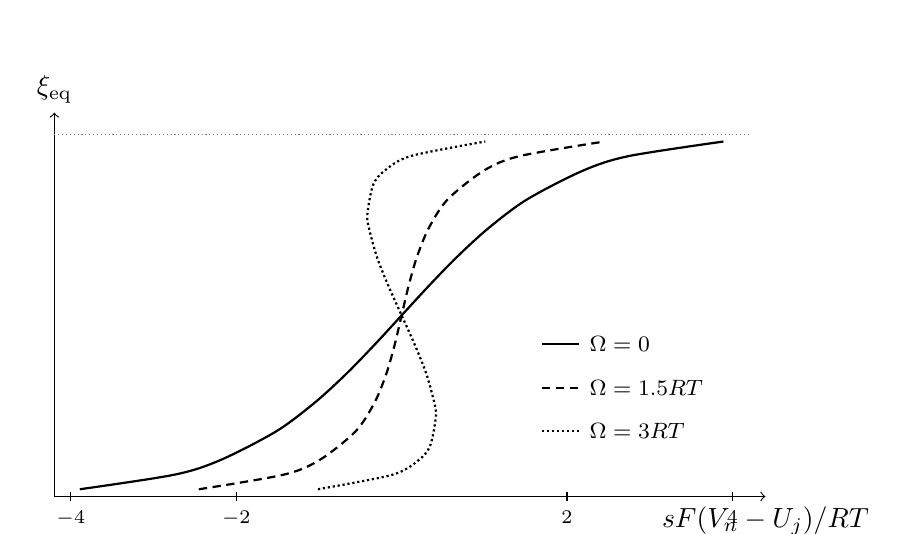
\begin{tikzpicture}[x=1.05cm,y=4.6cm]
\draw[->] (-4.2,0) -- (4.4,0) node[below] {$sF(V_n-U_j)/RT$};
\foreach \xx in {-4,-2,2,4} {\draw (\xx,0.012) -- (\xx,-0.012) node[below] {\scriptsize $\xx$};}
\draw[->] (-4.2,0) -- (-4.2,1.06) node[above] {$\xi_{\eq}$};
\draw[gray,densely dotted] (-4.2,1) -- (4.2,1);
\draw[thick] plot[smooth] coordinates {(-3.892,0.02) (-2.752,0.06) (-2.197,0.1) (-1.516,0.18) (-1.046,0.26) (-0.663,0.34) (-0.323,0.42) (0,0.5) (0.323,0.58) (0.663,0.66) (1.046,0.74) (1.516,0.82) (2.197,0.9) (2.752,0.94) (3.892,0.98)};
\draw[thick,densely dashed] plot[smooth] coordinates {(-2.452,0.02) (-1.432,0.06) (-0.997,0.1) (-0.556,0.18) (-0.326,0.26) (-0.183,0.34) (-0.083,0.42) (0,0.5) (0.083,0.58) (0.183,0.66) (0.326,0.74) (0.556,0.82) (0.997,0.9) (1.432,0.94) (2.452,0.98)};
\draw[thick,densely dotted] plot[smooth] coordinates {(-1.012,0.02) (-0.112,0.06) (0.203,0.1) (0.345,0.14) (0.414,0.22) (0.394,0.26) (0.297,0.34) (0.157,0.42) (0,0.5) (-0.157,0.58) (-0.297,0.66) (-0.394,0.74) (-0.414,0.78) (-0.345,0.86) (-0.203,0.9) (0.112,0.94) (1.012,0.98)};
\draw[thick] (1.7,0.42) -- (2.15,0.42) node[right] {\footnotesize $\Omega=0$};
\draw[thick,densely dashed] (1.7,0.30) -- (2.15,0.30) node[right] {\footnotesize $\Omega=1.5RT$};
\draw[thick,densely dotted] (1.7,0.18) -- (2.15,0.18) node[right] {\footnotesize $\Omega=3RT$};
\end{tikzpicture}
\caption{등온선~\eqref{eq:isotherm}: $\Omega=0$(실선, 폭 $RT/F$), $\Omega=1.5RT$(파선, 좁아진 단조), $\Omega=3RT>2RT$(점선, 비단조 — 한 전위에 세 $\xi$). 경계 $\Omega=2RT$, 곧 $T_{c,j}=\Omega_j/2R$.}
\label{fig:isofamily}
\end{figure}

\subsection{갈라짐의 물리 — 섞임이 손해가 되는 순간}
식~\eqref{eq:gbar} 를 $\xi=1-\theta$ 로 옮기면 기준 잔여 $-\mu^0\xi$ 와 전기 일 몫($\propto\xi$, 식~\eqref{eq:emu})이 $\xi$ 의 1차(직선) 몫이 되는데, 공통 접선 판정(식~\eqref{eq:chordtest})은 1차항에 불변이므로 이를 상수 $g_j^0$ 와 함께 떼면
\begin{equation}
g_j(\xi)=g_j^0+RT\big[\xi\ln\xi+(1-\xi)\ln(1-\xi)\big]+\Omega_j\,\xi(1-\xi)
\label{eq:gxi}
\end{equation}
이다(엔트로피 몫은 아래로 볼록; $\Omega_j>0$ 몫은 가운데를 위로). $\Omega_j$ 가 크면 가운데가 언덕, 양쪽에 골짜기 둘(그림~\ref{fig:doublewell}) — 평균 조성 $\xi$ 를 균질로 두거나 $\xi^-,\xi^+$ 로 갈라 둘 수 있고, 갈라진 상태의 평균은 두 점을 잇는 현 위에 놓인다. 옅은 쪽 분율 $f$ 의 지렛대 규칙으로
\begin{equation}
f\,\xi^-+(1-f)\,\xi^+=\xi
\quad\Rightarrow\quad
\bar g_{\text{갈라짐}}(\xi)\;=\;f\,g(\xi^-)+(1-f)\,g(\xi^+)
\label{eq:lever}
\end{equation}
(둘 다 $f$ 에 선형이라 현 위를 정확히 움직인다). 판정이 한 식으로 닫힌다:
\begin{equation}
g_j(\xi)\;>\;\bar g_{\text{갈라짐}}(\xi)
\quad\Longleftrightarrow\quad
\text{갈라지는 쪽이 이득.}
\label{eq:chordtest}
\end{equation}
이득이 끝나는 경계는 곡선에 두 점에서 동시에 접하는 공통 접선이고, 접점에서 두 기울기와 현의 기울기가 같다:
\begin{equation}
g_j'(\xi_b^-)\;=\;g_j'(\xi_b^+)
\;=\;\frac{g_j(\xi_b^+)-g_j(\xi_b^-)}{\xi_b^+-\xi_b^-}.
\label{eq:cotangent}
\end{equation}
이 두 접점 $\xi_b^\pm$ 가 \textbf{binodal(공존 조성)}. $g_j$ 가 $\xi=\tfrac12$ 대칭이라 공통 접선이 수평($g_j'=0$)이고, 아래 식~\eqref{eq:gprime} 의 $g_j'$ 에 $g_j'=0$ 을 넣으면
\begin{equation}
RT\ln\frac{\xi_b}{1-\xi_b}+\Omega_j\,(1-2\xi_b)\;=\;0
\qquad(\text{자명근 }\xi=\tfrac12\text{(언덕 꼭대기) 를 제외한 두 근 }\xi_b,\ 1-\xi_b)
\label{eq:binodal}
\end{equation}
의 두 근이 binodal 이다(수치는 아래 검산). 식~\eqref{eq:gxi} 를 미분하면 그 결과가 식~\eqref{eq:isotherm} 의 우변이다:
\begin{equation}
g_j'(\xi)\;=\;RT\ln\frac{\xi}{1-\xi}+\Omega_j\,(1-2\xi)
\;=\;sF\,(V_{\eq,j}-U_j).
\label{eq:gprime}
\end{equation}
접선 위에서 기울기가 일정 $\Rightarrow$ 갈라진 동안 평형 전위가 한 값에 머문다(\emph{평탄 전위}, plateau; 대칭 모형에서 $g'=0$ 이라 정확히 $U_j$). 좁은 $\dd V$ 에 큰 $\dd Q$ — ICA peak 의 정체가 이 접선이다. 가운데 언덕 구간은 $g''<0$ 이라 미소 요동에도 즉시 무너지고(그 경계 $g''=0$ 의 두 변곡점이 \textbf{spinodal}, 아래 식~\eqref{eq:spinodal}), binodal--spinodal 사이는 $g''>0$ 라 갈라짐이 전역 이득이나 핵생성 장벽(\S\ref{sec:rate} 의 언덕)을 넘어야 도달하는 \emph{준안정}이다 — 이 과주행이 히스테리시스의 씨앗이다(\S\ref{sec:hys}). 단상 평형은 단일 자리 운동방정식~\eqref{eq:relax} 의 정지점이나, 공존 plateau 는 갈라질 자유도를 가진 다입자 앙상블의 정지 상태로 받쳐진다 — 단일 평균장 궤적은 갈라지지 못해 준안정 가지(과주행)를 따른다.

\begin{figure}[t]
\centering
\begin{tikzpicture}[x=10cm,y=48cm]
% 영역 띠(실계산 경계): binodal 0.0707/0.9293, spinodal 0.2113/0.7887 (Omega=3RT)
\fill[gray!28] (0.2113,-0.069) rectangle (0.7887,0.0745);
\fill[gray!11] (0.0707,-0.069) rectangle (0.2113,0.0745);
\fill[gray!11] (0.7887,-0.069) rectangle (0.9293,0.0745);
\node at (0.5,0.0695) {\scriptsize 불안정($g''<0$): 즉시 갈라짐};
\node[align=center] at (0.141,0.060) {\scriptsize 준안정\\[-2pt]\scriptsize ($g''>0$)};
\node[align=center] at (0.859,0.060) {\scriptsize 준안정\\[-2pt]\scriptsize ($g''>0$)};
\node at (0.141,-0.0745) {\scriptsize 핵생성 필요};
\node at (0.5,-0.0745) {\scriptsize 핵생성 불필요(즉시)};
\node at (0.859,-0.0745) {\scriptsize 핵생성 필요};
\draw[->] (0,-0.075) -- (0,0.075) node[left] {$g_j/RT$};
\draw[->] (-0.02,0) -- (1.05,0) node[below] {$\xi$};
\foreach \xx in {0.25,0.5,0.75} {\draw (\xx,0.002) -- (\xx,-0.002) node[below] {\scriptsize $\xx$};}
\draw[thick] plot[smooth] coordinates {(0.02,-0.0392) (0.06,-0.0578) (0.1,-0.0551) (0.14,-0.0438) (0.18,-0.0286) (0.22,-0.0121) (0.26,0.0041) (0.3,0.0191) (0.34,0.0322) (0.38,0.0427) (0.42,0.0505) (0.46,0.0553) (0.5,0.0569) (0.54,0.0553) (0.58,0.0505) (0.62,0.0427) (0.66,0.0322) (0.7,0.0191) (0.74,0.0041) (0.78,-0.0121) (0.82,-0.0286) (0.86,-0.0438) (0.9,-0.0551) (0.94,-0.0578) (0.98,-0.0392)};
\draw[dashed] (0.0707,-0.0583) -- (0.9293,-0.0583) node[pos=0.5,below] {\footnotesize 가장 낮은 현(공통 접선) $=$ plateau 전위};
\fill (0.0707,-0.0583) circle (0.6pt) node[below left] {\footnotesize $\xi_b^-$};
\fill (0.9293,-0.0583) circle (0.6pt) node[below right] {\footnotesize $\xi_b^+$};
\fill (0.2113,-0.0157) circle (0.6pt) node[above left] {\footnotesize $\xi_s^-$};
\fill (0.7887,-0.0157) circle (0.6pt) node[above right] {\footnotesize $\xi_s^+$};
\end{tikzpicture}
\caption{자유에너지~\eqref{eq:gxi}($\Omega_j=3RT$; 띠 경계는 식~\eqref{eq:spinodal} 실계산값). 두 접점 $\xi_b^\pm$ 사이가 갈라짐 이득(binodal; 접선 기울기 $=$ plateau 전위, 식~\eqref{eq:gprime}). 진한 띠($g''<0$)는 즉시 무너지는 불안정(spinodal 경계), 옅은 두 띠는 준안정(핵생성 장벽 — 히스테리시스 무대), 띠 밖은 안정 단상.}
\label{fig:doublewell}
\end{figure}

식~\eqref{eq:gxi} 를 두 번 미분하면
\begin{equation}
g_j''(\xi)=\frac{RT}{\xi(1-\xi)}-2\Omega_j
\label{eq:gpp}
\end{equation}
이고, $g_j''=0$ 은 $\xi^2-\xi+RT/(2\Omega_j)=0$ — 근의 공식으로
\begin{equation}
\xi_{s,j}^\pm=\tfrac12\pm\tfrac12\,u_j,\qquad u_j\equiv\sqrt{1-\frac{2RT}{\Omega_j}}
\qquad(\Omega_j>2RT),
\label{eq:spinodal}
\end{equation}
이다($u_j$ 실수 $\Leftrightarrow\Omega_j>2RT$, 곧 $T_{c,j}=\Omega_j/2R$ 아래). 한 모수 $\Omega_j/2RT$ 가 전 영역을 가른다:
\begin{equation}
\frac{\Omega_j}{2RT}\;\begin{cases}
=0 & \text{이상 logistic}~\eqref{eq:logistic},\ w=RT/F\\[2pt]
\in(0,1] & \text{좁힘}~\eqref{eq:weff},\ w^{\eff}<RT/F\ \ (=1\text{: 임계, }w^{\eff}=0)\\[2pt]
>1 & \text{상분리}~\eqref{eq:spinodal},\ \text{plateau}+\text{히스테리시스}
\end{cases}
\label{eq:omegaaxis}
\end{equation}

\begin{verifybox}
\textbf{검산.} binodal~\eqref{eq:binodal}: $\Omega_j=3RT\Rightarrow0.0707/0.9293$($\ln(0.0707/0.9293)=-2.576=-3\times0.8586$ ✓). spinodal~\eqref{eq:spinodal}: $\tfrac12\pm\tfrac12\sqrt{1/3}=0.211/0.789$. 극한: $\Omega_j\to2RT^+$ 에서 binodal$\cdot$spinodal $\to\tfrac12$($u_j\to0$), $\Omega_j<2RT$ 면 전 구간 $g''>0$($\Omega=2RT$ 는 $\xi=\tfrac12$ 한 점만 $0$)이라 갈라짐 없음 ✓.
\end{verifybox}

% ====================================================================
\section{관측축 — 전하 보존과 내부 전위 $V_n$}\label{sec:charge}
% ====================================================================
완화 속도~\eqref{eq:kuniv}, 평형 등온선~\eqref{eq:logistic}, 일반형~\eqref{eq:isotherm} 은 이론 변수($k$, $\xi$, $V$)로 적혀 있으나 측정량은 $I(t)$$\cdot$단자 전압$\cdot$$\dd Q/\dd V$ 이므로, 이 절이 두 축을 잇는다 — 내부 전위 $V_n$ 의 출처와 관측 $\dd Q/\dd V$ 의 정체.

\subsection{전하 보존 — $V_n$ 은 풀려서 나오는 값이다}
Faraday 법칙에서 방전 전하의 패러데이 몫 $=F\times$(빠진 Li 몰수)이고, 빠진 Li 는 staging 전이 몫 $\sum_jQ_j\xi_j$ 과 배경 몫 $Q_\bg(V_n,T)$(희박 고용체$\cdot$표면/결함 자리$\cdot$전기이중층)로 교차항 없이 갈라진다. 배경은 전이보다 빨라 $V_n$ 을 준평형 추종하므로 순간 함수 $Q_\bg(V_n,T)$ 로 쓴다. 무차원 좌표 $q=\int|I|\,\dd t/Q_\cell$(적분형은 방전 가지 기준 — 충전 가지는 \S\ref{sec:master} 가 방향 부호로 처리)로 정리하면
\begin{equation}
\boxed{\;Q_\cell\,q\;=\;Q_\bg(V_n,T)\;+\;\sum_{j=1}^{N_p}Q_j\,\xi_j\;.}
\label{eq:charge}
\end{equation}
좌변은 외부 입력, 우변은 내부 상태($V_n$, $\{\xi_j\}$)의 함수다. 주어진 $\{\xi_j\}$ 에서 식~\eqref{eq:charge} 를 만족하도록 정해지는 $V_n$ 이 내부 전위 — 표에서 읽는 값이 아니라 \textbf{보존식의 해}다 \cite{mckinnon1983,newman2004}.

해의 유일성은 배경 미분용량
\begin{equation}
C_\bg\equiv\frac{\partial Q_\bg}{\partial V_n}\;>\;0
\label{eq:cbg}
\end{equation}
에서 온다. 고정된 $\{\xi_j\}$ 에서 식~\eqref{eq:charge} 우변을 $V_n$ 으로 미분하면 전이 몫이 죽고
\begin{equation}
\frac{\partial}{\partial V_n}\Big[Q_\bg(V_n,T)+\sum_jQ_j\,\xi_j\Big]_{\{\xi_j\}\ \text{고정}}
\;=\;C_\bg\;>\;0
\label{eq:unique}
\end{equation}
— 우변이 $V_n$ 단조 증가($C_\bg>0$, 배경 단상 안정성)이므로 해는 유일하고 배경 치역 안에서 존재가 보장된다. 평형($\xi_j=\xi_{\eq,j}(V_n)$)에서는 우변 기울기가 $C_\bg+\sum_jQ_j\,\dd\xi_{\eq,j}/\dd V_n$ 이고, \S\ref{sec:regsol} 의 $\Omega_j>2RT$ 비단조 구간에서 이것이 $<0$ 이 되어 한 $V_n$ 에 평형 해가 공존한다 — ``OCV $=$ 보존식의 평형 해''는 단상 유일$\cdot$상분리 구간 이력 분기의 조건부 명제(\S\ref{sec:hys})다.

\subsection{세 전위 — 내부$\cdot$측정$\cdot$구동}
측정 전위는 내부 전위에 분극이 더해진 값이다:
\begin{equation}
V_\app=V_n+s_I|I|R_n.
\label{eq:vapp}
\end{equation}
\S\ref{sec:fwdrev} 의 구동 전위 기본형은 $V_\drive=V_n$ — 계면 과전압을 내부 전위에 흡수한 lumped 근사로, 율속이 고상 재배열$\cdot$핵생성에 지배될 때 타당하다. 세 전위 $V_n$(보존식의 해)$\cdot$$V_\app$(측정)$\cdot$$V_\drive$(구동)는 지위가 다른 양이며 본 문건 전체에서 구분을 유지한다.

\subsection{관측 $\dd Q/\dd V$ — 어떤 미분인가}
$\xi_{\eq,j}$ 는 $V_n$ 의 함수(식~\eqref{eq:logistic})인데 그 $V_n$ 은 $\xi_j$ 를 입력으로 받는 보존식의 해다 — 이 고리는 미분 경로의 구분으로 닫는다. 한 순간($q$ 고정)에는 $\{\xi_j(q)\}$ 를 고정해 $V_n$ 을 풀고, 관측 $\dd Q/\dd V$ 는 궤적을 따라 보는 양이라 $\xi_j$$\cdot$$V_n$ 둘 다 $q$ 의 함수로 둔다. 보존식~\eqref{eq:charge} 양변을 $q$ 로 미분하면
\begin{equation}
Q_\cell\;=\;C_\bg\,\frac{\dd V_n}{\dd q}\;+\;\sum_jQ_j\,\frac{\dd\xi_j}{\dd q}
\label{eq:chargederiv}
\end{equation}
이고($\dd Q/\dd q=Q_\cell$), 양변을 $\dd V_n/\dd q$ 로 나누면
\begin{equation}
\frac{\dd Q}{\dd V_n}\;=\;\frac{\dd Q/\dd q}{\dd V_n/\dd q}
\;=\;C_\bg+\sum_jQ_j\,\frac{\dd\xi_j}{\dd V_n}
\label{eq:dQdV}
\end{equation}
로 닫힌다($(\dd\xi_j/\dd q)/(\dd V_n/\dd q)=\dd\xi_j/\dd V_n$ 이 궤적 연쇄율). $\xi_j$ 를 $V_n$ 의 직접 함수로 보는 것은 평형 추종 영역에 한하며, 추종이 깨지는 영역은 \S\ref{sec:lag} 가 맡는다. 이상적 plateau 의 연쇄율 발산은 ``전위 평탄 구간 $=$ peak'' 그 자체다:
\begin{equation}
\frac{\dd V_n}{\dd q}\to0
\quad\Longrightarrow\quad
\frac{\dd Q}{\dd V_n}=\frac{Q_\cell}{\dd V_n/\dd q}\to\infty.
\label{eq:plateaudiv}
\end{equation}
무한히 날카로운 이상 peak 를 유한한 모양으로 만드는 것이 다음 절부터의 일이다.

\begin{verifybox}
\textbf{Worked example.} $N_p=3$, $Q_1=Q_2=Q_3=0.3\,Q_\cell$, $\xi_1=1.00$, $\xi_2=0.55$, $\xi_3=0.02$, $q=0.5$ 에서 식~\eqref{eq:charge} 를 $Q_\bg$ 로 풀면
\begin{equation*}
Q_\bg(V_n)=Q_\cell\,q-\sum_jQ_j\xi_j
=\big[0.5-0.3\,(1.00+0.55+0.02)\big]Q_\cell
=0.029\,Q_\cell
\end{equation*}
— $C_\bg>0$ 의 단조성에 의해 이를 만족하는 $V_n$ 은 정확히 하나다(피팅 알고리즘 \S\ref{sec:master} 의 $V_{n,\OCV}(q)$ 생성도 같은 풀이 — 그림~\ref{fig:chargesolve}).
\end{verifybox}

\begin{figure}[t]
\centering
\begin{tikzpicture}[x=1.5cm,y=1cm]
\draw[->] (-3.2,0) -- (3.4,0) node[below] {\footnotesize $(V_n-V_0)/w_\bg$};
\draw[->] (-3.2,0) -- (-3.2,4.1) node[above] {\footnotesize 전하 $[Q_\cell]$};
\foreach \xx in {-2,0,2} {\draw (\xx,0.04) -- (\xx,-0.04) node[below] {\scriptsize \xx};}
\draw (-3.16,0.456) -- (-3.24,0.456) node[left] {\scriptsize 0.48};
\draw (-3.16,1.976) -- (-3.24,1.976) node[left] {\scriptsize 0.52};
\draw (-3.16,3.496) -- (-3.24,3.496) node[left] {\scriptsize 0.56};
\draw[thick] plot[smooth] coordinates {(-3,0.2942) (-2.5,0.4023) (-2,0.567) (-1.5,0.8072) (-1,1.136) (-0.5,1.5487) (0,2.014) (0.5,2.4793) (1,2.892) (1.5,3.2208) (2,3.461) (2.5,3.6257) (3,3.7338)};
\draw[thick,densely dashed] (-3.2,1.216) -- (3.2,1.216);
\fill (-0.8954,1.216) circle (1pt);
\draw[densely dotted] (-0.8954,1.216) -- (-0.8954,0);
\node[below] at (-0.8954,-0.18) {\scriptsize $V_n^{\,*}$};
\node[right] at (0.5,2.1) {\scriptsize 우변: $0.471+Q_\bg(V_n)$ — $C_\bg>0$ 라 단조};
\node[right] at (-3.0,1.444) {\scriptsize 좌변: $Q_\cell\,q=0.5$};
\end{tikzpicture}
\caption{보존식~\eqref{eq:charge} 의 $V_n$ 결정 — worked example 수치. 우변(실선)이 식~\eqref{eq:unique} 의 단조성으로 좌변(파선)과 한 번 만나는 교점 $V_n^*$($Q_\bg=0.029\,Q_\cell$)가 내부 전위다.}
\label{fig:chargesolve}
\end{figure}

% ====================================================================
\section{평형 peak 기준선}\label{sec:eqpeak}
% ====================================================================
평형 등온선~\eqref{eq:logistic} 과 관측식~\eqref{eq:dQdV} 에서 평형 peak 의 위치$\cdot$폭$\cdot$높이를 읽는다 — 이 기준선이 있어야 전류가 흐를 때의 변화를 이탈로 읽는다.

\subsection{logistic 의 미분 — 종 모양}
평형 추종이면 관측식~\eqref{eq:dQdV} 의 $\dd\xi_j/\dd V_n$ 에 평형 기울기가 들어간다. 식~\eqref{eq:logistic} 을 $z\equiv s(V_n-U_j)/w_j$ 로 치환해 $\xi_{\eq}=(1+e^{-z})^{-1}$ 를 미분하면
\begin{equation}
\frac{\dd\xi_{\eq}}{\dd z}
=\frac{e^{-z}}{(1+e^{-z})^{2}}
=\underbrace{\frac{1}{1+e^{-z}}}_{\xi_{\eq}}\cdot
\underbrace{\frac{e^{-z}}{1+e^{-z}}}_{1-\xi_{\eq}}
=\xi_{\eq}\,(1-\xi_{\eq})
\label{eq:belliden}
\end{equation}
이고, 연쇄율 $\dd z/\dd V_n=s/w_j$ 를 곱하면
\begin{equation}
\frac{\dd\xi_{\eq,j}}{\dd V_n}\;=\;\frac{s\,\xi_{\eq,j}(1-\xi_{\eq,j})}{w_j}.
\label{eq:dxidV}
\end{equation}
식~\eqref{eq:dxidV} 를 관측식~\eqref{eq:dQdV} 에 넣으면 — $\xi(1-\xi)$ 는 $\xi=\tfrac12$ 에서 최대 $\tfrac14$ 인 종 모양 — peak 의 세 양이 읽힌다:
\begin{equation}
\boxed{\;V_\peak=U_j(T),\qquad
\Big(\frac{\dd Q}{\dd V_n}\Big)^{\text{net}}_{\max}=\frac{Q_j}{4w_j},\qquad
\int\Big(\frac{\dd Q}{\dd V_n}-C_\bg\Big)\dd V_n=Q_j\;.}
\label{eq:eqpeak}
\end{equation}
위치 $=$ 전이 중심 $U_j$, 순높이 $=Q_j/(4w_j)$(평형 peak 은 방향 불변 — 충방전 방향은 통합형 \S\ref{sec:master} 의 $\sigma_d$ 가 처리), 배경 차감 면적 $=Q_j$($\int_0^1\dd\xi=1$ — 분리 peak 기준, 겹침 합산은 \S\ref{sec:overlap}). 너비는 별도 지표 없이 면적/높이 비로 읽으며, $w_j$ 는 이상 극한에서 $RT/F$($25.7$ mV, $25^\circ$C), 상호작용 시 식~\eqref{eq:weff} 의 $w^{\eff}$ 로 좁아진다.

\begin{verifybox}
\textbf{수치 재현.} $Q_j=0.3\,Q_\cell$, $w_j=25.7$ mV 면 순높이 $Q_j/(4w_j)=0.3/(4\times0.0257)\approx2.9\,Q_\cell/\mathrm V$, 배경 차감 면적 $=0.3\,Q_\cell$. 극한 — $w\to0$ 에서 높이 발산$\cdot$면적 불변(이상 plateau ICA 선), $T$ 상승 시 $w\propto T$ 라 종이 낮고 넓어진다(면적 보존).
\end{verifybox}

\subsection{온도가 기준선을 움직이는 두 길}
\emph{폭과 높이.} $w_j\propto T$ 이므로 저온일수록 평형 peak 는 좁고 높다(면적 보존). 관측은 정반대(저온에서 넓고 낮다)이며, 그 역전이 동역학 꼬리의 증거다.

\emph{위치.} 식~\eqref{eq:eqcond} 의 $\Delta G_j=-sFU_j$ 와 Gibbs 항등식 $\partial\Delta G/\partial T|_P=-\Delta S$ 를 잇으면
\begin{equation}
\Delta G_j=-sF\,U_j,\qquad
\frac{\partial\Delta G_j}{\partial T}=-\Delta S_j
\quad\Longrightarrow\quad
\frac{\partial U_j}{\partial T}=\frac{\Delta S_j}{sF}.
\label{eq:dUdT}
\end{equation}
$\Delta S_j$ 는 삽입 \emph{반응} 엔트로피로 활성화 엔트로피 $\Delta S_{a,j}$ 와 다르다 \cite{reynier2004}. $|\Delta S_j|\sim$ 수 J/(mol\,K) 라 $|\partial U_j/\partial T|\sim0.01$--$0.1$ mV/K — $30$ K 창에서 $0.3$--$3$ mV, 다온도 피팅에서 온도마다 $U_j(T)$ 를 따로 읽어야 하는 이유다(\S\ref{sec:master}).

\emph{상분리 영역.} $\Omega_j>2RT$ 전이의 평형 기여는 종이 아니라 공통 접선 plateau(\S\ref{sec:regsol}) — 이상적으로 무한히 날카로운 선 — 이고, 실측의 유한 폭은 평형이 아니라 broadening(입자 분포$\cdot$동역학) 기원이며 처리는 \S\ref{sec:hyspeak} 가 한다.

% ====================================================================
\section{C-rate 가지 — 지연과 꼬리}\label{sec:lag}
% ====================================================================
근본식의 첫 가지 — \S\ref{sec:rate} 의 C-rate 경쟁(전류 요구 vs 식~\eqref{eq:eyring} 공급)이 관측 peak 의 꼬리가 된다. 경쟁을 보편 미분방정식으로 적고 닫힌 일반해를 구한 뒤, 상승부와 꼬리를 같은 해의 두 극한으로 읽는다.

\subsection{측정축으로 옮긴 운동방정식}
정전류 방전에서 $\dd q/\dd t=|I|/Q_\cell$ 이다. 운동방정식~\eqref{eq:relax} 을 $\dd q/\dd t$ 로 나누면(기본형 $\xi_{\sstat}=\xi_{\eq}$)
\begin{equation}
\frac{\dd\xi_j}{\dd q}
=\frac{\dd\xi_j/\dd t}{\dd q/\dd t}
=\frac{Q_\cell\,k_j}{|I|}\,\big(\xi_{\eq,j}-\xi_j\big).
\label{eq:relaxq}
\end{equation}
지연 $r_j\equiv\xi_{\eq,j}-\xi_j$(위첨자 없음 — 속도 $r_j^\pm$ 와 다른 양)의 변화율 $\dd r_j/\dd q=\dd\xi_{\eq,j}/\dd q-\dd\xi_j/\dd q$ 에 식~\eqref{eq:relaxq} 를 넣으면, 영역 제한 없이 성립하는 보편 방정식이 나온다:
\begin{equation}
\frac{\dd r_j}{\dd q}\;=\;\frac{\dd\xi_{\eq,j}}{\dd q}\;-\;\frac{r_j}{L_{q,j}},\qquad
\boxed{\;L_{q,j}=\frac{|I|}{Q_\cell\,k_j}\;.}
\label{eq:Lq}
\end{equation}
첫 항은 평형 목표 이동의 지연 \emph{공급}, 둘째 항은 완화의 지연 \emph{소거}다. $L_{q,j}$ 는 요구($|I|/Q_\cell$)/공급($k_j$, 식~\eqref{eq:eyring}) 비 그 자체로, 근본식 세 인자가 전부 이 한 양을 통해 꼬리로 들어온다. 꼬리 영역($\mathcal A_j\gtrsim$ 수 $RT$)에서 $k_j\simeq r_j^+$ 로 읽으며, 괄호 인자 $(1+e^{-\mathcal A_j/RT})$ 가 살아 있는 전이대는 \S\ref{sec:potbranch} 가 정리한다.

\subsection{일반해 — 지수 기억}
식~\eqref{eq:Lq} 는 1계 선형 ODE 라 적분인자 $e^{q/L_{q,j}}$ 로 닫힌 해를 갖는다($L_{q,j}$ 가 적분 구간에서 천천히 변한다는 가정 — 정량 조건은 아래 검산). 곱의 미분이 좌변을 완전 미분으로 묶고, 식~\eqref{eq:Lq} 를 이항해 대입하면
\begin{equation}
\frac{\dd}{\dd q}\Big(r_j\,e^{q/L_{q,j}}\Big)
=e^{q/L_{q,j}}\Big(\frac{\dd r_j}{\dd q}+\frac{r_j}{L_{q,j}}\Big)
=e^{q/L_{q,j}}\,\frac{\dd\xi_{\eq,j}}{\dd q}.
\label{eq:intfactor}
\end{equation}
$q_0$ 부터 $q$ 까지 적분하면 좌변은 양 끝값의 차만 남고
\begin{equation}
r_j(q)\,e^{q/L_{q,j}}-r_j(q_0)\,e^{q_0/L_{q,j}}
=\int_{q_0}^{q}e^{q'/L_{q,j}}\,\frac{\dd\xi_{\eq,j}}{\dd q'}\,\dd q',
\label{eq:intfacint}
\end{equation}
$e^{-q/L_{q,j}}$ 를 곱해 $r_j(q)$ 를 꺼내면 닫힌 일반해가 나온다:
\begin{equation}
r_j(q)\;=\;r_j(q_0)\,e^{-(q-q_0)/L_{q,j}}
\;+\;\int_{q_0}^{q}e^{-(q-q')/L_{q,j}}\,\frac{\dd\xi_{\eq,j}}{\dd q'}\,\dd q'.
\label{eq:memory}
\end{equation}
지연은 초기 지연의 지수 감쇠 $+$ 과거 목표 변화율을 지수 커널로 가중한 \emph{기억}의 합이고, 둘째 몫은 합성곱이다:
\begin{equation}
r_j(q)\Big|_{r_j(q_0)=0}
=\big(K*\tfrac{\dd\xi_{\eq,j}}{\dd q}\big)(q),
\qquad K(\Delta q)=e^{-\Delta q/L_{q,j}}\ \ (\Delta q\ge0).
\label{eq:conv}
\end{equation}
계는 용량축에서 길이 $L_{q,j}$ 만큼의 최근 과거만 기억한다(그림~\ref{fig:kernel}). 수치 — $0.1$C, $k_j=10^{-3}\ \mathrm{s^{-1}}$ 이면 $L_{q,j}=(0.1/3600)/10^{-3}\approx0.028$(방전의 $3\%$); 저온으로 $k_j$ 가 $12$배 느리면 $L_{q,j}\approx0.33$(전이 하나를 통째로 덮는 길이).

\begin{figure}[t]
\centering
\begin{tikzpicture}[x=0.58cm,y=17cm]
\draw[->] (-4,0) -- (10.9,0) node[below] {$(q-q_{\peak})/(\text{상승부 폭})$};
\foreach \xx in {-2,0,2,4,6,8} {\draw (\xx,0.006) -- (\xx,-0.006) node[below] {\scriptsize $\xx$};}
\draw[->] (-4,0) -- (-4,0.33) node[above] {\footnotesize (임의 단위)};
\draw[densely dotted,thick] plot[smooth] coordinates {(-4,0.0177) (-3,0.0452) (-2.5,0.0701) (-2,0.105) (-1.5,0.1491) (-1,0.1966) (-0.5,0.235) (0,0.25) (0.5,0.235) (1,0.1966) (1.5,0.1491) (2,0.105) (2.5,0.0701) (3,0.0452) (3.5,0.0285) (4,0.0177) (5,0.0066) (6,0.0025) (7,0.0009) (8,0.0003) (10,0.0)};
\draw[thick] plot[smooth] coordinates {(-4,0.0087) (-3,0.027) (-2.5,0.0438) (-2,0.0686) (-1.5,0.1034) (-1,0.1482) (-0.5,0.1989) (0,0.2469) (0.5,0.2808) (1,0.2932) (1.5,0.2831) (2,0.2561) (2.5,0.2199) (3,0.1815) (3.5,0.1452) (4,0.1136) (5,0.0661) (6,0.0369) (7,0.02) (8,0.0107) (9,0.0056) (10,0.0029)};
\draw[densely dashed,thick] plot[smooth] coordinates {(-4,0.0041) (-3,0.0106) (-2.5,0.0167) (-2,0.0254) (-1.5,0.0370) (-1,0.0506) (-0.5,0.0637) (0,0.0721) (0.5,0.0727) (1,0.0653) (1.5,0.0529) (2,0.0393) (2.5,0.0274) (3,0.0182) (3.5,0.0117) (4,0.0074) (5,0.0028) (6,0.0011) (7,0.0004) (8,0.0001) (10,0.0)};
\node at (-2.9,0.225) {\footnotesize 원천 $\dd\xi_{\eq}/\dd q$};
\node at (5.7,0.215) {\footnotesize 지연 $r_j$($L_q=1.5\times$폭)};
\node at (5.1,0.062) {\scriptsize 추종 $r_j$($L_q=0.3\times$폭)};
\draw[->,gray] (3.95,0.055) -- (2.95,0.024);
\draw[<->,gray] (1,0.318) -- (2.5,0.318) node[pos=0.5,above] {\footnotesize $\sim L_{q,j}$};
\end{tikzpicture}
\caption{일반해~\eqref{eq:memory} 의 기억 거동(두 케이스). 점선 $=$ 원천 $\dd\xi_{\eq}/\dd q$. 파선($L_q=0.3\times$폭) $=$ 식~\eqref{eq:risefollow} 의 축소 추종(정점 $\approx L_q\times$원천). 실선($L_q=1.5\times$폭) $=$ 기억이 상승부를 덮어 정점이 늦고 높으며, 원천 포화 후 식~\eqref{eq:rsol} 의 지수 감쇠로 넘어감 — 상승부(추종)$\cdot$꼬리(지수 기억) 두 극한이 한 해의 두 얼굴.}
\label{fig:kernel}
\end{figure}

\subsection{두 극한 — 상승부와 꼬리}
\emph{극한 (i): 상승부.} 한 기억 길이 안에서 $\dd\xi_{\eq}/\dd q'$ 가 거의 일정하면 일반해~\eqref{eq:memory} 의 적분에서 그 인자를 현재값으로 꺼낼 수 있고(초기 지연 항은 $q-q_0\gg L_q$ 에서 사멸), 남는 지수 커널 적분은 닫힌 꼴이다:
\begin{equation}
\int_{q_0}^{q}e^{-(q-q')/L_{q,j}}\,\dd q'
=L_{q,j}\Big[1-e^{-(q-q_0)/L_{q,j}}\Big]
\;\xrightarrow{\ q-q_0\gg L_{q,j}\ }\;L_{q,j}.
\label{eq:kernelint}
\end{equation}
따라서
\begin{equation}
r_j(q)\;\simeq\;L_{q,j}\,\frac{\dd\xi_{\eq,j}}{\dd q}\bigg|_{q}\;+\;O(L_{q,j}^2)
\label{eq:risefollow}
\end{equation}
— 지연이 목표 변화율에 비례하는 소량이다($O(L^2)$ 는 식~\eqref{eq:kernelint} 적분의 부분적분 잔여 $L_{q,j}^2\,\dd^2\xi_{\eq}/\dd q^2$). 빠른 동역학 극한($k\to\infty$, $L_q\to0$)에서 $r\to0$, 평형 추종이 회복된다 — 상승부 관측이 평형 peak 기준선에 지배되는 근거.

\emph{극한 (ii): 꼬리.} peak 를 지나 목표가 포화하면 원천이 꺼진다. 꼬리 시작점 $q_a=$``원천 $\dd\xi_{\eq,j}/\dd q$ 가 정점의 일정 분율(예 $5\%$) 이하로 떨어지는 첫 좌표''(컷은 데이터셋 공통 고정 — \S\ref{sec:master})에서 일반해~\eqref{eq:memory} 를 다시 시작하면, 원천이 꺼져($\dd\xi_{\eq}/\dd q'\simeq0$, $q'>q_a$) 기억 적분이 사라지고 초기 지연 감쇠만 남는다:
\begin{equation}
r_j(q)\;=\;r_{a,j}\,\exp\!\Big[-\frac{q-q_a}{L_{q,j}}\Big]\qquad(q\ge q_a),\qquad
r_{a,j}\equiv r_j(q_a).
\label{eq:rsol}
\end{equation}
지연이 길이 $L_{q,j}$ 로 지수 감쇠한다(컷 잔여 $\le5\%$ 처리와 $\chi$-편향 정량은 \S\ref{sec:master} (3$'$)). 꼬리에서 목표가 포화해 $\xi_j=\xi_{\eq,j}-r_j$ 의 미분에 지연 몫만 남고, 식~\eqref{eq:rsol} 미분 시 지수에서 $-1/L_{q,j}$ 가 내려와 음부호와 상쇄되어
\begin{equation}
\frac{\dd\xi_j}{\dd q}
=\underbrace{\frac{\dd\xi_{\eq,j}}{\dd q}}_{\simeq\,0\ (\text{포화})}-\;\frac{\dd r_j}{\dd q}
\;\simeq\;\frac{r_{a,j}}{L_{q,j}}\,\exp\!\Big[-\frac{q-q_a}{L_{q,j}}\Big]
\label{eq:tailrate}
\end{equation}
— 같은 지수형, 진폭 $r_{a,j}/L_{q,j}$. 전압축으로 옮기면 — 관측 꼬리 몫은 연쇄율(\S\ref{sec:charge})로 $Q_j(\dd\xi_j/\dd q)$ 를 $\dd V_n/\dd q$ 로 나눈 것이고, post-peak 국소 기울기로 $q-q_a$ 를 ($V_n-V_{a,j}$ 를 $|\dd V_n/\dd q|_{q_a}$ 로 나눈 값) 식~\eqref{eq:tailrate} 지수에 대입하면
\begin{equation}
\frac{\dd Q}{\dd V_n}\Big|_{\text{tail}}
=\frac{Q_j\,r_{a,j}}{L_{V,j}}\,
\exp\!\Big[-\frac{V_n-V_{a,j}}{L_{V,j}}\Big]\quad\big(s(V_n-V_{a,j})\ge0\big),\qquad
L_{V,j}=\Big|\frac{\dd V_n}{\dd q}\Big|_{q_a}L_{q,j}
\label{eq:tail}
\end{equation}
— 진폭까지 닫힌 꼴이다. 분자 $1/L_{q,j}$ 와 분모 $\dd V_n/\dd q$ 가 전압축 길이 $L_{V,j}$ 로 묶였고, 분포 일반형(\S\ref{sec:tempbranch})$\cdot$실무 피팅형(\S\ref{sec:synth})의 꼬리 진폭 $r_a/L_V$ 가 이 식이다. 꼬리는 단방향(방전 진행 방향)이며($s=+1$ 기준), 충전 가지의 거울상 감쇠는 통합형(\S\ref{sec:master})이 $\sigma_d$ 로 처리한다.

\begin{verifybox}
\textbf{상수 $L_q$ 의 정량 조건.} 일반해는 $L_{q,j}$ 를 적분 밖으로 꺼냈다 — 유효 조건은 한 감쇠 길이 동안 $\ln L_q$ 변화가 작다는 것, 전위 의존(\S\ref{sec:potbranch})으로 $(\chi F/RT)\,L_{V,j}\ll1$. 전형값($\chi=0.5$, $L_V=5$ mV, $25^\circ$C)으로 $\approx0.1$ — 성립하나 경계적이며 꼬리가 길어지면 위반된다. 위반의 지문 $=$ 후미 \emph{가속}(꼬리가 깊어질수록 $L_q$ 감소 → 반로그에서 현 \emph{위로} 부풂); \S\ref{sec:tempbranch} 분포 늘어짐(현 \emph{아래로} 처짐)과 곡률 부호가 반대라 잔차로 구별되고, 처방은 $\mathcal A_j(V)$ 드리프트를 살리는 sub-window 국소 $L_V$ 가 $\chi$ 회귀로 흡수(\S\ref{sec:master}), 기울기 $|\dd V_n/\dd q|$ 드리프트도 같은 처방이 받는다.
꼬리 면적 — $\int_{V_{a}}^{\infty}(\dd Q/\dd V_n)|_{\text{tail}}\,\dd V_n
=(Q_jr_{a,j}/L_{V,j})\cdot L_{V,j}=Q_j\,r_{a,j}$: 꼬리 운반 전하 $=$ 잔류 지연 몫(빠른 완화 극한 $r_a\to0$ 에서 꼬리 면적째 소멸 — 평형 복귀).
차원 — $L_{q,j}=[\mathrm{C/s}]/([\mathrm C][\mathrm{s^{-1}}])=$ 무차원 ✓.
\end{verifybox}

% ====================================================================
\section{전위 가지 — 유효 장벽}\label{sec:potbranch}
% ====================================================================
\S\ref{sec:fwdrev} 의 식~\eqref{eq:bv}(전위가 정$\cdot$역 장벽을 비대칭으로 옮김)을 앞 절의 꼬리 길이 $L_{q,j}$~\eqref{eq:Lq} 에 새기는 절이다.

\subsection{유효 장벽과 forward 극한}
꼬리는 $\mathcal A_j>0$ 이라 정방향 우세다. \S\ref{sec:fwdrev} 의 보편형 $k_j=r_j^+(1+e^{-\mathcal A_j/RT})$ 에서 역방향 몫 $e^{-\mathcal A_j/RT}$ 은 $\mathcal A_j=RT$ 에서 $37\%$, $3RT$ 에서 $5\%$ 이므로
\begin{equation*}
e^{-\mathcal A_j/RT}\big|_{\mathcal A_j=RT}\approx0.37,\qquad
e^{-\mathcal A_j/RT}\big|_{\mathcal A_j=3RT}\approx0.05
\quad\Rightarrow\quad k_j\simeq r_j^+\ (\mathcal A_j\gtrsim3RT).
\end{equation*}
역방향 몫을 버린 forward 극한이 정확하므로:
\begin{equation}
\boxed{\;\Delta G_{\eff,j}=\Delta G_{a,j}-\chi\,\mathcal A_j,\qquad
k_j\simeq k_0\,\exp\!\Big[-\frac{\Delta G_{a,j}-\chi\mathcal A_j}{RT}\Big]
\quad(\mathcal A_j\gtrsim3RT)\;.}
\label{eq:keff}
\end{equation}
근본식~\eqref{eq:eyring} 의 장벽 자리에 $\Delta G_{\eff}$ 가 앉은 것 — 전위는 평형 목적지($U_j$의 몫)는 옮기지 않고 속도만 바꾼다. 전이대 $RT\lesssim\mathcal A_j\lesssim3RT$ 에서는 보편형 괄호 인자를 그대로 곱한다(전위만의 함수라 모든 입자 공통 — \S\ref{sec:tempbranch} 의 분포 적분 \emph{밖}; 컷 처리는 \S\ref{sec:master} M3).

\subsection{꼬리 길이의 전위 의존}
식~\eqref{eq:keff} 를 식~\eqref{eq:Lq} 에 넣으면 $L_{q,j}\propto1/k_j$. 임의 절단 대신 직렬 율속 합성으로 일반화하면($k_{j,\lim}$ 은 전위 무관):
\begin{equation*}
\frac1{k_j^{\eff}}=\frac1{k_j}+\frac1{k_{j,\lim}},\qquad
L_{q,j}\propto\frac1{k_j^{\eff}}.
\end{equation*}
식~\eqref{eq:keff} 에 로그를 취하면 $\ln k_j=\ln k_0-(\Delta G_{a,j}-\chi\mathcal A_j)/RT$ 이고, $V_\drive$ 의존은 $\mathcal A_j=sF(V_\drive-U_j)$ 뿐이라
\begin{equation}
\frac{\partial\ln k_j}{\partial V_\drive}
=\frac{\chi}{RT}\,\frac{\partial\mathcal A_j}{\partial V_\drive}
=\frac{\chi sF}{RT}.
\label{eq:dlnk}
\end{equation}
위 직렬 합성 $\ln k_j^{\eff}=-\ln[1/k_j+1/k_{j,\lim}]$ 을 $V_\drive$ 로 미분하면 전위 의존이 있는 $1/k_j$ 항만 살아
\begin{equation}
\frac{\partial\ln k_j^{\eff}}{\partial V_\drive}
=\frac{1/k_j}{1/k_j+1/k_{j,\lim}}\,\frac{\partial\ln k_j}{\partial V_\drive}
=\frac{k_{j,\lim}}{k_j+k_{j,\lim}}\,\frac{\chi sF}{RT}
\label{eq:dlnkeff}
\end{equation}
($\partial(1/k_j)/\partial V_\drive=-(1/k_j)\,\partial\ln k_j/\partial V_\drive$ 를 넣어 두 음부호가 상쇄, 둘째 등식은 분자$\cdot$분모에 $k_jk_{j,\lim}$ 을 곱한 것). $L_{q,j}\propto1/k_j^{\eff}$ 의 로그 미분은 식~\eqref{eq:dlnkeff} 의 부호 반전이므로
\begin{equation}
\frac{\partial\ln L_{q,j}}{\partial V_\drive}
\;=\;-\,\frac{k_{j,\lim}}{k_j+k_{j,\lim}}\,\frac{\chi sF}{RT}\;\le\;0\quad(s=+1).
\label{eq:LqV}
\end{equation}
구동이 깊을수록 꼬리가 짧아진다 — ``전위$\uparrow\Rightarrow$꼬리$\downarrow$'' 가 닫혔다. 앞 인자는 $k_{j,\lim}\to\infty$ 활성화 지배 극한에서 $1$ 로(기울기 $-\chi sF/RT$), 유한 공율속이면 기울기가 죽지만 부호 유지. 등온 기울기에서 $\chi$ 와 감쇠 인자가 함께 퇴화하므로 식별 사슬은 활성화 지배 확인(\S\ref{sec:master} S0) 위에서만 돈다 — 활성화 지배 여부는 측정으로 판정(\S\ref{sec:falsify} 수송 진단).

\begin{boundbox}
\textbf{선형 근사의 한계.} $-\chi\mathcal A$ 는 소구동력 1차 근사이고 Marcus 포물면 2차 항은 $\sim\mathcal A/2\lambda$ 로 들어오므로 \cite{marcus1956}, 작동 창은
\begin{equation*}
3RT\;\lesssim\;\mathcal A_j\;\ll\;\lambda
\qquad(\text{좌: forward 극한}~\eqref{eq:keff},\ \text{우: 선형 근사})
\end{equation*}
삽입 상전이에서 $\lambda$(용매$\cdot$격자 재구성)는 수십 kJ/mol — $RT\approx2.5$ kJ/mol 의 십수 배 이상 — 라 창이 넉넉하다.
\end{boundbox}

% ====================================================================
\section{온도 가지 — Arrhenius 와 입자 분포}\label{sec:tempbranch}
% ====================================================================
온도는 근본식~\eqref{eq:eyring} 지수 분모에 직접 앉는다. 이 절은 꼬리 길이에서 활성화 엔탈피를 뽑는 Arrhenius 회귀와, 장벽 분포가 온도와 결합해 꼬리를 늘어뜨리는 방식을 닫는다.

\subsection{Arrhenius 회귀 — 엔탈피만 기울기에 남기기}
식~\eqref{eq:Lq} 에 식~\eqref{eq:keff} 를 넣고 $k_0=k_BT/h$(식~\eqref{eq:eyring})를 쓰면
\begin{equation}
L_{q,j}=\frac{|I|}{Q_\cell\,k_j}
\simeq\frac{|I|}{Q_\cell}\cdot\frac{h}{k_BT}\,
\exp\!\Big[\frac{\Delta G_{a,j}-\chi\mathcal A_j}{RT}\Big]
=\frac{T_*}{T}\,\exp\!\Big[\frac{\Delta G_{a,j}-\chi\mathcal A_j}{RT}\Big],
\qquad T_*\equiv\frac{|I|\,h}{Q_\cell\,k_B}
\label{eq:LqT}
\end{equation}
($T_*$ 는 로그 무차원화 특성 온도; 지수가 양수, 곧 $\Delta G_{\eff}>0$ 인 것은 작동 창 $\mathcal A\ll\lambda$(\S\ref{sec:potbranch})가 담보). 로그를 취하고 $\Delta G_{a,j}=\Delta H_{a,j}-T\Delta S_{a,j}$ 로 갈라 적으면
\begin{equation}
\ln L_{q,j}\;=\;\ln\frac{T_*}{T}\;+\;\frac{\Delta H_{a,j}-\chi\mathcal A_j}{RT}
\;-\;\frac{\Delta S_{a,j}}{R}.
\label{eq:lnLq}
\end{equation}
$1/T$ 계수는 $\Delta H_{a,j}$ 와 $\chi\mathcal A_j$ 뿐이고 $-\Delta S_{a,j}/R$ 는 온도 무관 절편이다. 로그 인자 $\ln(T_*/T)$ 와 기지 구동항 $\chi\mathcal A_j/RT$ 를 좌변으로 이항하고 전체 부호를 뒤집으면
\begin{equation}
y(T)\;\equiv\;\ln\frac{T_*}{L_{q,j}\,T}-\frac{\chi\,\mathcal A_j(T)}{RT}
\;=\;-\frac{\Delta H_{a,j}}{R}\cdot\frac1T\;+\;\frac{\Delta S_{a,j}}{R}
\label{eq:ydef}
\end{equation}
— $1/T$ 에 순수 선형인 측정량이다. 따라서(구동항 평가점은 전 온도 공통 SOC — \S\ref{sec:master} S4):
\begin{equation}
\boxed{\;y(T)\text{ 를 }\tfrac1T\text{ 로 회귀}\;\Rightarrow\;
\text{기울기}=-\frac{\Delta H_{a,j}}{R},\qquad
\text{절편}=+\frac{\Delta S_{a,j}}{R}\ \text{(결합값)}\;.}
\label{eq:arrhenius}
\end{equation}

\begin{figure}[t]
\centering
\begin{tikzpicture}[x=1cm,y=1cm]
\draw[->] (-0.2,0) -- (6.6,0) node[below] {\footnotesize $1000/T$ [1/K]};
\draw[->] (-0.2,0) -- (-0.2,3.4) node[above] {\footnotesize $y$(무차원)};
\foreach \xx/\lab in {1.6/3.2,4.8/3.4} {\draw (\xx,0.04) -- (\xx,-0.04) node[below] {\scriptsize \lab};}
\foreach \yy/\lab in {0.42/-4.5,1.47/-3.5} {\draw (-0.16,\yy) -- (-0.24,\yy) node[left] {\scriptsize \lab};}
\draw[thick] (0.6912,1.8669) -- (5.9264,0.21315);
\fill (5.9264,0.21315) circle (1.2pt); \fill (4.4272,0.6867) circle (1.2pt); \fill (0.6912,1.8669) circle (1.2pt);
\draw[gray] (0.6912,2.9883) -- (4.4272,1.9698) -- (5.9264,1.55925);
\draw[gray] (5.9264,1.55925) circle (1.2pt); \draw[gray] (4.4272,1.9698) circle (1.2pt); \draw[gray] (0.6912,2.9883) circle (1.2pt);
\node[below right] at (3.4,0.5) {\scriptsize $y(T)$~\eqref{eq:ydef}: 기울기 $-\Delta H_a/R$};
\node[above left,gray] at (5.4,2.55) {\scriptsize 보정 전($\chi\mathcal A$ 미제거): 기울기 오염};
\node[below] at (3.1,-0.45) {\scriptsize $45^\circ$C $\leftarrow$ \quad\quad $\to$ $15^\circ$C};
\end{tikzpicture}
\caption{Arrhenius 회귀~\eqref{eq:arrhenius}($\Delta H_a=40$ kJ/mol, 절편 $12$, 세 온도 $15/23/45^\circ$C). 검정: 보정된 $y(T)$~\eqref{eq:ydef} — $1/T$ 선형, 기울기 $-\Delta H_a/R$. 회색: 구동항 $\chi\mathcal A_j/RT$ 미제거 — offset 이 온도마다 달라 기울기 오염. S4 가 $\chi$ 를 먼저 닫는 이유(\S\ref{sec:master}).}
\label{fig:arrplot}
\end{figure}

\begin{verifybox}
\textbf{특수 케이스 회수.} $\chi\mathcal A_j\to0$ 이면 $y=\ln[T_*/(L_{q,j}T)]$ — 고전 Arrhenius 회귀로 환원. 수치: $\Delta H_a=40$ kJ/mol, $15\to45^\circ$C 는 $\Delta(1/T)=3.27\times10^{-4}\ \mathrm{K^{-1}}$ 이라 $\Delta y=(\Delta H_a/R)\,\Delta(1/T)\approx1.57$ — 그림~\ref{fig:arrplot} 직선 낙차이고 $\Delta H_a$ 상대오차 어림 $\approx\delta y/1.57$.
\end{verifybox}

구동항 보정용 $\chi$ 는 전위 가지(\S\ref{sec:potbranch})에서 \emph{먼저} 닫아 기지값으로 넣어(그림~\ref{fig:arrplot}) ``$\chi$/$\Delta H_a$ 공선형''을 끊는다(피팅 단계 설계 \S\ref{sec:master} 가 이 순서). $\Delta S_{a,j}$ 는 prefactor 결합 절편으로만 나와 단독 비식별(절대값은 prefactor 에 묻고 의존성만 — \S\ref{sec:rate} 전략). 부호 주의: $y$ 회귀 절편은 $+\Delta S_{a,j}/R$, \S\ref{sec:master} M3 의 $b_j=-\Delta S_{a,j}/R$ 는 그 부호 반전($b_j=-$절편). 절편 분리는 $k_0$ 흡수 $O(1)$ 인자$\cdot$활동도 몫의 측정창 내 온도 무관을 요구(\S\ref{sec:master} 울타리 ③).

\subsection{입자 분포 — 같은 온도가 산포를 키운다}
실 전극은 입자 집단이라 활성화 장벽이 분포를 이룬다. 장벽 $G$($\equiv\Delta G_{a}$ 축약 — 이 절 한정, Gibbs 함수 아님)의 용량-분율 밀도 $\rho_G(G)$ 는 $\int\rho_G\,\dd G=1$ 정규화이고, 각 집단은 $L_q(G)\propto e^{(G-\chi\mathcal A)/RT}$ 를 갖는다. 길이의 로그가 장벽에 선형($\ln L_q=\text{const}+G/RT$)이므로
\begin{equation*}
\frac{\partial\ln L_q}{\partial G}=\frac1{RT},
\end{equation*}
선형 전파로 장벽 표준편차 $\sigma_G$ 가
\begin{equation}
\sigma_{\ln L}\;=\;\frac{\sigma_G}{RT}
\label{eq:varprop}
\end{equation}
처럼 $1/RT$ 배 전파된다 — 저온일수록 길이 산포가 커진다($\sigma_G=5$ kJ/mol: $25^\circ$C 에서 $\sigma_{\ln L}\approx2.0$, $-15^\circ$C 에서 $2.3$; 로그 폭 $2$ 는 중앙값의 $e^{\pm2}$, 양끝 간 쉰다섯 배). 관측 꼬리는 집단별 지수 꼬리~\eqref{eq:tail} 의 용량-분율 가중 합이다:
\begin{equation}
\frac{\dd Q}{\dd V_n}\Big|_{\text{tail}}
=Q_j\!\int_0^\infty\!\rho_G(G)\,\frac{r_a(G)}{L_V(G)}\,
e^{-(V_n-V_a)/L_V(G)}\,\dd G\qquad\big(s(V_n-V_a)\ge0\big).
\label{eq:superpose}
\end{equation}
분포가 한 값으로 좁아지는 극한에서 \S\ref{sec:lag} 단일지수로 정확히 환원된다:
\begin{equation}
\rho_G\to\delta(G-\bar G):\quad
\frac{\dd Q}{\dd V_n}\Big|_{\text{tail}}
\;\to\;\frac{Q_j\,r_a(\bar G)}{L_V(\bar G)}\,e^{-(V_n-V_{a})/L_V(\bar G)}
\;=\;\text{식}~\eqref{eq:tail}
\label{eq:deltareduce}
\end{equation}(전이대 컷 괄호 인자는 \S\ref{sec:potbranch} 대로 적분 \emph{밖}의 공통 인자 — 분포 비흡수). 분포가 넓으면 빠른 집단이 먼저 죽고 느린 집단이 꼬리를 끌어, 반로그에서 직선이던 것이 현 \emph{아래로} 처지는 볼록 곡선이 된다(그림~\ref{fig:superpose}) — 실측 ``늘어짐''의 귀결이다. 감쇠율 $\kappa=1/L$ 율 밀도 $\tilde\rho(\kappa)$ 의 가중 적분은 Laplace 변환 꼴이라, 점근형이 stretched exponential $e^{-(x/L_{\mathrm{KWW}})^\beta}$(Kohlrausch--Williams--Watts)가 되는 것은 $\rho_G$ 가 그 역변환 핵일 때다 \cite{lindsey1980,johnston2006,svare2000}. 운용 규칙: $\rho_G$ 는 꼬리에서 \emph{역산하지 않는다}(역문제 악조건 ill-posed — forward 모형해 데이터 대조; 분포족$\cdot$입자크기$\to G$ 맵은 이후 장, 잔차 운용은 \S\ref{sec:master} 진단표). 따름정리: 고정 $\rho_G$ 이면 식~\eqref{eq:varprop} 에 의해 늘어짐 지수 $\beta$ 가 저온일수록 작아져야 하고 \cite{svare2000}, $\beta$ 가 온도 무관이면 고정 장벽 분포 그림이 기각된다.

\begin{figure}[t]
\centering
\begin{tikzpicture}[x=1.3cm,y=1.5cm]
\draw[->] (0,-3.2) -- (7.2,-3.2) node[below] {$(q-q_a)/L_{q}(\bar G)$};
\draw[->] (0,-3.2) -- (0,0.25) node[above] {\footnotesize $\ln[\,r_j/r_j(q_a)\,]$};
\foreach \y in {0,-1,-2,-3} \draw (0.05,\y) -- (-0.05,\y) node[left] {\footnotesize $\y$};
\draw[thick] (0,0) -- (3.2,-3.2);
\draw[thick,densely dashed] plot[smooth] coordinates {(0,0) (0.333,-0.4159) (0.667,-0.7272) (1,-0.9726) (1.333,-1.1786) (1.667,-1.3606) (2,-1.5275) (2.333,-1.6831) (2.667,-1.8307) (3,-1.9714) (3.333,-2.1072) (3.667,-2.2379) (4,-2.3645) (4.333,-2.4889) (4.667,-2.6105) (5,-2.7305) (5.333,-2.849) (5.667,-2.9641) (6,-3.0817) (6.333,-3.194)};
\node at (1.25,-2.5) {\footnotesize 좁은 $\rho_G$(단일 지수)};
\node at (4.9,-1.85) {\footnotesize 넓은 $\rho_G$(중첩 — 늘어짐)};
\end{tikzpicture}
\caption{지수 감쇠의 연속 중첩(반로그). 실선: 단일 장벽(좁은 $\rho_G$) 순수 지수 — 직선. 파선: 감쇠 길이 $L/3,\,L,\,3L$($L\equiv L_q(\bar G)$) 세 집단 동일 가중 혼합 — 초기 가파르고 후미 완만. ``현 아래로 처지는'' 모양이 stretched 꼬리의 지문이며 잔차 진단에서 $\rho_G$ 적분을 켜는 신호(\S\ref{sec:master}).}
\label{fig:superpose}
\end{figure}

% ====================================================================
\section{합성 — 방전 닫힌식과 세 인자 의존}\label{sec:synth}
% ====================================================================
평형 기준선~\eqref{eq:eqpeak} 과 세 가지의 결과 — 꼬리~\eqref{eq:tail}$\cdot$유효 장벽~\eqref{eq:keff}$\cdot$분포 일반형~\eqref{eq:superpose} — 를 관측식~\eqref{eq:dQdV} 위에서 합치면 방전 $\dd Q/\dd V$ 가 $(V_n;\,T,|I|)$ 의 닫힌 함수가 된다($V_\drive$ 는 기본형에서 $V_n$ 자체).

\subsection{닫힌식 — 평형에서 지연을 뺀 것의 미분}
진행률은 어디서나 $\xi_j=\xi_{\eq,j}-r_j$ 이고(지연 $r_j$ 는 \S\ref{sec:lag} 일반해가 전 구간 결정), 입자 분포를 넣으면 지연은 집단 평균이 된다:
\begin{equation*}
\bar r_j=\int\rho_G\,r_j(q;G)\,\dd G,\qquad \xi_j=\xi_{\eq,j}-\bar r_j.
\end{equation*}
$\xi_j=\xi_{\eq,j}-\bar r_j$ 의 미분은 선형으로 갈라지므로
\begin{equation}
\frac{\dd\xi_j}{\dd V_n}\;=\;\frac{\dd\xi_{\eq,j}}{\dd V_n}\;-\;\frac{\dd\bar r_j}{\dd V_n}
\label{eq:xidecomp}
\end{equation}
이고, 관측식~\eqref{eq:dQdV} 의 $\dd\xi_j/\dd V_n$ 자리에 넣으면(전이 하나 대표 — 합산은 \S\ref{sec:overlap})
\begin{equation}
\boxed{\;\frac{\dd Q}{\dd V_n}
=\underbrace{C_\bg+Q_j\frac{\dd\xi_{\eq,j}}{\dd V_n}}_{\text{평형 peak (상승부)}}
\;-\;\underbrace{Q_j\frac{\dd\bar r_j}{\dd V_n}}_{\text{지연이 만드는 꼬리}}\;.}
\label{eq:closed}
\end{equation}
임의 접합이 아니라 ``평형 전환율에서 지연을 뺀 것의 미분''이라는 정의 형태다. 두 영역 분담은 일반해 두 극한~\eqref{eq:risefollow}$\cdot$\eqref{eq:rsol} 그대로다:
\begin{equation}
\bar r_j\;\simeq\;\begin{cases}
L_{q,j}\,\dd\xi_{\eq,j}/\dd q & \text{상승부($L_{q,j}\ll$ 폭): 평형 항 지배}\\[2pt]
r_{a,j}\,e^{-(q-q_a)/L_{q,j}} & \text{꼬리(원천 소멸): 지연 미분(분포 일반형~\eqref{eq:superpose})만 잔존}
\end{cases}
\label{eq:twolimits}
\end{equation} 빠른 동역학 극한($\bar r\to0$)에서 평형 기준선으로 복귀하므로 무결하다.

상승부 항은 식~\eqref{eq:dxidV} 의 종, 꼬리 항은 식~\eqref{eq:rsol} 을 전압축으로 옮긴 $\bar r_j=r_{a,j}\,e^{-(V_n-V_{a,j})/L_{V,j}}$(식~\eqref{eq:tail} 지수)를 미분한 것이다($\delta$-극한 채택 — 일반형은 식~\eqref{eq:superpose}). 지수 부호가 미분에서 한 번 더 나와 음부호와 상쇄되므로
\begin{equation}
-\frac{\dd\bar r_j}{\dd V_n}\;=\;+\frac{r_{a,j}}{L_{V,j}}\,e^{-(V_n-V_{a,j})/L_{V,j}}
\qquad\big(s(V_n-V_{a,j})\ge0\big).
\label{eq:taildiff}
\end{equation}
좁은 분포 실무 기본형($\rho_G\to\delta$)은 지연이 상승부 적분에서 깎는 몫 $-Q_jr_{a,j}$ 를 종 항 상수 인자 $(1-r_{a,j})$ 로 뭉치고(면적은 식~\eqref{eq:areacons} 가 봉인), 꼬리는 식~\eqref{eq:taildiff} 그대로 두면:
\begin{equation}
\frac{\dd Q}{\dd V_n}\;\simeq\;C_\bg+Q_j\bigg[
(1-r_{a,j})\,\frac{\xi_{\eq,j}(1-\xi_{\eq,j})}{w_j}
+\frac{r_{a,j}}{L_{V,j}}\,e^{-(V_n-V_{a,j})/L_{V,j}}\,\mathbf 1\{s(V_n-V_{a,j})\ge0\}\bigg].
\label{eq:simplefit}
\end{equation}
상승부는 logistic 미분의 종, 꼬리는 $V_{a,j}$ 에서 점화되는 단방향 지수다(그림~\ref{fig:anatomy}). 꼬리 진폭 $r_{a,j}$(미완 분율)와 종 항 $(1-r_{a,j})$ 인자가 짝을 이뤄 면적 보존 — 한쪽을 빼먹으면 면적이 $Q_j(1\pm r_{a,j})$ 로 어긋난다($r_a\ll1$ 접속 regime 에서만 무시 가능). 종 항은 식~\eqref{eq:dxidV} 로 $\dd\xi_{\eq}$ 의 치환적분이라 $\xi_{\eq}:0\to1$ 에 $1$, 꼬리 항은 정규화 지수라 $1$:
\begin{equation}
\underbrace{Q_j(1-r_{a,j})\!\int_{-\infty}^{\infty}\!
\frac{\xi_{\eq}(1-\xi_{\eq})}{w_j}\,\dd V_n}_{=\,Q_j(1-r_{a,j})}
\;+\;
\underbrace{\frac{Q_j\,r_{a,j}}{L_{V,j}}\!\int_{V_{a,j}}^{\infty}\!
e^{-(V_n-V_{a,j})/L_{V,j}}\,\dd V_n}_{=\,Q_j\,r_{a,j}}
\;=\;Q_j.
\label{eq:areacons}
\end{equation}

\begin{figure}[t]
\centering
\begin{tikzpicture}[x=0.62cm,y=19cm]
% 성분 면적 음영 — 종 성분 (1-r_a)*bell (실계산 0.685배), 꼬리 성분
\fill[gray!13] plot[smooth] coordinates {(-4,0.0121) (-3.5,0.0195) (-3,0.0309) (-2.5,0.048) (-2,0.0719) (-1.5,0.1022) (-1,0.1347) (-0.5,0.161) (0,0.1713) (0.5,0.161) (1,0.1347) (1.5,0.1022) (2,0.0719) (2.5,0.048) (3,0.031) (3.5,0.0195) (4,0.0121) (4.5,0.0075) (5,0.0045) (6,0.0017) (7,0.0006) (8,0.0002) (10,0.0)} -- (10,0) -- (-4,0) -- cycle;
\fill[gray!38] (2.25,0) -- plot[smooth] coordinates {(2.25,0.1033) (2.75,0.0874) (3.25,0.074) (3.75,0.0626) (4.25,0.053) (4.75,0.0449) (5.25,0.038) (5.75,0.0322) (6.25,0.0272) (6.75,0.023) (7.25,0.0195) (7.75,0.0165) (8.25,0.014) (8.75,0.0118) (9.25,0.01) (9.75,0.0085)} -- (9.75,0) -- cycle;
\node at (-1.35,0.05) {\scriptsize 면적 $Q_j(1-r_{a,j})$};
\draw[->] (-4,0) -- (10.6,0) node[below] {$(V_n-U_j)/w_j$};
\foreach \xx in {-2,5,8} {\draw (\xx,0.005) -- (\xx,-0.005) node[below] {\scriptsize $\xx$};}
\draw[->] (-4,0) -- (-4,0.28) node[above] {\footnotesize $\dd Q/\dd V$(임의 단위)};
\draw[densely dotted,thick] plot[smooth] coordinates {(-4,0.0177) (-3.5,0.0285) (-3,0.0452) (-2.5,0.0701) (-2,0.105) (-1.5,0.1491) (-1,0.1966) (-0.5,0.235) (0,0.25) (0.5,0.235) (1,0.1966) (1.5,0.1491) (2,0.105) (2.5,0.0701) (3,0.0452) (3.5,0.0285) (4,0.0177) (4.5,0.0109) (5,0.0066) (5.5,0.0041) (6,0.0025) (6.5,0.0015) (7,0.0009) (8,0.0003) (9,0.0001) (10,0)};
\draw[dashed,thick] plot[smooth] coordinates {(2.25,0.1033) (2.75,0.0874) (3.25,0.074) (3.75,0.0626) (4.25,0.053) (4.75,0.0449) (5.25,0.038) (5.75,0.0322) (6.25,0.0272) (6.75,0.023) (7.25,0.0195) (7.75,0.0165) (8.25,0.014) (8.75,0.0118) (9.25,0.01) (9.75,0.0085)};
\draw[thick] plot[smooth] coordinates {(-4,0.0121) (-3.5,0.0195) (-3,0.0309) (-2.5,0.048) (-2,0.0719) (-1.5,0.1022) (-1,0.1347) (-0.5,0.161) (0,0.1713) (0.5,0.161) (1,0.1347) (1.5,0.1022) (2,0.0719) (2.25,0.1624) (2.75,0.1261) (3.25,0.0986) (3.75,0.078) (4.25,0.0625) (4.75,0.0507) (5.25,0.0415) (5.75,0.0343) (6.25,0.0285) (6.75,0.0238) (7.25,0.02) (7.75,0.0168) (8.25,0.0141) (8.75,0.0119) (9.25,0.0101) (9.75,0.0085)};
\draw[gray] (0,0) -- (0,0.255); \node[below,gray] at (0,-0.005) {\footnotesize $U_j$};
\draw[gray] (2.25,0) -- (2.25,0.19); \node[below,gray] at (2.25,-0.005) {\footnotesize $V_{a,j}$};
\draw[<->,gray] (2.2,0.155) -- (5.2,0.155) node[pos=0.6,above] {\footnotesize $\sim L_{V,j}$};
\node at (-2.6,0.16) {\footnotesize 평형 상승부};
\node at (7.1,0.078) {\footnotesize 동역학 꼬리(면적 $Q_j\,r_{a,j}$)};
\end{tikzpicture}
\caption{닫힌식~\eqref{eq:simplefit} 한 전이의 해부($r_{a,j}=0.315$, $L_V=3w$). 점선: 평형 종(기준선), 파선: 동역학 꼬리, 실선: 합. 상승부 실선과 점선의 간격이 종 항 $(1-r_{a,j})$ 인자, 옅은 음영(종)$=Q_j(1-r_{a,j})$ 와 진한 음영(꼬리)$=Q_j r_{a,j}$, 합 $Q_j$(식~\eqref{eq:areacons} 의 시각 짝). 꼬리는 $V_{a,j}$ 에서 진폭 $r_{a,j}/L_{V,j}$ 로 점화, 단방향. 점화점 $U_j+2.25w$ 는 예시 배치 — 실데이터 $V_{a,j}$ 는 컷 정의(\S\ref{sec:master} (3$'$))가 정한다.}
\label{fig:anatomy}
\end{figure}

\subsection{세 인자 의존 한눈에}
각 칸은 어느 식의 어느 항에서 읽히는지로 적는다($s=+1$ 방전 기준).
\begin{center}
\renewcommand{\arraystretch}{1.4}
\begin{tabular}{p{0.10\textwidth} p{0.27\textwidth} p{0.24\textwidth} p{0.26\textwidth}}
\toprule
 & \textbf{온도 $T\downarrow$} & \textbf{C-rate $|I|\uparrow$} & \textbf{구동 전위 $V_\drive\uparrow$} \\
\midrule
위치 & $U_j(T)$ 이동~\eqref{eq:dUdT} & 분극 $+s_I|I|R_n$~\eqref{eq:vapp} & 평형 중심 불변(속도만 바꾼다) \\
너비 & 평형 좁힘($w\propto T$~\eqref{eq:logistic}) vs 꼬리 넓힘~\eqref{eq:Lq} \emph{경쟁} & 꼬리 $L\propto|I|$ 넓힘 & 장벽$\downarrow$ 꼬리 좁힘~\eqref{eq:LqV} \\
높이 & 너비와 반대(면적 보존~\eqref{eq:eqpeak}) & 상승부 깎임~\eqref{eq:closed} & 깎임 완화~\eqref{eq:closed} \\
\bottomrule
\end{tabular}
\end{center}
위치/C-rate 칸에는 $\delta$-실무형이 버리는 둘째 몫 — 지연이 정점을 $\sim L_V$ 뒤로 미는 kinetic 이동(그림~\ref{fig:kernel})이 있다. 크기 출처는 기억 커널~\eqref{eq:memory} 의 평균 지연이 $L_{q,j}$ 라는 사실이다:
\begin{equation}
\langle\Delta q\rangle
=\int_0^\infty\frac{\Delta q}{L_{q,j}}\,e^{-\Delta q/L_{q,j}}\,\dd(\Delta q)
=L_{q,j}
\quad\Rightarrow\quad
\Delta V_{\peak}^{\text{kin}}\sim L_{V,j}.
\label{eq:kinshift}
\end{equation}
분극과 달리 형상 비대칭을 동반해 잔차로 구별된다. 너비 칸 ``평형 좁힘''($w\propto T$)은 단상 전이 한정($\Omega_j>2RT$ 분기 전이의 $w_j$ 는 현상학 폭 — \S\ref{sec:hyspeak} 가 가른다). 핵심은 온도 열이다 — 평형은 저온에서 peak 를 좁히고 높이지만(\S\ref{sec:eqpeak}) 꼬리는 저온에서 지수적으로 길어져(\S\ref{sec:lag}), $L_{V,j}\gtrsim w_j$ 인 순간 경쟁이 뒤집혀 관측이 ``저온에서 넓고 낮고 비대칭''이 된다.

\subsection{식별의 원칙 — 비순환}
닫힌식 파라미터를 한 데이터에서 동시 자유 피팅하면 같은 전위창의 항들이 공선형이 되므로, 독립 측정으로 \emph{먼저} 고정하는 순차 사슬을 쓴다 — 저율 OCV(평형 3량 $U,w,Q$$\cdot$배경) $\to$ 전류 차단($R_n$) $\to$ 등온 다전위($\chi$) $\to$ 다온도($\Delta H_a$). 단계마다 미지수 한 겹씩(실행 절차는 \S\ref{sec:master} 알고리즘).

% ====================================================================
\section{다전이 합산과 겹침}\label{sec:overlap}
% ====================================================================
닫힌식~\eqref{eq:simplefit} 은 전이 하나의 식이었다. 흑연은 전이가 여럿($N_p\approx3$--$4$)이므로 보존식~\eqref{eq:charge} 의 합산을 방전 본론의 마지막 조각으로 닫는다.

\subsection{합산은 보존, 독립은 가정}
전하 보존식~\eqref{eq:charge} 이 $\sum_jQ_j\xi_j$ 꼴이므로 관측 ICA 는 전이별 기여의 선형 합이다:
\begin{equation}
\frac{\dd Q}{\dd V_n}\;=\;C_\bg(V_n,T)\;+\;\sum_{j=1}^{N_p}Q_j\,\frac{\dd\xi_j}{\dd V_n},
\label{eq:total}
\end{equation}
각 항은 식~\eqref{eq:simplefit} 구조 그대로다. \emph{합산 자체}는 보존의 직접 미분이라 가정 아님(\S\ref{sec:charge} 서로소 자리 분해가 전제); 각 항이 이웃 전이에 영향받지 않고 독립 진화한다는 것은 별도 가정(상호작용$\cdot$staging 결합 무시)이며 위배는 잔차로 진단한다.

\subsection{융합의 두 조건과 forward 원칙}
인접 전이 $j,j{+}1$ 이 겹치는 길은 둘 — 평형 폭으로 가까운 경우(반높이 폭이 닿음)와 동역학 꼬리가 다음 전이까지 닿는 경우다:
\begin{equation*}
L_{V,j}\;\gtrsim\;|U_{j+1}-U_j|.
\end{equation*}
둘째가 저온$\cdot$고율 겹침의 주범이다($L_{V,j}\propto|I|\,e^{\Delta H_a/RT}$ — 저온일수록 낮은 전류에서 융합 시작; 그림~\ref{fig:fusion}). $L_{V,j}=|\dd V_n/\dd q|_{q_a}L_{q,j}$(식~\eqref{eq:tail}) 에 식~\eqref{eq:LqT} 의 $L_{q,j}$ 를 넣고 융합 문턱 $L_{V,j}=|U_{j+1}-U_j|$ 을 등호로 두어 $|I|$ 에 대해 풀면
\begin{equation}
|I|_{\text{fuse},j}(T)\;=\;\frac{Q_\cell\,k_BT}{h}\cdot
\frac{|U_{j+1}-U_j|}{|\dd V_n/\dd q|_{q_a}}\,
\exp\!\Big[-\frac{\Delta G_{a,j}-\chi\mathcal A_j}{RT}\Big].
\label{eq:Ifuse}
\end{equation}
지수 인자가 가파르다 — $40$ kJ/mol 규모면 $25\to-15^\circ$C 에서 $|I|_{\text{fuse}}$ 가 한 자릿수 이상 하강(\S\ref{sec:rate} (a) 의 같은 수치). $\mathcal A_j$ 평가점은 꼬리 컷점(\S\ref{sec:master} M3). 두 온도의 \emph{비}를 취하면 prefactor$\cdot$엔트로피 몫이 약분되어
\begin{equation*}
\frac{|I|_{\text{fuse}}(T_2)}{|I|_{\text{fuse}}(T_1)}
\simeq\frac{T_2}{T_1}\,
\exp\!\Big[-\frac{\Delta H_a^{\eff}-\chi\mathcal A}{R}\Big(\frac1{T_2}-\frac1{T_1}\Big)\Big]
\;\approx\;0.07\qquad(25\to-15^\circ\mathrm C,\ 40\ \mathrm{kJ/mol})
\end{equation*}
— $25^\circ$C 에서 $0.5$C 까지 분리되던 전이쌍이 $-15^\circ$C 에선 $\sim0.035$C 부터 융합한다(``어느 율까지 분리 peak 를 기대하나''의 사전 어림).

\begin{figure}[t]
\centering
\begin{tikzpicture}[x=0.62cm,y=20cm]
\draw[->] (-3,0) -- (10.6,0) node[below] {$(V_n-U_1)/w$};
\foreach \xx in {-2,2,6,9} {\draw (\xx,0.005) -- (\xx,-0.005) node[below] {\scriptsize $\xx$};}
\draw[->] (-3,0) -- (-3,0.30) node[above] {\footnotesize $\dd Q/\dd V$(임의 단위)};
\draw[thick] plot[smooth] coordinates {(-3,0.0462) (-2.3,0.0825) (-1.7,0.1374) (-1,0.2039) (-0.3,0.2573) (0.3,0.2699) (1,0.246) (1.7,0.2211) (2,0.2182) (2.3,0.2235) (3,0.2507) (3.7,0.2709) (4.3,0.2514) (5,0.194) (5.7,0.1281) (6.3,0.0759) (7,0.0422) (7.7,0.0226) (8.3,0.0118) (9,0.0061) (10,0.0023)};
\fill[gray!30] plot[smooth] coordinates {(2.3,0.2307) (3,0.2346) (3.7,0.2361) (4.3,0.2151) (5,0.1695) (5.7,0.1197) (6,0.0987) (6.3,0.1657) (7,0.1239) (7.7,0.0953) (8.3,0.0778) (9,0.0625) (10,0.0471)} -- plot[smooth] coordinates {(10,0.0343) (9,0.0461) (8.3,0.0583) (7.7,0.0726) (7,0.0969) (6.3,0.1335) (6,0.0640) (5.7,0.0823) (5,0.1249) (4.3,0.1620) (3.7,0.1744) (3,0.1612) (2.3,0.1432)} -- cycle;
\draw[thick,densely dashed] plot[smooth] coordinates {(-3,0.03) (-2.3,0.0535) (-1.7,0.0892) (-1,0.1323) (-0.3,0.167) (0.3,0.1752) (1,0.1597) (1.7,0.1435) (2,0.1416) (2.3,0.2307) (3,0.2346) (3.7,0.2361) (4.3,0.2151) (5,0.1695) (5.7,0.1197) (6,0.0987) (6.3,0.1657) (7,0.1239) (7.7,0.0953) (8.3,0.0778) (9,0.0625) (10,0.0471)};
\node[below,gray] at (0,-0.006) {\footnotesize $U_1$};
\node[below,gray] at (3.9,-0.006) {\footnotesize $U_2$};
\node at (7.9,0.175) {\footnotesize 고율(꼬리 융합)};
\node at (-2.3,0.175) {\footnotesize 저율(분리)};
\node at (0.0,0.29) {\scriptsize 음영 $=$ 전이 1 꼬리의 몫(실계산 분해)};
\draw[->,gray] (1.9,0.278) -- (3.5,0.215);
\end{tikzpicture}
\caption{두 인접 전이의 융합(중심 간격 $3.9\,w$). 실선: 저율($r_a\to0$) — 골이 깊어 분리. 파선: 고율($r_a=0.35$, $L_V=4w$) — 식~\eqref{eq:total} 그대로 종 항 $(1-r_a)=0.65$ 로 깎이고 꼬리가 다음 전이로 뻗어 골 우측을 메워 분리 판독이 지워진다. 음영 띠 = 전이 1 꼬리의 몫(진폭 $r_a/L_V=0.0875$). 저온도 같은 방향.}
\label{fig:fusion}
\end{figure}

일단 융합하면 전이별 면적을 고율 데이터만으로 \emph{역산}하는 것은 비유일이라 금지된다(\S\ref{sec:tempbranch} 분포 역산 금지와 같은 부류). 허용 방향은 하나 — \textbf{저율 OCV 로 분리 peak 에서 전이별 파라미터를 고정(anchor)하고, 고율 곡선은 식~\eqref{eq:total} 합산으로 forward 예측해 데이터와 대조한다.} 회귀(S1--S5)는 융합 전(pre-fusion) 데이터에서만 돌고 융합 영역은 forward 예측 대조 무대로만 쓴다.

% ====================================================================
\section{[확장] 충방전 분기와 히스테리시스 gap}\label{sec:hys}
% ====================================================================
방전 본론은 식~\eqref{eq:total} 로 닫혔다 — 이 절은 충전과 방전이 서로 다른 준안정 가지를 과주행하는 것이 어떻게 전위 갈림(gap)이 되는지를 \S\ref{sec:regsol} 의 spinodal~\eqref{eq:spinodal} 에서 닫힌 식으로 유도한다.

\subsection{평형 전위 곡선과 과주행}
등온선~\eqref{eq:isotherm} 의 양변을 $sF$ 로 나누고 중심 $U_j$ 를 우변으로 이항하면:
\begin{equation}
V_{\eq,j}(\xi)\;=\;U_j+\frac{RT}{sF}\ln\frac{\xi}{1-\xi}+\frac{\Omega_j}{sF}\,(1-2\xi).
\label{eq:Veq}
\end{equation}
$\Omega_j>2RT$ 면 비단조 — $\xi_{s,j}^-$ 극대, $\xi_{s,j}^+$ 극소(그림~\ref{fig:vdwloop}). 식~\eqref{eq:Veq} 를 $\xi$ 로 미분하면(식~\eqref{eq:gpp} 와 같은 계산):
\begin{equation}
sF\,\frac{\dd V_{\eq,j}}{\dd\xi}
=\frac{RT}{\xi(1-\xi)}-2\Omega_j
\;=\;g_j''(\xi)
\label{eq:veqslope}
\end{equation}
→ 전위 곡선의 극값($\dd V_{\eq}/\dd\xi=0$)이 spinodal($g_j''=0$)과 같은 점이다. 방전(탈리튬화)은 $\xi\approx0$ 에서 상승 가지를 타고 극대 $\xi_{s,j}^-$ 까지, 충전은 $\xi\approx1$ 에서 극소 $\xi_{s,j}^+$ 까지 과주행하므로 두 방향의 분기 중심이 갈라진다.

\begin{figure}[t]
\centering
\begin{tikzpicture}[x=10cm,y=1.9cm]
\draw[->] (0,-1.4) -- (0,1.5) node[left] {$\dfrac{sF}{RT}(V_{\eq}-U_j)$};
\draw[->] (-0.02,0) -- (1.07,0) node[below] {$\xi$};
\foreach \xx in {0.25,0.5,0.75} {\draw (\xx,0.03) -- (\xx,-0.03) node[below] {\scriptsize $\xx$};}
\foreach \yy in {-1,1} {\draw (0.004,\yy) -- (-0.004,\yy) node[left] {\scriptsize $\yy$};}
\draw[thick] plot[smooth] coordinates {(0.02,-0.0518) (0.04,0.5019) (0.06,0.7685) (0.08,0.9177) (0.1,1.0028) (0.12,1.0476) (0.14,1.0647) (0.18,1.0437) (0.22,0.9743) (0.26,0.874) (0.3,0.7527) (0.34,0.6167) (0.38,0.4705) (0.42,0.3172) (0.46,0.1597) (0.5,0) (0.54,-0.1597) (0.58,-0.3172) (0.62,-0.4705) (0.66,-0.6167) (0.7,-0.7527) (0.74,-0.874) (0.78,-0.9743) (0.82,-1.0437) (0.86,-1.0647) (0.9,-1.0028) (0.92,-0.9177) (0.94,-0.7685) (0.96,-0.5019) (0.98,0.0518)};
\draw[dashed,gray] (0.1464,1.0657) -- (1.02,1.0657) node[right] {\footnotesize $U_j^{\dis,\sup}$};
\draw[dashed,gray] (0.0,-1.0657) -- (0.8536,-1.0657);
\node[left,gray] at (0.07,-1.2) {\footnotesize $U_j^{\chg,\sup}$};
\fill (0.1464,1.0657) circle (0.6pt) node[above] {\footnotesize $\xi_s^-$};
\fill (0.8536,-1.0657) circle (0.6pt) node[below] {\footnotesize $\xi_s^+$};
\draw[<->] (1.0,-1.0657) -- (1.0,1.0657) node[pos=0.35,right] {\footnotesize $\Delta U_j^\hys$};
% 과주행 경로(곡선 좌표 그대로): 방전 = 상승 준안정 가지 -> xi_s^- 에서 분리 점화 -> plateau 낙하
\draw[->,very thick] plot[smooth] coordinates {(0.02,-0.0518) (0.04,0.5019) (0.06,0.7685) (0.08,0.9177) (0.1,1.0028) (0.12,1.0476) (0.1464,1.0657)};
\draw[->,densely dashed,thick] (0.1464,1.0657) -- (0.1464,0.09);
\draw[->,thick] (0.16,0.06) -- (0.52,0.06);
\node at (0.345,0.21) {\scriptsize 공존 진행(mosaic)};
\draw[->,very thick] plot[smooth] coordinates {(0.98,0.0518) (0.96,-0.5019) (0.94,-0.7685) (0.92,-0.9177) (0.9,-1.0028) (0.88,-1.0476) (0.8536,-1.0657)};
\draw[->,densely dashed,thick] (0.8536,-1.0657) -- (0.8536,-0.09);
\draw[->,thick] (0.84,-0.06) -- (0.48,-0.06);
\node[left] at (0.075,0.72) {\footnotesize 방전 과주행};
\node[right] at (1.005,-0.78) {\footnotesize 충전 과주행};
\node at (0.62,-0.28) {\scriptsize 가역 한계($\gamma\to0$): plateau $V=U_j$($y=0$ 축)};
\end{tikzpicture}
\caption{비단조 평형 전위~\eqref{eq:Veq}($\Omega_j=4RT$)와 과주행 경로 — 극값이 spinodal 에 서는 근거는 식~\eqref{eq:veqslope}. 방전(굵은 경로, 좌상)은 극대 $\xi_s^-$ 까지 과주행한 뒤 분리 점화, 충전(우하)은 거울상으로 극소 $\xi_s^+$ 까지. 두 극값의 차가 spinodal 상한 gap $\Delta U_j^\hys$, 실측 분기는 축소 인자 $\gamma_j$ 만큼 안쪽 — $\gamma\to0$ 가역 한계에서 두 경로가 $y=0$ plateau 로 합쳐진다.}
\label{fig:vdwloop}
\end{figure}

\subsection{gap 의 닫힌 꼴}
spinodal~\eqref{eq:spinodal} 의 $\xi_{s,j}^\pm=\tfrac12(1\pm u_j)$ 를 식~\eqref{eq:Veq} 의 두 비상수 항에 대입하면
\begin{equation}
\frac{\xi}{1-\xi}\bigg|_{\xi_{s,j}^\pm}
=\frac{\tfrac12(1\pm u_j)}{\tfrac12(1\mp u_j)}
=\frac{1\pm u_j}{1\mp u_j},
\qquad
(1-2\xi)\Big|_{\xi_{s,j}^\pm}=\mp u_j
\label{eq:hyssub}
\end{equation}
→ 두 끝점에서 logit 인자가 서로 역수다. 극대에서 극소를 빼면 상수항 $U_j$ 가 상쇄되고:
\begin{align}
\Delta U_j^\hys
&=V_{\eq,j}(\xi_{s,j}^-)-V_{\eq,j}(\xi_{s,j}^+)\notag\\
&=\frac{RT}{sF}\Big[\ln\frac{1-u_j}{1+u_j}-\ln\frac{1+u_j}{1-u_j}\Big]
+\frac{\Omega_j}{sF}\big[u_j-(-u_j)\big]
\label{eq:hysdiff}\\
&=-\frac{4RT}{sF}\,\mathrm{artanh}\,u_j+\frac{2\Omega_j}{sF}\,u_j\notag
\end{align}
$\mathrm{artanh}\,u=\tfrac12\ln\tfrac{1+u}{1-u}$ 로 정리하면:
\begin{equation}
\boxed{\;\Delta U_j^\hys
=\frac{2}{sF}\Big[\Omega_j\,u_j-2RT\,\mathrm{artanh}\,u_j\Big],\qquad
u_j=\sqrt{1-\frac{2RT}{\Omega_j}}\;.}
\label{eq:hysdU}
\end{equation}
$\Omega_j=4RT$ 면 $u=0.707$, $\mathrm{artanh}\,u=0.881$ → $\Delta U^\hys\approx2.13\,RT/F\approx55$ mV($25^\circ$C). 임계 극한($\Omega_j\to2RT$, $u_j\to0$)에서 Taylor 전개 $\mathrm{artanh}\,u=u+u^3/3+O(u^5)$ 를 식~\eqref{eq:hysdU} 에 넣으면
\begin{align}
\Delta U_j^\hys
&=\frac{2}{sF}\Big[(\Omega_j-2RT)\,u_j-\frac{2RT}{3}\,u_j^3\Big]+O(u_j^5)\notag\\
&=\frac{2u_j^3}{sF}\Big[\Omega_j-\frac{2RT}{3}\Big]+O(u_j^5)
\;\;\xrightarrow{\ \Omega_j\to2RT\ }\;\;\frac{8RT}{3sF}\,u_j^3
\label{eq:hyscrit}
\end{align}
($\Omega_j-2RT=\Omega_ju_j^2$ 를 1차 항에 넣어 $u_j^3$ 으로 묶음). $T_{c,j}=\Omega_j/2R$ 로 $u_j^2=(T_{c,j}-T)/T_{c,j}$ 이므로 $u_j^3\propto(T_{c,j}-T)^{3/2}$ — gap 이 임계온도에서 소멸한다. 이 온도 의존이 $\Omega_j$ 식별의 1차 경로다(\S\ref{sec:hyspol}).

\subsection{실측 분기 — 축소 인자 $\gamma_j$}
spinodal 상한은 단일 입자 극한이고, 실제 전극은 핵생성 속도가 구동을 따라잡는 지점에서 더 일찍 갈라지며 다입자 mosaic(Dreyer \cite{dreyer2010})가 갈림을 안쪽으로 좁힌다. $|I|\to0$ 잔존 절편(\S\ref{sec:hyspol})의 담보는 후자(율을 $0$ 으로 줄여도 남음)다.

분기 중심을 $U_j\pm$ 한 자유도로 적으려면 두 극값이 $U_j$ 대칭이어야 한다 — 대입값~\eqref{eq:hyssub} 으로 두 끝점의 평균을 적으면 로그 몫 합이 $0$, $(1-2\xi)$ 몫 합이 $0$:
\begin{equation}
\tfrac12\big[V_{\eq,j}(\xi_{s,j}^-)+V_{\eq,j}(\xi_{s,j}^+)\big]
=U_j+\frac{RT}{2sF}
\underbrace{\Big[\ln\tfrac{1-u_j}{1+u_j}+\ln\tfrac{1+u_j}{1-u_j}\Big]}_{=\,0}
+\frac{\Omega_j}{2sF}\underbrace{\big[u_j+(-u_j)\big]}_{=\,0}
=U_j.
\label{eq:hyssym}
\end{equation}
이 대칭~\eqref{eq:hyssym} 위에서 실측 분기 중심을 현상학적 한 자유도로:
\begin{equation}
U_j^{\dis/\chg}\;=\;U_j\;\pm\;\tfrac12\,\gamma_j\,\Delta U_j^\hys,
\qquad 0\le\gamma_j\le1.
\label{eq:hyscenter}
\end{equation}
$\gamma_j=1$ 은 spinodal 상한, $\gamma_j\to0$ 은 히스테리시스 소멸. 한 온도의 gap 절편은 $\gamma_j\Delta U_j^\hys$ 의 곱이라 분리는 절편의 온도 의존이 맡는다(\S\ref{sec:hyspol}).

\begin{verifybox}
\textbf{검산.} 차원 — $\Omega,RT$ [J/mol], $sF$ [C/mol] $\Rightarrow$ V ✓. 환원 — $\Omega_j<2RT$ 면 $u_j$ 허수($u_j=0$), $\Delta U^\hys\equiv0$: 단상 복귀 ✓. 부호 — 극대$>$극소라 $U^{\dis}>U^{\chg}$: ``방전 전위 $>$ 충전''관측 일치 ✓.
\end{verifybox}

% ====================================================================
\section{[확장] 관측 gap — peak 쌍과 분극의 분리}\label{sec:hyspol}
% ====================================================================
분기 중심~\eqref{eq:hyscenter} 은 열역학 갈림이고, 실측 gap 에는 전류가 만드는 분극 $s_I|I|R_n$(식~\eqref{eq:vapp})이 더해진다 — 이 절이 둘을 관측에서 분리한다.

\subsection{관측되는 peak 쌍}\label{sec:hyspeak}
충$\cdot$방전 각 방향의 상승부는 자기 분기 중심 $U_j^{\dis/\chg}$ 에 선다. 분기 영역($\Omega_j>2RT$)의 평형 기여는 plateau 이나, 실측 peak 가 유한 폭인 것은 입자 분포 broadening(\S\ref{sec:hys})과 동역학 꼬리(\S\ref{sec:lag})다. 따라서 분기 영역 폭 $w_j$ 는 평형 예측이 아니라 현상학적 피팅 폭이다(단상 영역의 식~\eqref{eq:weff} 예측과 지위가 다름). 한 전이는 면적이 같고 중심만 $\gamma_j\Delta U_j^\hys$ 어긋난 쌍으로 나타난다 — 면적은 물질량 보존이 담보하고($(1-r_a^d):r_a^d$ 가 방향별이어도 합은 $Q_j$), 폭은 입자 분포 broadening만 방향 공통이며 동역학 꼬리는 방향별일 수 있다(\S\ref{sec:master} 의 $\{r^{\chg},L^{\chg}\}$). → 중심만이 분기의 깨끗한 지문이다.

\subsection{절편과 기울기 — 두 기원의 분해}
측정 전위로 옮기면 상승부 peak 는 자기 분기 중심에 서고(식~\eqref{eq:eqpeak} 의 $V_\peak=U_j$ 를 $U_j^{\dis/\chg}$ 로 읽음), 식~\eqref{eq:vapp} 의 분극 항이 전류 방향을 따르므로(방전 $+$, 충전 $-$):
\begin{equation}
V_{\peak,j}^{\dis}=U_j^{\dis}+|I|R_n,\qquad
V_{\peak,j}^{\chg}=U_j^{\chg}-|I|R_n
\label{eq:hyspeakpos}
\end{equation}
위에서 아래를 빼면 분극은 $2|I|R_n$ 으로 더해지고, 중심 차는 $U_j^{\dis}-U_j^{\chg}=\gamma_j\Delta U_j^\hys$(식~\eqref{eq:hyscenter} 의 $\pm\tfrac12$ 대칭). 따라서 관측 gap 은
\begin{equation}
\boxed{\;\Delta V_{\obs,j}(|I|)\;=\;
\underbrace{\gamma_j\,\Delta U_j^\hys}_{\text{열역학}(|I|\to0\ \text{잔존})}
\;+\;\underbrace{2|I|R_n}_{\text{동역학}(|I|\to0\ \text{소멸})}\;.}
\label{eq:hysobsgap}
\end{equation}
$\Omega_j\le2RT$(또는 $\gamma_j=0$)이면 절편 $0$: $\Delta V_{\obs}=2|I|R_n$ 원점 통과 순수 분극 직선(\S\ref{sec:falsify}(i) 기각 기준). $|I|\to0$ 이면 $\Delta V_{\obs}\to\gamma_j\Delta U_j^\hys$. → 여러 율의 gap 을 $|I|\to0$ 으로 외삽하면 절편이 열역학, 기울기가 동역학이다(그림~\ref{fig:gapI}).

\begin{figure}[t]
\centering
\begin{tikzpicture}[x=1cm,y=1cm]
\draw[->] (0,0) -- (6.5,0) node[below] {\footnotesize $|I|$ [임의 단위]};
\draw[->] (0,0) -- (0,3.6) node[above] {\footnotesize $\Delta V_{\obs}$ [mV]};
\foreach \xx/\lab in {3/0.5,6/1} {\draw (\xx,0.04) -- (\xx,-0.04) node[below] {\scriptsize \lab};}
\foreach \yy/\lab in {0.425/33,1.87/50,3.145/65} {\draw (0.04,\yy) -- (-0.04,\yy) node[left] {\scriptsize \lab};}
\draw[thick] plot coordinates {(0,0.425) (1.2,0.765) (2.4,1.105) (3.6,1.445) (4.8,1.785) (6,2.125)};
\draw[thick,densely dashed] plot[smooth] coordinates {(0.12,0.5745) (0.96,1.1328) (1.8,1.4157) (2.64,1.6066) (3.48,1.7509) (4.32,1.867) (5.16,1.9641) (6,2.0475)};
\draw[thick,densely dotted] plot[smooth] coordinates {(0,0.425) (1.2,0.8126) (2.4,1.2954) (3.6,1.8734) (4.8,2.5466) (6,3.315)};
\draw[<->,gray] (0.25,0.02) -- (0.25,0.425) node[pos=0.5,right] {\scriptsize 절편 $\gamma_j\Delta U_j^\hys$(열역학)};
\node[right] at (4.4,1.42) {\scriptsize 선형~\eqref{eq:hysobsgap}: 기울기 $2R_n$};
\node[right] at (3.4,1.19) {\scriptsize Tafel 휨(기울기 감소)};
\node[left] at (5.7,3.35) {\scriptsize 확산$\cdot$$\gamma(|I|)$ 휨(증가)};
\end{tikzpicture}
\caption{관측 gap 의 분해~\eqref{eq:hysobsgap} (실계산: 절편 $33$ mV, 기울기 $20$ mV/단위). 실선이 가산 분해 — $|I|\to0$ 절편이 열역학, 기울기가 분극. 파선은 charge-transfer Tafel 휨(점감), 점선은 확산$\cdot$$\gamma_j(|I|)$ 휨(점증) — 두 휨이 가산 분해 위반 지문이며 진단표(\S\ref{sec:master})가 받는다.}
\label{fig:gapI}
\end{figure}

$0$ 이 아닌 절편은 상분리($\Omega_j>2RT$)의 증거 후보이며(표면 재구성$\cdot$기계적 응력 기원 히스도 잔존 절편을 만듦 — 확증은 \S\ref{sec:falsify}(ii) 온도 소멸 검정), 절편의 온도 의존이 $\Omega_j$ 를, 크기가 $\gamma_j$ 를 정한다. 가산 분해의 전제 셋 — $\gamma_j$ 가 전류 무관:
\begin{equation*}
\tau_{\mathrm{nuc}}\;\ll\;\tau_{\mathrm{drive}}
\sim\frac{(\xi_b^+-\xi_b^-)\,Q_j}{|I|}
\end{equation*}
(저$\sim$중율 조건), 측정창 안 온도 무관(절편 온도 의존을 전부 $\Delta U^\hys(T)$ 에 귀속하는 S5 의 전제 — 위반은 S5 계통 잔차), 분극 선형($|I|R_n$). 첫째$\cdot$셋째는 gap--$|I|$ 곡선의 휨으로 검출 — 기울기 점감은 Tafel($\eta_{\mathrm{ct}}\propto\ln|I|$), 점증은 확산 한계나 $\gamma_j(|I|)$. 공통 $R_n$ 도 반증 가능(전이$\cdot$SOC 에서 기울기가 갈리면 $R_{n,j}$ 세분). 기울기에는 분극($2R_n$) 외에 방향별 kinetic 이동($\propto L_V$, 식~\eqref{eq:kinshift})도 선형 합산될 수 있어 S2 의 $R_n$ 과의 대조는 상한 점검이다.

\subsection{절편의 온도 의존 — $\Omega$ 식별의 크기 감각}
절편$(T)=\gamma_j\Delta U_j^\hys(T)$ 를 $\gamma_j=0.6$ 으로(mV):
\begin{center}
\renewcommand{\arraystretch}{1.25}
\begin{tabular}{lcccc}
\toprule
$\Omega_j$ & $T_{c,j}$ & $15^\circ$C & $23^\circ$C & $45^\circ$C \\
\midrule
$3RT_0$ & $447$ K & $14.2$ & $13.1$ & $10.2$ \\
$4RT_0$ & $596$ K & $34.7$ & $33.2$ & $29.3$ \\
$8RT_0$ & $1193$ K & $135.1$ & $132.9$ & $127.0$ \\
\bottomrule
\end{tabular}
\end{center}
($T_0=298.15$ K 기준 배수.) 측정창($15\to45^\circ$C) 상대 감소 $-28\%/-16\%/-6\%$ — 임계가 가까울수록 가파르다(그림~\ref{fig:gapT}). 깊은 2상측($8RT_0$, $-6\%$)은 불확도에 묻혀 $(\gamma_j,\Omega_j)$ 분리가 퇴화 → lumped gap 한 개로 강등(\S\ref{sec:master}).

\begin{figure}[t]
\centering
\begin{tikzpicture}[x=0.05cm,y=0.022cm]
\fill[gray!15] (288,0) rectangle (318,245);
\draw[->] (265,0) -- (478,0) node[below] {$T$ [K]};
\draw[->] (265,0) -- (265,245) node[above] {\footnotesize $\Delta U_j^\hys$ [mV]};
\draw[thick] plot[smooth] coordinates {(270,28.1) (290,23.2) (310,18.7) (330,14.6) (350,10.9) (370,7.6) (390,4.8) (410,2.5) (430,0.8) (445,0.05)};
\draw[thick,densely dashed] plot[smooth] coordinates {(270,63.6) (290,57.3) (310,51.2) (330,45.5) (350,40.1) (370,35) (390,30.2) (410,25.7) (430,21.5) (450,17.6) (470,14)};
\draw[thick,densely dotted] plot[smooth] coordinates {(270,233.7) (290,224.4) (310,215.3) (330,206.5) (350,198) (370,189.7) (390,181.6) (410,173.7) (430,166) (450,158.6) (470,151.3)};
\node[right] at (370,13) {\footnotesize $3RT_0$};
\node[right] at (455,28) {\footnotesize $4RT_0$};
\node[right] at (440,175) {\footnotesize $8RT_0$};
\fill (447,0) circle (0.8pt) node[below] {\footnotesize $T_{c}(3RT_0)$};
\node[below,gray] at (303,-12) {\footnotesize 측정창};
\end{tikzpicture}
\caption{spinodal gap $\Delta U_j^\hys(T)$(식~\eqref{eq:hysdU}), $\Omega_j=3/4/8RT_0$. 음영이 측정창($15$--$45^\circ$C). $T_{c,j}$ 가 창에 가까울수록 창 안 감소가 가팔라 $\Omega_j$ 식별이 잘 되고, 깊은 2상측은 평탄해 퇴화 처리가 필요하다. $T\to T_{c,j}$ 에서 $(T_c-T)^{3/2}$ 소멸.}
\label{fig:gapT}
\end{figure}

\subsection{부분 cycle — 한 문단의 보간}
중간 전환 시 전이가 분기를 끝까지 돌지 못해 gap 이 작게 열린다. 전환점 진행률을 분기 구간 $[\xi_b^-,\xi_b^+]$ 로 정규화한 $\eta\in[0,1]$ 로 유효 gap 을 $h_j(\eta)\,\gamma_j\Delta U_j^\hys$($h_j$ 단조, $h_j(0)=0$, $h_j(1)=1$)로 보간한다. 전환점 $\xi$ 는 전이별 전하 회계(보존식~\eqref{eq:charge})로 읽고, 데이터가 없으면 $h_j(\eta)=\eta$. 완전 cycle 은 $h_j=1$ — 다중 전환점의 경로 의존(중첩 loop)은 Preisach 류 모형의 소관으로 범위 밖이다 \cite{sethna1993}.

% ====================================================================
\section{통합식과 피팅 알고리즘}\label{sec:master}
% ====================================================================
\S\ref{sec:hyspol} 의 식~\eqref{eq:hysobsgap} 까지로 조각이 준비됐다 — 합산~\eqref{eq:total} 의 각 항을 식~\eqref{eq:simplefit} 로 채운 방전 한 줄 식을 닫고, 분기 중심~\eqref{eq:hyscenter} 과 분극 부호(식~\eqref{eq:vapp})만 방향별로 바꿔 통합형으로 넓힌 뒤, 측정 파일에서 파라미터까지 가는 알고리즘을 이 절만 보고 코드를 짤 수 있는 사양 수준으로 적는다. 알고리즘의 뼈대는 비순환 식별 사슬(그림~\ref{fig:chain})이다 — S0$\to$S5 가 단계마다 미지수를 한 겹씩 닫으며, 아래 한 줄 식$\cdot$의사코드$\cdot$참조표는 그 사슬의 각 칸을 채운다.

\subsection{방전 한 줄 식과 양방향 통합형}
측정 전위를 $V_n=V_\app-s_I|I|R_n$ 으로 환산한 뒤, 전이 $j=1,\dots,N_p$ 에 대해
\begin{equation}
\boxed{\;\begin{aligned}\frac{\dd Q}{\dd V_\app}=C_\bg(V_n,T)+\sum_{j=1}^{N_p}Q_j\bigg[&\,
(1-r_{a,j})\,\frac{\xi_{\eq,j}(1-\xi_{\eq,j})}{w_j}\\[-2pt]
&+\frac{r_{a,j}}{L_{V,j}}\,e^{-(V_n-V_{a,j})/L_{V,j}}\,\mathbf 1\{s(V_n-V_{a,j})\ge0\}\bigg]\end{aligned}\;}
\label{eq:master}
\end{equation}
indicator $\mathbf 1\{\cdot\}$ 가 꼬리의 단방향 지지를 강제한다. $|I|\to0$ 에서 $L_{q,j}\propto|I|\to0$(식~\eqref{eq:Lq})이라 $r_{a,j}\to0$, $V_\app\to V_n$ 이고
\begin{equation*}
\frac{\dd Q}{\dd V_\app}\;\xrightarrow{\ |I|\to0\ }\;
C_\bg+\sum_jQ_j\,\frac{\xi_{\eq,j}(1-\xi_{\eq,j})}{w_j}
\end{equation*}
→ S1 의 평형 모델(\texttt{s1\_residual})이 통합식의 한 극한임이 식으로 확인된다. 각 항의 출처 — $\xi_{\eq,j}$ 는 식~\eqref{eq:logistic}, $L_{q,j}$ 는 식~\eqref{eq:Lq} 에 식~\eqref{eq:keff} 를 넣은
\begin{equation*}
L_{q,j}=\frac{|I|\,h}{Q_\cell k_BT}\,
e^{(\Delta H_{a,j}-T\Delta S_{a,j}-\chi\mathcal A_j)/RT},
\qquad L_{V,j}=\Big|\frac{\dd V_n}{\dd q}\Big|_{q_a}L_{q,j},
\qquad \mathcal A_j=sF(V_n-U_j)
\end{equation*}
이고 전부 식~\eqref{eq:eyring} 의 가지다. 꼬리 구동력에서 상호작용 몫($-\Omega_j(1-2\xi_j)$)을 떼면 깊은 꼬리($\xi_j\to1$)에서 상수 $+\Omega_j$ 가 활성화 엔탈피에 흡수되어 S4 가 내는 것은 유효값이다:
\begin{equation}
\Delta H_{a,j}^{\eff}\;=\;\Delta H_{a,j}-\chi_d\,\Omega_j.
\label{eq:dHeff}
\end{equation}
($\chi_d$ 는 방전 $\chi$, 충전 $1-\chi$(식~\eqref{eq:chisum} 합-1) — 충전 깊은 꼬리는 $\xi\to0$ 거울이라 $r^-$ 장벽의 상수 몫이 같은 $+\Omega$ 로 흡수.) 복원은 둘 — 히스 전이는 S5 가 $\Omega_j$ 를 닫은 뒤 식~\eqref{eq:dHeff} 를 역산, 분기 없는($0<\Omega_j\le2RT$) 전이는 단상 폭 절편 $-\Omega_j/2F$(식~\eqref{eq:weff})에서 읽는다.

충방전 양방향은 두 가지만 바꾼다 — 전이 중심을 분기 중심으로($U_j\to U_j^{d}$, 식~\eqref{eq:hyscenter}), 분극 부호를 방향 부호로($s_I\to\sigma_d$):
\begin{equation}
\boxed{\;\begin{aligned}\frac{\dd Q}{\dd V_\app}\Big|^{d}&=C_\bg+\sum_{j=1}^{N_p}Q_j\bigg[
(1-r_{a,j}^d)\,\frac{\xi_{\eq,j}(1-\xi_{\eq,j})}{w_j}
+\frac{r_{a,j}^d}{L_{V,j}^d}\,e^{-\sigma_d(V_n-V_{a,j}^d)/L_{V,j}^d}\bigg]_{U_j\to U_j^{d}},\\[2pt]
V_n&=V_\app-\sigma_d|I|R_n\end{aligned}\;}
\label{eq:hysmaster}
\end{equation}
꼬리 항에는 indicator $\mathbf 1\{\sigma_d(V_n-V_{a,j}^d)\ge0\}$ 가 곱해진다(박스 밖). 평형 곡선 안 $s$ 는 방전 규약 $+1$ 고정, 방향이 바꾸는 것은 $\sigma_d$ 의 세 작용처(분극 부호$\cdot$분기 중심$\cdot$꼬리 방향)뿐이다. 충전 꼬리 파라미터 일체($\{r^{\chg},L^{\chg}\}$)는 방향별 독립이고 $\Omega\ne0$ 전이는 $\chi_d$ 를 통해 $\Delta H^{\eff}$ 도 방향별이다. 충전 회귀는 같은 직선이되 율속이 역방향이라 계수가 $\chi\to1-\chi$ 로 바뀐다(합-1 강제, 식~\eqref{eq:chisum}); 가로축을 $|V_n-U_j^{\chg}|$ 로 두면 충전 기울기가 $-(1-\chi)F/RT$ 와 합치하는지가 독립 검정이다.

환원 검산 둘 — $\Omega_j\le2RT$ 면 $\Delta U^\hys=0$, 분기 중심이 단일 $U_j$ 로 합쳐져 $|I|\to0$ 에서 두 방향 곡선이 완전히 겹친다(히스는 상분리의 산물). 상분리가 있어도($\Omega_j>2RT$) $|I|\to0$ 이면 gap 절편 $\gamma_j\Delta U_j^\hys$ 만 남아 식~\eqref{eq:hysobsgap} 과 정합한다.

\subsection{피팅 알고리즘 — 측정 파일에서 파라미터까지}
단계 (1)--(7)과 참조표 (8)이 사양이다.

\textbf{(1) 입력.} 정전류 구간별 시계열 $(t_i,V_{\app,i},I_i,T_i)$ 와 방향 라벨. 데이터셋 — 준평형($0.05$C 또는 GITT)$\cdot$$0.1$C$\cdot$$0.2$C $\times$ $15/23/45^\circ$C $\times$ 충방전, 전류 차단 transient, hold-out 조건 1개 이상(예: $0.5$C$\cdot$$5^\circ$C — (7) 의 대조 무대). GITT \cite{weppner1977}는 차단 도약이 $R_n$ 을, 완화 형상이 율속 기전(S0)을 준다. 반쪽전지 척도 전제.

\textbf{(2) 전처리.} $Q_i=\sum|I|\Delta t$ 를 누적해 $q_i=Q_i/Q_\cell$. 균일 $V$ 격자 재표집 후 Savitzky--Golay 평활 미분, \emph{평활 창은 가장 좁은 peak 반높이 폭의 $1/5$ 이하}(과평활은 $w_j$ 에 양의 편향). $V_\app\to V_n$ 환산은 $R_n$ 확정 후 1회. $\sigma_d\,\dd Q/\dd V_\app\ge0$ 부호로 맞춰 식~\eqref{eq:hysmaster} 와 비교한다.

\textbf{(3) 검출과 초기값.} 기준 온도($23^\circ$C) 준평형 방전의 prominence(문턱 = 평활 잔차 잡음 표준편차의 $\sim$5배) 상위 봉우리로 $N_p$ 확정($N_p\approx3$--$4$ 합치 확인), 전 데이터셋 \emph{동결}. 다른 조건은 예상 위치 근방 대응, 미검출이면 융합 플래그(식~\eqref{eq:Ifuse}). 충$\cdot$방전 peak 는 전위 순서 1:1 짝짓고, 중심차가 문턱 ``전위 분해능 $+$ $2|I|R_n$(read\_Rn 직독) $+$ $3\times$위치 추정 표준오차''를 넘는 전이만 히스 전이로 분류(넘지 못하면 $\Delta U^\hys=0$, 단일 중심). 초기값 — $U_j^{(0)}$ 는 peak 위치(히스 전이는 충방전 중심의 \emph{중점}), $w_j^{(0)}$ 는 면적/높이 비, $Q_j^{(0)}$ 는 배경 차감 면적, $C_\bg$ 는 골 anchor 저차 spline 으로 두고 S1 동결.

\textbf{(3$'$) 꼬리 컷과 창.} $q_{a,j}$ 는 저율 고정 $\xi_{\eq,j}(V_n)$ 과 측정 $V_n(q)$ 로 평가한 원천 $\dd\xi_{\eq,j}/\dd q$ 가 정점값의 $5\%$ 로 떨어지는 정점 이후 첫 교차점($5\%$ 는 전 데이터셋 공통 고정, 교차 탐색은 정점 이후만). tail window 상한은 같은 컷의 거울 — 다음 전이 원천이 정점값 $5\%$ 를 처음 넘어서는 좌표(마지막 전이는 데이터 끝). $[q_{a,j},$ 상한$)$ 을 sub-window 로 나눠 각 창의 로그기울기에서 국소 $L_V$ 를 얻고 창 중심 $|\dd V_n/\dd q|$ 로 나눠 $L_q$ 환산, 중심 $V_n$ 과 짝지어 $(V_\drive,\ln L_q)$ 점 생성. 융합이 깊어 상한 미정의면 그 전이는 (3) 융합 플래그라 $L$ 회귀 제외. 창 회귀가 $1/L$ 을 읽는 전제는 꼬리-우세 $L_V\gtrsim w$ — 반대 regime 에서는 평형 목표 잔여 이동이 살아 측정 기울기에 $1/w$ 몫이 섞인다. 중간 구간 $w/3\lesssim L_V\lesssim w$ 에서는 $r_{a,j}$ 자유(M4), $L$ 창 점은 가중 하향$\cdot$제외. 창은 $\mathcal A\gtrsim3RT$ 이후 시작하고 좁게 여럿 — 전이대 창 원천 잔류와 창 내 $L$ 변화가 둘 다 $\chi$ 를 위로 편향(3창$\cdot$컷 직후 시작 $+0.07$ $\to$ 6창$\cdot$$3RT$ 이후 시작 $+0.03$, (7) round-trip 확인).

\textbf{(4) 모델 평가(의사코드).} 파라미터 $\bm\theta=\{U_j,w_j,Q_j,\Delta H_{a,j}^{\eff},b_j,r_{a,j}\}\cup\{C_\bg,R_n,\chi\}$($+$충방전이면 $\{\Omega_j,\gamma_j\}$)와 조건 $(T,|I|,d)$ 에서. $b_j$ 는 S4 절편(M3), $r_{a,j}$ 는 M4 의 regime 규칙대로 접속값이거나 자유:
\begin{enumerate}[label=\textbf{M\arabic*.},leftmargin=2.4em,itemsep=1pt]
\item $u_j,\ \Delta U_j^\hys,\ U_j^d$ 계산(식~\eqref{eq:hysdU}$\cdot$\eqref{eq:hyscenter}). 명시 분기 — $\Omega_j\le2RT$ 면 $\Delta U^\hys:=0$(제곱근 NaN 영역). 부분 cycle 이면 $\gamma_j\to h_j(\eta)\,\gamma_j$(\S\ref{sec:hyspol}).
\item $V_n$ 격자에서 $\xi_{\eq,j}$ 평가 — 식~\eqref{eq:logistic} 꼴에 중심 $U_j^d$, 폭은 S1 동결값 $w_j$(박스의 $RT/F$ 는 이상 극한 — 하드코딩 금지; 비측정 $T$ 는 (7) 규칙).
\item $L_{q,j}$ 를 $q_a$ 한 점의 $\mathcal A_j(V_{a,j})$ 로 평가해 전이당 \emph{상수 동결}(격자 점별 대입 금지; 히스 전이 $\mathcal A$ 중심은 $U_j^d$). 계산식은 식~\eqref{eq:lnLq} 그대로 — $\ln L_{q,j}=\ln(T_*/T)+\Delta H_{a,j}^{\eff}/RT+b_j-\chi\mathcal A_j/RT$, $T_*=|I|h/(Q_\cell k_B)$. $b_j=-$(S4 $y$-절편)($\Delta S_{a,j}$ 단독 비식별 — \S\ref{sec:tempbranch}). 컷이 $\mathcal A<3RT$ 에 걸리면 보편형 괄호 인자 $(1+e^{-\mathcal A_j/RT})$ 로 $L_{q,j}$ 를 \emph{나눈다}(문턱 $3RT$ 의 계단 $\ln(1+e^{-3})\approx5\%$ — (3$'$)이 창을 $3RT$ 이후로 두므로 영향 없음).
\item $L_{V,j}=|\dd V_n/\dd q|_{q_a}L_{q,j}$ — 기울기는 피팅 시 측정 $V(q)$, 예측 시 보존식~\eqref{eq:charge} 의 평형 해 $V_{n,\OCV}(q)$ 에서 읽는다($Q_\bg$ 는 $C_\bg$ spline 적분, 적분상수는 S1 anchor 한 점 고정; 히스 전이 평형 곡선은 $U_j^d$ 로 생성). $r_{a,j}$ 는 코드 분기 — $L_V<w/3$ 이면 접속값 $L_{q}(\dd\xi_{\eq}/\dd q)|_{q_a}$, 그 외(중간 구간 포함)는 $O(1)$ 포화라 $(0,\xi_{\eq}(q_a)]$ 범위 자유 파라미터(문턱 $w/3$ 은 $L_V\ll w$ 를 분기로 옮긴 운용 약속). 예측 시 자유-분기 $r_{a,j}$ 는 포화 유지되는 한 닫힘값 유지.
\item 식~\eqref{eq:hysmaster} 로 합산.
\item $V_\app=V_n+\sigma_d|I|R_n$ 으로 측정축 복귀.
\end{enumerate}
모듈 골격은 실행 순서다 — read\_Rn(차단 직독)은 회귀가 아니라 맨 앞, (3) 히스 분류가 그 값을 선소비, cut\_qa 는 S1 동결 출력 $\xi_{\eq,j}$ 를 쓰므로 S1 뒤다:
\begin{quote}\ttfamily\footnotesize
preprocess $\to$ read\_Rn $\to$ detect\_peaks $\to$ stage\_S0 $\to$ stage\_S1\\
$\to$ cut\_qa $\to$ stage\_S3 $\cdots$ stage\_S5 $\to$ predict $\to$ roundtrip
\end{quote}
model\_eval(M1--M6)은 각 단계$\cdot$predict 가 호출하는 공용 함수다. 표$\cdot$그림 위치는 동결 논리 순서, 골격 위치는 실행 순서다.

\textbf{(5) 목적함수.} 전역 동시 최소화는 공선형으로 금지. 단계 안에서 가중 최소제곱 $\chi^2=\sum_i[y_i-\widehat y_i]^2/\sigma_i^2$(가중은 평활 잔차 잡음). $\dd V/\dd Q$ 좌표 피팅은 잡음을 $1/y^2$ 로 증폭하므로 비권장.

\textbf{(6) 단계별 회귀 — 입출력.} 각 단계 출력은 이후 단계에서 \emph{동결}(그림~\ref{fig:chain}).
\begin{center}
\renewcommand{\arraystretch}{1.35}
\begin{tabular}{p{0.07\textwidth} p{0.24\textwidth} p{0.36\textwidth} p{0.22\textwidth}}
\toprule
단계 & 입력 데이터 & 회귀(자유 파라미터) & 출력(동결) \\
\midrule
S0 & GITT 완화 transient & $\sqrt t$ 형/지수형 \emph{각각} 회귀 후 정보 기준 AIC(Akaike) 낮은 쪽 채택 & 활성화 지배 확인 \\
S1 & 저율 OCV(각 $T$) & 검출 직독 $+$ 다-peak 동시 국소 회귀 & $\{U_j,w_j,Q_j\},C_\bg$ \\
S2 & 전류 차단 도약 & $\Delta V=s_I|I|R_n$ 직독(방전 기준 표기) & $R_n$ \\
S3 & 등온 다전위 꼬리 & $\ln L_q$ vs $V_\drive$ 기울기 $-\chi sF/RT$(S0 통과 전제 — 감쇠 인자 $1$) & $\chi$ \\
S4 & 다온도 꼬리 & $y(T)$ vs $1/T$(식~\eqref{eq:arrhenius}) & $\Delta H_{a,j}^{\eff}$, 절편 \\
S5 & 다율 충방전 gap(각 $T$) & 절편$\cdot$기울기 분해 $+$ 절편 $T$-형 비선형 회귀 & $\gamma_j,\Omega_j$ \\
\bottomrule
\end{tabular}
\end{center}
보충 규정:
\begin{itemize}[leftmargin=1.6em,itemsep=1pt]
\item S0 의 두 모형식은 $V(t)=a+b\sqrt t$(반무한 확산)와 $V(t)=a+b\,e^{-t/\tau}$(단일 완화) — 차단 도약(S2 몫) 제외한 같은 휴지 창에서 각각 회귀해 AIC 비교.
\item S2 ``직독''은 차단 후 첫 샘플 간격 안의 순간 도약만(이후 느린 완화는 S0 몫).
\item S1 ``직독$+$회귀''는 필수 — 직독만으로는 겹침이 면적$\cdot$중심에 계통 오염(검출 초기값으로 다-peak 평형식 동시 최소제곱).
\item 히스 전이 S1 출력은 방향별 측정 중심 $\{U_j^{\dis},U_j^{\chg}\}$(중점 $U_j$ 와 측정 gap). 회귀 구성 — 히스 전이가 있으면 S1 은 충$\cdot$방 저율의 \emph{공동} 최소제곱, $U_j^{\dis}/U_j^{\chg}$ 는 분리 자유도, $w_j$$\cdot$$Q_j$ 는 방향 공유 강제. cut\_qa$\cdot$M1 이전은 이 측정값을 쓰므로 S5 선참조 없이 비순환 유지, S5 의 $(\gamma_j,\Omega_j)$ 는 거꾸로 그 측정 gap 을 재현하는 정합 조건.
\item S1 ``준평형'' 자격은 자기 모델로 점검 — 역산한 $0.05$C 잔류 지연 $r_a$ 와 kinetic 이동이 보고 불확도보다 작아야, 크면 GITT 휴지로 대체.
\item $r_{a,j}$(자유 분기)는 S3 꼬리 진폭($r_a/L_V$ 직독)이 닫는다(참조표 ``S3 부산물''). S4 기준점은 전 온도 공통 SOC — 컷 정의(3$'$)가 \emph{전이-내 진행률} 기준이라 온도가 달라도 같은 진행률에 닿는다($L_q$$\cdot$$\chi\mathcal A_j$ 평가점도 같은 점).
\item S5 는 절편 3점을 $(\gamma_j,\Omega_j)$ 2-파라미터 비선형 최소제곱, 절편 상대 온도 기울기가 불확도보다 작으면 깊은 2상측 퇴화로 판정해 lumped gap $\Delta_j\equiv\gamma_j\Delta U_j^\hys$ 한 개(온도 상수)로 강등해 M1 에 직접.
\end{itemize}

\begin{figure}[t]
\centering
\begin{tikzpicture}[box/.style={draw,rounded corners=2pt,minimum height=8mm,inner sep=4pt,font=\footnotesize,align=center},
  lab/.style={font=\scriptsize,gray,align=center}]
\node[box] (s0) at (0,0) {S0\\수송 진단};
\node[box] (s1) at (2.45,0) {S1\\저율 OCV};
\node[box] (s2) at (4.9,0) {S2\\전류 차단};
\node[box] (s3) at (7.35,0) {S3\\다전위 꼬리};
\node[box] (s4) at (9.8,0) {S4\\다온도};
\node[box] (s5) at (12.25,0) {S5\\충방전 gap};
\draw[->] (s0) -- (s1); \draw[->] (s1) -- (s2); \draw[->] (s2) -- (s3);
\draw[->] (s3) -- (s4); \draw[->] (s4) -- (s5);
\node[lab,below=2mm of s0] {활성화 지배\\확정};
\node[lab,below=2mm of s1] {$U_j,w_j,Q_j,C_\bg$};
\node[lab,below=2mm of s2] {$R_n$};
\node[lab,below=2mm of s3] {$\chi$};
\node[lab,below=2mm of s4] {$\Delta H_{a,j}^{\eff}$};
\node[lab,below=2mm of s5] {$\gamma_j,\Omega_j$};
\end{tikzpicture}
\caption{비순환 식별 사슬. 각 단계 출력(아래 라벨)은 다음 단계에서 동결 기지값으로 쓰여 단계마다 미지수가 한 겹씩만 남는다. 화살표를 거슬러 자유화하면 공선형이 되살아난다.}
\label{fig:chain}
\end{figure}

\textbf{(7) 예측$\cdot$검증$\cdot$진단.} $U_j(T)$ 는 세 온도 S1 값의 선형 회귀로 외삽(기울기 $=\Delta S_j/sF$). $w_j(T)$(단상$\cdot$분기 공통)와 $C_\bg(V,T)$ 도 선형 회귀로 잇고, 측정창 밖 hold-out($5^\circ$C)은 외삽으로 생성. $Q_j$ 는 $T$-공통 상수(각 $T$ S1 값 합치 자체가 검정, 합치하면 평균). 전 단계 후 hold-out 조건($0.5$C$\cdot$$5^\circ$C, 다른 율의 gap)을 예측해 대조 — \emph{외삽 예측이 진짜 시험}. 잔차는 진단으로 읽는다:
\begin{center}
\renewcommand{\arraystretch}{1.3}
\begin{tabular}{p{0.30\textwidth} p{0.28\textwidth} p{0.30\textwidth}}
\toprule
증상 & 의심 원인 & 처방 \\
\midrule
꼬리가 반로그 현 아래로 처짐 & $\rho_G$ 분포 넓음 & 분포 적분 켜기(식~\eqref{eq:superpose}) \\
꼬리 후미가 현 위로 부풂(가속) & 상수-$L$ 가정 위반($\mathcal A(V)$ 드리프트) & sub-window 국소 $L_V$ 로 처리 확인(3$'$) \\
gap--$|I|$ 기울기가 점점 줆(로그형) & $\eta_{\mathrm{ct}}\propto\ln|I|$ 우세 & 저율 한정$\cdot$$R_{\mathrm{ct}}$ 분리 \\
gap--$|I|$ 기울기가 점점 커짐 & 확산 한계$\cdot$$\gamma_j(|I|)$ & 율 하향$\cdot$수송 진단 \\
Arrhenius 비선형 & 공율속$\cdot$경쟁 꼬리원 & S0 재진단(\S\ref{sec:falsify}) \\
충방전 면적 불일치 & 용량 미평형$\cdot$부반응(울타리 ⑮ — 무부반응 가정) 또는 $(1{-}r_a)$ 회계 누락 & 전처리$\cdot$cycle 안정화$\cdot$식~\eqref{eq:simplefit} 회계 점검 \\
절편 $T$-의존 $<$ 불확도 & 깊은 2상측 퇴화 & lumped $\Delta_j$ 강등 \\
전이별 gap 기울기 상이 & lumped $R_n$ 위배 & $R_{n,j}$ 세분 \\
hold-out 꼬리 잔차(융합 근방) & 예측 $|\dd V/\dd q|$ 의 OCV 근사(M4) & 예측 곡선으로 $V(q)$ 재구성 후 $1$회 갱신 \\
S0 완화가 혼합형(두 모형 다 잔차) & 다공 전극의 확산$\cdot$반응 혼재 & 판정 보류$\cdot$EIS 병행(\S\ref{sec:falsify}) \\
\bottomrule
\end{tabular}
\end{center}
코드 검증은 round-trip — 알려진 $\bm\theta^\ast$ 로 합성 곡선 $+$ 측정 수준 잡음을 더해 전 파이프라인이 $\bm\theta^\ast$ 를 회복하는지 본다(동결 사슬이 공선형을 끊는지, 평활 창이 $w$ 편향을 넣지 않는지가 정량으로 드러난다).

\begin{center}
\textbf{(8) 한눈 참조표.}\\*[6pt]
\renewcommand{\arraystretch}{1.3}
\begin{tabular}{p{0.09\textwidth} p{0.27\textwidth} p{0.17\textwidth} p{0.12\textwidth} p{0.21\textwidth}}
\toprule
기호 & 물리적 의미 & 닫는 데이터(단계) & 정의식 & 전형 규모($25^\circ$C) \\
\midrule
$U_j$ & 평형 중심 전위 & 저율 OCV(S1, 각 $T$) & \eqref{eq:eqpeak} & $0.08$--$0.21$ V vs Li \\
$w_j$ & 폭(평형/현상학) & 저율 OCV(S1) & {\footnotesize \eqref{eq:weff}(단상)$\cdot$S1 직접(분기)} & $\lesssim25.7$ mV(단상 기준) \\
$Q_j$ & 전이 용량 & 저율 OCV(S1) & \eqref{eq:eqpeak} & $0.1$--$0.5\,Q_\cell$ \\
$C_\bg$ & 배경 미분용량 & 저율 OCV(S1) & \eqref{eq:cbg} & peak 높이의 $\lesssim10\%$ \\
$R_n$ & lumped 분극 저항 & 전류 차단(S2) & \eqref{eq:vapp} & $10$--$100\ \Omega\,$cm$^2$($|I|$ 가 전류밀도일 때; 절대 전류면 $\Omega$) \\
$\chi$ & 전달 계수 & 다율 꼬리(S3) & \eqref{eq:LqV} & $0.3$--$0.7$ \\
$\Delta H_{a,j}^{\eff}$ & 활성화 엔탈피($\Omega\ne0$ 은 유효값) & 다온도(S4) & \eqref{eq:arrhenius} & $30$--$60$ kJ/mol \\
$b_j$ & 결합 절편($-\Delta S_{a,j}/R+$pref.) & 다온도(S4; $b_j=-$절편) & M3 & 무차원 $O(10)$ \\
$r_{a,j}$ & 꼬리 잔류 지연 & 꼬리 진폭(S3 부산물) & M4 & $O(0.1$--$1)$ \\
$\gamma_j$ & 분기 축소 인자 & gap 절편 크기(S5) & \eqref{eq:hyscenter} & $0.3$--$0.8$ \\
$\Omega_j$ & 상호작용 에너지 & gap 절편 $T$-의존(S5) & \eqref{eq:hysdU} & 히스 전이서 $>5$ kJ/mol \\
($\rho_G$ 폭) & 장벽 분포(선택) & 꼬리 휨 & \eqref{eq:superpose} & $\sigma_G\sim$수 kJ/mol \\
($h_j$) & 부분 cycle 보간(선택) & minor loop & \S\ref{sec:hyspol} & $h\approx\eta$ \\
\bottomrule
\end{tabular}
\end{center}
전형 규모는 초기값$\cdot$sanity check 용 어림이며 실제 값은 데이터가 정한다.

\begin{keybox}
\textbf{가정의 울타리(유효범위 조건).}
① 활성화 지배(아니면 S0 수송 진단 선행).
② 좁은 $\rho_G$(휘면 분포 적분~\eqref{eq:superpose}).
③ prefactor$\cdot$활동도 $T$-안정(절편 분리의 전제 — \S\ref{sec:tempbranch}).
④ $q_a$ 컷 공통 고정($5\%$, (3$'$)).
⑤ 분기 중심의 $\xi=\tfrac12$ 대칭(식~\eqref{eq:hyssym}).
⑥ $\gamma_j$ 전류$\cdot$온도 무관($\tau_{\mathrm{nuc}}\ll\tau_{\mathrm{drive}}$, 저$\sim$중율).
⑦ 분극 선형$\cdot$lumped $R_n$.
⑧ 전이 간 독립 가산.
⑨ $C_\bg$ 를 S1 에서 동결.
⑩ 반쪽전지 환산 선행.
⑪ 전이당 상수-$L$ 동결(위반 지문 = 진단표 후미 가속).
⑫ $V_\drive=V_n$ lumped(계면 과전압의 $V_n$ 흡수).
⑬ 운전 중 전해질 조성 불변($U_j$ 상수; 저온$\cdot$고율 농도 분극에서 먼저 깨짐).
⑭ 분기 전이 꼬리 파라미터($\chi,\Delta H_a$)는 mosaic 전선을 한 완화로 뭉친 \emph{유효값}(단상 전이와의 합치가 사후 검정).
⑮ 무부반응(쿨롱 효율 $\approx1$; 기생 패러데이 전류가 보존식~\eqref{eq:charge} 밖에 없다는 가정; 위반 지문 = 진단표 충방전 면적 불일치).
⑯ $\chi$ 전이 공통(위반 시 전이별 세분 — 단상$\cdot$분기 합치 검정(\S\ref{sec:falsify})이 점검).
\end{keybox}

% ====================================================================
\section{검증과 반증}\label{sec:falsify}
% ====================================================================
본 문건의 두 주장 — ``꼬리는 전위가 낮춘 유효 장벽~\eqref{eq:keff} 의 동역학 산물''과 ``잔류 gap 은 상분리가 남긴 열역학 절편~\eqref{eq:hysobsgap}'' — 각각에 반증 지문과 경쟁 가설 배제 절차를 적는다.

\subsection{꼬리 기전의 반증}
식~\eqref{eq:arrhenius} 의 보정 회귀가 지문이다. 구동항 $\chi\mathcal A_j$ 를 빼낸 $y(T)$ 의 기울기는 순수 $-\Delta H_a/R$($\Omega\ne0$ 전이는 유효값~\eqref{eq:dHeff} — 보정항 $\chi_d\Omega$ 도 전위 무관이라 검정 논리 동일)이고 \textbf{전위에 무관해야 한다}. 서로 다른 세 꼬리 전위 창에서 $y(T)$ 직선을 만들면 모델이 옳을 때 한 직선으로 포개진다 — 다른 기전이 섞이면 전위 순서대로 층이 지며, 층 기울기 차는 $\chi\,\Delta\mathcal A_j/R$ 규모로 정량 예측되어 잔여 크기로 검정력을 보고한다.

같은 거시 거동($L\propto|I|$, 전위$\uparrow\Rightarrow$꼬리$\downarrow$)을 공유하는 경쟁 꼬리원 둘을 독립 진단으로 먼저 떼어낸다:
\begin{center}
\renewcommand{\arraystretch}{1.35}
\begin{tabular}{p{0.26\textwidth} p{0.30\textwidth} p{0.32\textwidth}}
\toprule
원인 & 전위 의존의 출처 & 갈라 주는 독립 진단 \\
\midrule
유효 장벽(본 문건) & $-\chi\mathcal A_j$(식~\eqref{eq:keff}) & 보정 후 Arrhenius 기울기의 전위 무관 \\
고체상 확산 & $D(\theta)$ 의 점유율 의존 & GITT 완화가 $\sqrt t$ 형(반무한 확산) \\
전하전달 과전위 & $\eta_{\mathrm{ct}}\propto\ln|I|$(Tafel) & EIS(전기화학 임피던스 분광 — Nyquist
복소평면의 반원 지름이 $R_{\mathrm{ct}}$) 또는 전류 차단으로 독립 분리 \\
\bottomrule
\end{tabular}
\end{center}
GITT 완화가 지수형(비확산, 표면/활성화 율속)임을 확인하고 전자전달 몫을 $R_{\mathrm{ct}}$ 분리(EIS 또는 전류 차단)로 떼어낸 \emph{뒤에만} 꼬리를 유효 장벽에 귀속한다 \cite{weppner1977,bardfaulkner}. 분기 전이에는 변별 지문이 하나 더 — 울타리 ⑭ 의 이식이 옳다면 단상 전이와 분기 전이의 $\Delta H_{a}$$\cdot$$\chi$ 가 계통적으로 합치해야 하며, 분기 전이만 동떨어지면 단일 자리 완화 그림이 그 전이에서 기각된다.

\subsection{히스테리시스의 반증}
세 칼날. \emph{(i) 절편의 유무} — gap 을 $|I|\to0$ 으로 외삽한 절편이 $0$ 이면 순수 분극이라 ``상분리 기원 히스''($\Omega_j>2RT$ 이고 $\gamma_j>0$)가 기각된다 — $\Omega_j\le2RT$ 인지 $\gamma_j\approx0$ 인지는 (iii) 단상 폭 사영이 가른다(그때 식~\eqref{eq:hysmaster} 두 방향은 $|I|\to0$ 에서 완전히 겹친다).
\emph{(ii) 온도 소멸} — 절편은 $T\to T_{c,j}$ 에서 $(T_c-T)^{3/2}$ 멱으로 매끄럽게 소멸해야 한다. 측정창이 $T_{c,j}$ 한참 아래(깊은 2상측)면 멱이 안 보이므로, 어느 검정을 쓸지는 절편의 \emph{상대(로그) 온도 기울기}로 사전 판별한다. 식~\eqref{eq:hyscrit} 의 멱을 로그 미분하면
\begin{equation}
\bigg|\frac{\dd\ln\Delta U_j^\hys}{\dd T}\bigg|
\;\xrightarrow{\ \Delta U^\hys\propto(T_{c}-T)^{3/2}\ }\;
\frac{3}{2\,(T_{c,j}-T)}
\quad\Longrightarrow\quad
T_{c,j}-T\;\approx\;\frac{3}{2\sigma}
\label{eq:logslopeT}
\end{equation}
($\sigma$: 측정 로그 기울기 크기) — 역산값을 측정창과 비교하면 판별이 수치 규칙이 된다. 절대 기울기는 $\gamma_j$ 가 곱해져 부적격이고, 로그 기울기만이 $\gamma_j$ 약분되는 $\gamma$-무관 판별량이다. 절편이 온도에 아예 무관하면 정규용액 그림이 틀렸다는 신호다(표면 재구성$\cdot$기계적 응력 기원 히스 등).
\emph{(iii) 내적 일관성} — 단상 온도 구간이 있으면 폭 $w^{\eff}(T)$(식~\eqref{eq:weff})에서도 $\Omega_j$ 가 사영된다. 단 폭과 gap 은 같은 자유에너지 곡률의 두 사영이라 \emph{독립 과결정이 아니라} 단일 모형 자기 일관성 점검이다 — 진짜 독립 검정은 열량계나 위상도 같은 제3 입력이 필요하다.

% ====================================================================
\section{예시 구현 — 모델 함수에서 round-trip 까지}\label{sec:code}
% ====================================================================
``\S\ref{sec:master} 만 보고 피팅 코드를 짤 수 있어야 한다''는 선언의 검증이다 — 아래 코드는 식과 알고리즘 단계만을 직역했고(주석의 (1.x)/M/S 번호가 출처), 수록 전 실행으로 검증했다(\S\ref{sec:codeverify}). 피팅 루틴 자체는 수록하지 않는다 — (5) 의 가중 최소제곱만 지키면 어떤 LSQ 라이브러리든 무방하며, 본 절의 몫은 모델 함수와 잔차의 구성이다.

\subsection{모델 함수 — 식~\eqref{eq:hysmaster} 의 직역}\label{sec:codemodel}
\begin{small}
\begin{verbatim}
# -*- coding: utf-8 -*-
# graphite_ica_model.py — Ch.1 식의 직역. 주석은 식 번호·단계 표지만 단다(해설은 본 절 본문).
import numpy as np

R, F = 8.314, 96485.0
KB, H = 1.380649e-23, 6.62607015e-34


def dU_hys(T, Omega):
    """(1.88) spinodal 상한 gap [V] — Omega <= 2RT 면 0 (M1 명시 분기)."""
    if Omega <= 2.0 * R * T:
        return 0.0
    u = np.sqrt(1.0 - 2.0 * R * T / Omega)
    return (2.0 / F) * (Omega * u - 2.0 * R * T * np.arctanh(u))


def U_branch(T, U, Omega, gamma, sigma_d, h_eta=1.0):
    """(1.91) 분기 중심 U^d — 부분 cycle 은 gamma -> h(eta)*gamma (M1)."""
    return U + sigma_d * 0.5 * (h_eta * gamma) * dU_hys(T, Omega)


def xi_eq(Vn, Ud, w):
    """(1.27) 의 꼴 — M2 (중심 U^d, 폭 w 는 S1 동결값)."""
    return 1.0 / (1.0 + np.exp(-(Vn - Ud) / w))


def ln_Lq(T, I_abs, Q_cell, dHa_eff, b, chi_d, A_d):
    """(1.69) — M3. A_d >= 0 방향형; 전이대(A_d < 3RT)는 괄호 인자로 나눈다."""
    T_star = I_abs * H / (Q_cell * KB)
    val = np.log(T_star / T) + dHa_eff / (R * T) + b - chi_d * A_d / (R * T)
    if A_d < 3.0 * R * T:
        val -= np.log(1.0 + np.exp(-A_d / (R * T)))
    return val


def r_a_connect(Lq, dxi_dq_at_qa):
    """M4 접속 분기(L_V < w/3): r_a = L_q * (dxi_eq/dq)|_{q_a} — par['r_a'] 생성용."""
    return Lq * dxi_dq_at_qa


def dQdV_app(V_app, T, I_abs, Q_cell, sigma_d, par):
    """(1.96) 양방향 통합식의 평가, M1~M6 — 반환은 방향 정렬 ICA 크기 [Q_cell/V]."""
    Vn = V_app - sigma_d * I_abs * par['Rn']                                       # (1.45)
    y = np.asarray(par['Cbg'](Vn), dtype=float)                                    # (1.43)
    for tr in par['transitions']:
        Ud = U_branch(T, tr['U'], tr['Omega'], tr['gamma'], sigma_d, tr.get('h_eta', 1.0))  # M1
        xe = xi_eq(Vn, Ud, tr['w'])                                                # M2
        A_d = sigma_d * F * (tr['Va'] - Ud)                                        # (1.19) 방향형
        chi_d = par['chi'] if sigma_d > 0 else 1.0 - par['chi']                    # (1.21) 합-1
        Lq = np.exp(ln_Lq(T, I_abs, Q_cell, tr['dHa_eff'], tr['b'], chi_d, A_d))   # M3 (동결)
        LV = abs(tr['dVdq_qa']) * Lq                                               # M4
        ra = tr['r_a']
        bell = (1.0 - ra) * xe * (1.0 - xe) / tr['w']                              # (1.96) 종
        sup = (sigma_d * (Vn - tr['Va']) >= 0.0)
        dv = -sigma_d * (Vn - tr['Va']) / LV
        tail = (ra / LV) * np.exp(np.where(sup, dv, -np.inf))                      # (1.96) 꼬리
        y = y + tr['Q'] * (bell + tail)
    return y                                                                       # M6: V_app 축
\end{verbatim}
\end{small}
읽는 순서는 M1$\to$M6 그대로다. \texttt{par} 는 식~\eqref{eq:hysmaster} 의 $\bm\theta$ 에 조건$\cdot$직독량($V_a$, $|\dd V/\dd q|_{q_a}$, $h_\eta$)을 더한 사전이다. $Q_j$$\cdot$$C_\bg$ 는 $Q_\cell$ 정규화, $|I|/Q_\cell$ 는 rate [1/s]. 방전 \texttt{sigma\_d=+1}, 충전 $-1$ 이고 방향이 \emph{값}을 바꾸는 두 자리 — 구동력 $A_d=\sigma_dF(V_a-U^d)\ge0$ 과 계수 $\chi_d$(식~\eqref{eq:chisum}) — 만 \texttt{M3} 호출부에서 갈라진다. 꼬리의 \texttt{np.where} 는 비지지 쪽 지수를 $-\infty$ 로 막아 $\exp=0$ 으로 만드는 강건성 장치다. 평형 3량과 $(\Omega_j,\gamma_j,\chi)$ 는 방향 공통, 꼬리 파라미터는 방향별 독립.

\subsection{단계 회귀의 골격}\label{sec:codestage}
\begin{small}
\begin{verbatim}
# ---- 단계 회귀의 골격 — 해설·규약은 본문, 목적함수는 (5) 의 가중 LSQ
def s1_residual(theta, V, y_meas, Np):
    """S1 잔차 — theta = [U_1, w_1, Q_1, ..., U_Np, w_Np, Q_Np, Cbg0]; (1.79) 종 항만.
    Cbg0 은 상수 근사 — 실데이터는 (3) 의 anchor spline."""
    model = np.full_like(V, theta[-1])
    for j in range(Np):
        U, w, Q = theta[3 * j:3 * j + 3]
        xe = xi_eq(V, U, w)
        model = model + Q * xe * (1.0 - xe) / w
    return y_meas - model

# S3: (V_drive, ln L_q) 점들의 직선 기울기 = -chi*F/RT (방전, S0-pass)      ... (1.67)
# S4: y(T) 를 1/T 로 회귀 — 기울기 = -dHa_eff/R, b = -절편                  ... (1.70)·(1.71)
# S5: 절편(T) 3점 -> (gamma, Omega) 2-파라미터 비선형 LSQ                   ... (1.93)
\end{verbatim}
\end{small}
S1 만 잔차 함수가 필요하고(다-peak 동시 회귀 — (6)), S3$\cdot$S4 는 직선 회귀, S5 는 2-파라미터 비선형 한 건이다. 실행 순서$\cdot$동결 규칙$\cdot$컷 정의는 (1)--(8)이 규정했으므로 골격 주석의 식 번호를 따라가면 된다.

\subsection{실행 검증과 대응표}\label{sec:codeverify}
수록 코드를 그대로 실행해 셋을 확인했다(꾸러미 = 모델 모듈 \texttt{graphite\_ica\_model.py}, 구동 \texttt{run\_example.py}, 실행 로그).
\emph{(i) 수치 재현} — \texttt{dU\_hys}$(25^\circ\mathrm C,\,4RT)=54.8$ mV: \S\ref{sec:hys} 의 $\approx55$ mV 그대로.
\emph{(ii) 면적 보존} — 꼬리-우세 전이($r_a=0.3$)를 식~\eqref{eq:hysmaster} 로 평가해 배경 차감 적분하면 방전 $0.3998$$\cdot$충전 $0.4000$ vs 참 $Q=0.4000$: 종 $(1-r_a)$ 와 꼬리 $r_a$ 가 양방향 정확히 합쳐진다(\S\ref{sec:synth}). 이때 절편 $b$ 는 목표 $L_q$ 에서 식~\eqref{eq:lnLq} 를 $b$ 로 푼 자기일관 값이어야 한다 — 임의 $b$ 는 $L_q$ 를 수십$\sim$수백 배 어긋나게 한다.
\emph{(iii) 미니 round-trip} — 3전이 저율 합성($1\%$ 잡음)에서 \texttt{s1\_residual} $+$ Gauss--Newton 으로 $U_j$ 를 $\pm0.25$ mV, $w_j$ 를 $\pm0.2$ mV, $Q_j$ 를 $\pm0.001$ 안에서 회복했다. 본 절이 덮는 것은 모델 평가$\cdot$보존$\cdot$S1 경로이고, 유한 율 꼬리 경로와 충방전 gap 경로($\Omega,\gamma$ 회복)는 (7) 규정대로 같은 사양의 별도 round-trip 으로 통과했다(같은 꾸러미 보존).

코드와 문건의 대응:
\begin{center}
\renewcommand{\arraystretch}{1.3}
\begin{tabular}{p{0.22\textwidth} p{0.30\textwidth} p{0.36\textwidth}}
\toprule
함수 & 문건 출처 & 비고 \\
\midrule
\texttt{dU\_hys} & 식~\eqref{eq:hysdU}, M1 & $\Omega\le2RT$ 명시 분기(NaN 영역) \\
\texttt{U\_branch} & 식~\eqref{eq:hyscenter}, M1 & 부분 cycle 은 $h(\eta)\gamma$ \\
\texttt{xi\_eq} & 식~\eqref{eq:logistic} 의 꼴, M2 & 폭은 S1 동결값 \\
\texttt{ln\_Lq} & 식~\eqref{eq:lnLq} 그대로, M3 & 방향형 $A_d\ge0$, $\chi_d$(충전 $1-\chi$); 전이대는 괄호 인자로 나눔 \\
\texttt{r\_a\_connect} & M4 & $L_V<w/3$ 분기의 접속값 \\
\texttt{dQdV\_app} & 식~\eqref{eq:hysmaster}, M1--M6 & $(1-r_a)$ 종 $+$ indicator 꼬리 \\
\texttt{s1\_residual} & 식~\eqref{eq:simplefit} 종 항, S1 & 저율 $r_a\to0$ 극한 \\
\bottomrule
\end{tabular}
\end{center}

% ====================================================================
\begin{thebibliography}{99}
\bibitem{dahn1991} J. R. Dahn, ``Phase diagram of Li$_x$C$_6$,'' \emph{Phys. Rev. B} \textbf{44}, 9170 (1991). DOI: 10.1103/PhysRevB.44.9170.
\bibitem{ohzuku1993} T. Ohzuku, Y. Iwakoshi, K. Sawai, ``Formation of Lithium-Graphite Intercalation Compounds in Nonaqueous Electrolytes,'' \emph{J. Electrochem. Soc.} \textbf{140}, 2490 (1993). DOI: 10.1149/1.2220849.
\bibitem{funabiki1999} A. Funabiki, M. Inaba, Z. Ogumi et al., ``Stage Transformation of Lithium-Graphite Intercalation Compounds Caused by Electrochemical Lithium Intercalation,'' \emph{J. Electrochem. Soc.} \textbf{146}, 2443 (1999). DOI: 10.1149/1.1391953.
\bibitem{dreyer2010} W. Dreyer \emph{et al.}, ``The thermodynamic origin of hysteresis in insertion batteries,'' \emph{Nature Materials} \textbf{9}, 448 (2010). DOI: 10.1038/nmat2730.
\bibitem{sethna1993} J. P. Sethna \emph{et al.}, ``Hysteresis and hierarchies: Dynamics of disorder-driven first-order phase transformations,'' \emph{Phys. Rev. Lett.} \textbf{70}, 3347 (1993). DOI: 10.1103/PhysRevLett.70.3347.
\bibitem{mckinnon1983} W. R. McKinnon, R. R. Haering, ``Physical Mechanisms of Intercalation,'' in \emph{Modern Aspects of Electrochemistry} \textbf{15}, 235 (1983). DOI: 10.1007/978-1-4615-7461-3\_4.
\bibitem{bazant2013} M. Z. Bazant, ``Theory of Chemical Kinetics and Charge Transfer based on Nonequilibrium Thermodynamics,'' \emph{Acc. Chem. Res.} \textbf{46}, 1144 (2013). DOI: 10.1021/ar300145c.
\bibitem{eyring1935} H. Eyring, ``The Activated Complex in Chemical Reactions,'' \emph{J. Chem. Phys.} \textbf{3}, 107 (1935). DOI: 10.1063/1.1749604.
\bibitem{marcus1956} R. A. Marcus, ``On the Theory of Oxidation-Reduction Reactions Involving Electron Transfer. I,'' \emph{J. Chem. Phys.} \textbf{24}, 966 (1956). DOI: 10.1063/1.1742723.
\bibitem{evanspolanyi1938} M. G. Evans, M. Polanyi, ``Inertia and driving force of chemical reactions,'' \emph{Trans. Faraday Soc.} \textbf{34}, 11 (1938). DOI: 10.1039/TF9383400011.
\bibitem{bardfaulkner} A. J. Bard, L. R. Faulkner, \emph{Electrochemical Methods: Fundamentals and Applications}, 2nd ed., Wiley (2001). ISBN 978-0-471-04372-0.
\bibitem{reynier2004} Y. Reynier, R. Yazami, B. Fultz, ``Thermodynamics of Lithium Intercalation into Graphites and Disordered Carbons,'' \emph{J. Electrochem. Soc.} \textbf{151}, A422 (2004). DOI: 10.1149/1.1646152.
\bibitem{lindsey1980} C. P. Lindsey, G. D. Patterson, ``Detailed comparison of the Williams--Watts and Cole--Davidson functions,'' \emph{J. Chem. Phys.} \textbf{73}, 3348 (1980). DOI: 10.1063/1.440530.
\bibitem{johnston2006} D. C. Johnston, ``Stretched exponential relaxation arising from a continuous sum of exponential decays,'' \emph{Phys. Rev. B} \textbf{74}, 184430 (2006). DOI: 10.1103/PhysRevB.74.184430.
\bibitem{svare2000} I. Svare, S. W. Martin, F. Borsa, ``Stretched exponentials with $T$-dependent exponents from fixed distributions of energy barriers for relaxation times in fast-ion conductors,'' \emph{Phys. Rev. B} \textbf{61}, 228 (2000). DOI: 10.1103/PhysRevB.61.228.
\bibitem{weppner1977} W. Weppner, R. A. Huggins, ``Determination of the Kinetic Parameters of Mixed-Conducting Electrodes (GITT),'' \emph{J. Electrochem. Soc.} \textbf{124}, 1569 (1977). DOI: 10.1149/1.2133112.
\bibitem{dubarry2012} M. Dubarry, C. Truchot, B. Y. Liaw, ``Synthesize battery degradation modes via a diagnostic and prognostic model,'' \emph{J. Power Sources} \textbf{219}, 204 (2012). DOI: 10.1016/j.jpowsour.2012.07.016.
\bibitem{newman2004} J. Newman, K. E. Thomas-Alyea, \emph{Electrochemical Systems}, 3rd ed., Wiley-Interscience (2004). ISBN 978-0-471-47756-3.
\bibitem{bloom2005} I. Bloom, A. N. Jansen, D. P. Abraham et al., ``Differential voltage analyses of high-power, lithium-ion cells. 1. Technique and application,'' \emph{J. Power Sources} \textbf{139}, 295 (2005). DOI: 10.1016/j.jpowsour.2004.07.021.
\end{thebibliography}

\end{document}
